\section{Kết quả thực nghiệm và biểu đồ}

Lưu ý: Hai thuật toán Bubble Sort, Shaker Sort trong thực nghiệm này đều có biến cờ hiệu để dừng sớm khi đã sắp xếp xong. 

\subsection{Kết quả thực nghiệm}
Các bảng \ref{tab:randomize_10000_30000_50000}, \ref{tab:randomize_100000_300000_500000}, \ref{tab:nearly_sorted_10000_30000_50000}, \ref{tab:nearly_sorted_100000_300000_500000}, \ref{tab:sorted_10000_30000_50000}, \ref{tab:sorted_100000_300000_500000}, \ref{tab:reversed_10000_30000_50000}, \ref{tab:reversed_100000_300000_500000} là kết quả thực nghiệm cho 11 thuật toán đã được giới thiệu trên các bộ dữ liệu khác nhau.

\begin{table}[H]
\centering
\resizebox{\columnwidth}{!}{%
\begin{tabular}{|ccccccc|}
\hline
\multicolumn{7}{|c|}{Data Order: Randomize} \\ \hline
\multicolumn{1}{|c|}{\textbf{Data size}} & \multicolumn{2}{c|}{10000} & \multicolumn{2}{c|}{30000} & \multicolumn{2}{c|}{50000} \\ \hline
\multicolumn{1}{|c|}{\textbf{Resulting statics}} & \multicolumn{1}{c|}{Running time} & \multicolumn{1}{c|}{Comparisons} & \multicolumn{1}{c|}{Running time} & \multicolumn{1}{c|}{Comparisons} & \multicolumn{1}{c|}{Running time} & \multicolumn{1}{c|}{Comparisons} \\ \hline
\multicolumn{1}{|c|}{Selection Sort} & \multicolumn{1}{c|}{88.5615} & \multicolumn{1}{c|}{100009999} & \multicolumn{1}{c|}{776.618} & \multicolumn{1}{c|}{900029999} & \multicolumn{1}{c|}{2139.31} & \multicolumn{1}{c|}{2500049999} \\ \hline
\multicolumn{1}{|c|}{Insertion Sort} & \multicolumn{1}{c|}{54.5454} & \multicolumn{1}{c|}{30000} & \multicolumn{1}{c|}{475.412} & \multicolumn{1}{c|}{90000} & \multicolumn{1}{c|}{1325.7} & \multicolumn{1}{c|}{150000} \\ \hline
\multicolumn{1}{|c|}{Bubble Sort} & \multicolumn{1}{c|}{255.625} & \multicolumn{1}{c|}{20001} & \multicolumn{1}{c|}{2781.09} & \multicolumn{1}{c|}{60001} & \multicolumn{1}{c|}{8376.18} & \multicolumn{1}{c|}{100001} \\ \hline
\multicolumn{1}{|c|}{Shaker Sort} & \multicolumn{1}{c|}{263.483} & \multicolumn{1}{c|}{20002} & \multicolumn{1}{c|}{2758.13} & \multicolumn{1}{c|}{60002} & \multicolumn{1}{c|}{7747.8} & \multicolumn{1}{c|}{100002} \\ \hline
\multicolumn{1}{|c|}{Shell Sort} & \multicolumn{1}{c|}{1.752} & \multicolumn{1}{c|}{360042} & \multicolumn{1}{c|}{6.4649} & \multicolumn{1}{c|}{1170050} & \multicolumn{1}{c|}{10.6839} & \multicolumn{1}{c|}{2100049} \\ \hline
\multicolumn{1}{|c|}{Heap Sort} & \multicolumn{1}{c|}{2.3929} & \multicolumn{1}{c|}{531735} & \multicolumn{1}{c|}{7.9325} & \multicolumn{1}{c|}{1782710} & \multicolumn{1}{c|}{13.107} & \multicolumn{1}{c|}{3129809} \\ \hline
\multicolumn{1}{|c|}{Merge Sort} & \multicolumn{1}{c|}{2.2041} & \multicolumn{1}{c|}{475242} & \multicolumn{1}{c|}{7.7499} & \multicolumn{1}{c|}{1559914} & \multicolumn{1}{c|}{12.2253} & \multicolumn{1}{c|}{2722826} \\ \hline
\multicolumn{1}{|c|}{Quick Sort} & \multicolumn{1}{c|}{1.5069} & \multicolumn{1}{c|}{249029} & \multicolumn{1}{c|}{5.922} & \multicolumn{1}{c|}{843710} & \multicolumn{1}{c|}{7.5762} & \multicolumn{1}{c|}{1484110} \\ \hline
\multicolumn{1}{|c|}{Counting Sort} & \multicolumn{1}{c|}{0.2225} & \multicolumn{1}{c|}{59999} & \multicolumn{1}{c|}{0.7317} & \multicolumn{1}{c|}{180001} & \multicolumn{1}{c|}{0.9102} & \multicolumn{1}{c|}{265537} \\ \hline
\multicolumn{1}{|c|}{Radix Sort} & \multicolumn{1}{c|}{1.743} & \multicolumn{1}{c|}{140056} & \multicolumn{1}{c|}{6.1121} & \multicolumn{1}{c|}{510070} & \multicolumn{1}{c|}{9.9209} & \multicolumn{1}{c|}{850070} \\ \hline
\multicolumn{1}{|c|}{Flash Sort} & \multicolumn{1}{c|}{0.3732} & \multicolumn{1}{c|}{113685} & \multicolumn{1}{c|}{1.4329} & \multicolumn{1}{c|}{340608} & \multicolumn{1}{c|}{1.7368} & \multicolumn{1}{c|}{554722} \\ \hline
\end{tabular}%
}
\caption{Kết quả thực nghiệm cho mảng có Data Order: Randomize, Data Size: 10000, 30000, 50000}
\label{tab:randomize_10000_30000_50000}
\end{table}

\begin{table}[H]
\centering
\resizebox{\columnwidth}{!}{%
\begin{tabular}{|ccccccc|}
\hline
\multicolumn{7}{|c|}{Data Order: Randomize} \\ \hline
\multicolumn{1}{|c|}{\textbf{Data size}} & \multicolumn{2}{c|}{100000} & \multicolumn{2}{c|}{300000} & \multicolumn{2}{c|}{500000} \\ \hline
\multicolumn{1}{|c|}{\textbf{Resulting statics}} & \multicolumn{1}{c|}{Running time} & \multicolumn{1}{c|}{Comparisons} & \multicolumn{1}{c|}{Running time} & \multicolumn{1}{c|}{Comparisons} & \multicolumn{1}{c|}{Running time} & \multicolumn{1}{c|}{Comparisons} \\ \hline
\multicolumn{1}{|c|}{Selection Sort} & \multicolumn{1}{c|}{8243.61} & \multicolumn{1}{c|}{10000099999} & \multicolumn{1}{c|}{74327.1} & \multicolumn{1}{c|}{90000299999} & \multicolumn{1}{c|}{205721.0} & \multicolumn{1}{c|}{250000499999} \\ \hline
\multicolumn{1}{|c|}{Insertion Sort} & \multicolumn{1}{c|}{5196.78} & \multicolumn{1}{c|}{300000} & \multicolumn{1}{c|}{46957.6} & \multicolumn{1}{c|}{900000} & \multicolumn{1}{c|}{129638.0} & \multicolumn{1}{c|}{1500000} \\ \hline
\multicolumn{1}{|c|}{Bubble Sort} & \multicolumn{1}{c|}{35567.4} & \multicolumn{1}{c|}{200001} & \multicolumn{1}{c|}{329343.0} & \multicolumn{1}{c|}{600001} & \multicolumn{1}{c|}{912281.0} & \multicolumn{1}{c|}{1000001} \\ \hline
\multicolumn{1}{|c|}{Shaker Sort} & \multicolumn{1}{c|}{28865.7} & \multicolumn{1}{c|}{200002} & \multicolumn{1}{c|}{269013.0} & \multicolumn{1}{c|}{600002} & \multicolumn{1}{c|}{734948.0} & \multicolumn{1}{c|}{1000002} \\ \hline
\multicolumn{1}{|c|}{Shell Sort} & \multicolumn{1}{c|}{23.2384} & \multicolumn{1}{c|}{4500051} & \multicolumn{1}{c|}{80.585} & \multicolumn{1}{c|}{15300061} & \multicolumn{1}{c|}{148.942} & \multicolumn{1}{c|}{25500058} \\ \hline
\multicolumn{1}{|c|}{Heap Sort} & \multicolumn{1}{c|}{28.1171} & \multicolumn{1}{c|}{6661794} & \multicolumn{1}{c|}{94.8834} & \multicolumn{1}{c|}{21865093} & \multicolumn{1}{c|}{168.38} & \multicolumn{1}{c|}{37566475} \\ \hline
\multicolumn{1}{|c|}{Merge Sort} & \multicolumn{1}{c|}{25.5224} & \multicolumn{1}{c|}{5745658} & \multicolumn{1}{c|}{76.4407} & \multicolumn{1}{c|}{18645946} & \multicolumn{1}{c|}{134.851} & \multicolumn{1}{c|}{32017850} \\ \hline
\multicolumn{1}{|c|}{Quick Sort} & \multicolumn{1}{c|}{16.2773} & \multicolumn{1}{c|}{3243327} & \multicolumn{1}{c|}{51.7948} & \multicolumn{1}{c|}{12036401} & \multicolumn{1}{c|}{88.5872} & \multicolumn{1}{c|}{23416213} \\ \hline
\multicolumn{1}{|c|}{Counting Sort} & \multicolumn{1}{c|}{1.382} & \multicolumn{1}{c|}{465537} & \multicolumn{1}{c|}{2.8674} & \multicolumn{1}{c|}{1265537} & \multicolumn{1}{c|}{4.5217} & \multicolumn{1}{c|}{2065537} \\ \hline
\multicolumn{1}{|c|}{Radix Sort} & \multicolumn{1}{c|}{19.8542} & \multicolumn{1}{c|}{1700070} & \multicolumn{1}{c|}{58.6571} & \multicolumn{1}{c|}{5100070} & \multicolumn{1}{c|}{97.4421} & \multicolumn{1}{c|}{8500070} \\ \hline
\multicolumn{1}{|c|}{Flash Sort} & \multicolumn{1}{c|}{3.4968} & \multicolumn{1}{c|}{1036782} & \multicolumn{1}{c|}{14.8364} & \multicolumn{1}{c|}{2927277} & \multicolumn{1}{c|}{26.2081} & \multicolumn{1}{c|}{4813279} \\ \hline
\end{tabular}%
}
\caption{Kết quả thực nghiệm cho mảng có Data Order: Randomize, Data Size: 100000, 300000, 500000}
\label{tab:randomize_100000_300000_500000}
\end{table}

\begin{table}[H]
\centering
\resizebox{\columnwidth}{!}{%
\begin{tabular}{|ccccccc|}
\hline
\multicolumn{7}{|c|}{Data Order: Nearly sorted} \\ \hline
\multicolumn{1}{|c|}{\textbf{Data size}} & \multicolumn{2}{c|}{10000} & \multicolumn{2}{c|}{30000} & \multicolumn{2}{c|}{50000} \\ \hline
\multicolumn{1}{|c|}{\textbf{Resulting statics}} & \multicolumn{1}{c|}{Running time} & \multicolumn{1}{c|}{Comparisons} & \multicolumn{1}{c|}{Running time} & \multicolumn{1}{c|}{Comparisons} & \multicolumn{1}{c|}{Running time} & \multicolumn{1}{c|}{Comparisons} \\ \hline
\multicolumn{1}{|c|}{Selection Sort} & \multicolumn{1}{c|}{81.3129} & \multicolumn{1}{c|}{100009999} & \multicolumn{1}{c|}{748.846} & \multicolumn{1}{c|}{900029999} & \multicolumn{1}{c|}{2062.81} & \multicolumn{1}{c|}{2500049999} \\ \hline
\multicolumn{1}{|c|}{Insertion Sort} & \multicolumn{1}{c|}{0.2036} & \multicolumn{1}{c|}{30000} & \multicolumn{1}{c|}{0.5943} & \multicolumn{1}{c|}{90000} & \multicolumn{1}{c|}{0.5582} & \multicolumn{1}{c|}{150000} \\ \hline
\multicolumn{1}{|c|}{Bubble Sort} & \multicolumn{1}{c|}{80.6155} & \multicolumn{1}{c|}{20001} & \multicolumn{1}{c|}{811.71} & \multicolumn{1}{c|}{60001} & \multicolumn{1}{c|}{1443.86} & \multicolumn{1}{c|}{100001} \\ \hline
\multicolumn{1}{|c|}{Shaker Sort} & \multicolumn{1}{c|}{0.8925} & \multicolumn{1}{c|}{20002} & \multicolumn{1}{c|}{2.5968} & \multicolumn{1}{c|}{60002} & \multicolumn{1}{c|}{2.5746} & \multicolumn{1}{c|}{100002} \\ \hline
\multicolumn{1}{|c|}{Shell Sort} & \multicolumn{1}{c|}{0.56} & \multicolumn{1}{c|}{360042} & \multicolumn{1}{c|}{1.7791} & \multicolumn{1}{c|}{1170050} & \multicolumn{1}{c|}{2.8091} & \multicolumn{1}{c|}{2100049} \\ \hline
\multicolumn{1}{|c|}{Heap Sort} & \multicolumn{1}{c|}{1.9501} & \multicolumn{1}{c|}{533373} & \multicolumn{1}{c|}{6.3141} & \multicolumn{1}{c|}{1781548} & \multicolumn{1}{c|}{10.9546} & \multicolumn{1}{c|}{3127047} \\ \hline
\multicolumn{1}{|c|}{Merge Sort} & \multicolumn{1}{c|}{1.6955} & \multicolumn{1}{c|}{475242} & \multicolumn{1}{c|}{5.4569} & \multicolumn{1}{c|}{1559914} & \multicolumn{1}{c|}{9.1616} & \multicolumn{1}{c|}{2722826} \\ \hline
\multicolumn{1}{|c|}{Quick Sort} & \multicolumn{1}{c|}{0.6752} & \multicolumn{1}{c|}{244975} & \multicolumn{1}{c|}{2.2094} & \multicolumn{1}{c|}{823646} & \multicolumn{1}{c|}{3.5941} & \multicolumn{1}{c|}{1467264} \\ \hline
\multicolumn{1}{|c|}{Counting Sort} & \multicolumn{1}{c|}{0.131} & \multicolumn{1}{c|}{60001} & \multicolumn{1}{c|}{0.3895} & \multicolumn{1}{c|}{180001} & \multicolumn{1}{c|}{0.6103} & \multicolumn{1}{c|}{300001} \\ \hline
\multicolumn{1}{|c|}{Radix Sort} & \multicolumn{1}{c|}{1.597} & \multicolumn{1}{c|}{140056} & \multicolumn{1}{c|}{6.2538} & \multicolumn{1}{c|}{510070} & \multicolumn{1}{c|}{9.8824} & \multicolumn{1}{c|}{850070} \\ \hline
\multicolumn{1}{|c|}{Flash Sort} & \multicolumn{1}{c|}{0.3089} & \multicolumn{1}{c|}{118596} & \multicolumn{1}{c|}{0.9399} & \multicolumn{1}{c|}{355796} & \multicolumn{1}{c|}{1.5951} & \multicolumn{1}{c|}{592996} \\ \hline
\end{tabular}%
}
\caption{Kết quả thực nghiệm cho mảng có Data Order: Nearly sorted, Data Size: 10000, 30000, 50000}
\label{tab:nearly_sorted_10000_30000_50000}
\end{table}

\begin{table}[H]
\centering
\resizebox{\columnwidth}{!}{%
\begin{tabular}{|ccccccc|}
\hline
\multicolumn{7}{|c|}{Data Order: Nearly sorted} \\ \hline
\multicolumn{1}{|c|}{\textbf{Data size}} & \multicolumn{2}{c|}{100000} & \multicolumn{2}{c|}{300000} & \multicolumn{2}{c|}{500000} \\ \hline
\multicolumn{1}{|c|}{\textbf{Resulting statics}} & \multicolumn{1}{c|}{Running time} & \multicolumn{1}{c|}{Comparisons} & \multicolumn{1}{c|}{Running time} & \multicolumn{1}{c|}{Comparisons} & \multicolumn{1}{c|}{Running time} & \multicolumn{1}{c|}{Comparisons} \\ \hline
\multicolumn{1}{|c|}{Selection Sort} & \multicolumn{1}{c|}{8234.75} & \multicolumn{1}{c|}{10000099999} & \multicolumn{1}{c|}{74049.1} & \multicolumn{1}{c|}{90000299999} & \multicolumn{1}{c|}{205911.0} & \multicolumn{1}{c|}{250000499999} \\ \hline
\multicolumn{1}{|c|}{Insertion Sort} & \multicolumn{1}{c|}{0.8573} & \multicolumn{1}{c|}{300000} & \multicolumn{1}{c|}{1.6899} & \multicolumn{1}{c|}{900000} & \multicolumn{1}{c|}{2.3177} & \multicolumn{1}{c|}{1500000} \\ \hline
\multicolumn{1}{|c|}{Bubble Sort} & \multicolumn{1}{c|}{3504.45} & \multicolumn{1}{c|}{200001} & \multicolumn{1}{c|}{14538.3} & \multicolumn{1}{c|}{600001} & \multicolumn{1}{c|}{24804.2} & \multicolumn{1}{c|}{1000001} \\ \hline
\multicolumn{1}{|c|}{Shaker Sort} & \multicolumn{1}{c|}{3.9388} & \multicolumn{1}{c|}{200002} & \multicolumn{1}{c|}{11.0682} & \multicolumn{1}{c|}{600002} & \multicolumn{1}{c|}{15.9965} & \multicolumn{1}{c|}{1000002} \\ \hline
\multicolumn{1}{|c|}{Shell Sort} & \multicolumn{1}{c|}{5.9357} & \multicolumn{1}{c|}{4500051} & \multicolumn{1}{c|}{17.3276} & \multicolumn{1}{c|}{15300061} & \multicolumn{1}{c|}{28.4237} & \multicolumn{1}{c|}{25500058} \\ \hline
\multicolumn{1}{|c|}{Heap Sort} & \multicolumn{1}{c|}{23.0595} & \multicolumn{1}{c|}{6664226} & \multicolumn{1}{c|}{75.1112} & \multicolumn{1}{c|}{21852070} & \multicolumn{1}{c|}{129.192} & \multicolumn{1}{c|}{37799186} \\ \hline
\multicolumn{1}{|c|}{Merge Sort} & \multicolumn{1}{c|}{18.7929} & \multicolumn{1}{c|}{5745658} & \multicolumn{1}{c|}{56.5811} & \multicolumn{1}{c|}{18645946} & \multicolumn{1}{c|}{99.872} & \multicolumn{1}{c|}{32017850} \\ \hline
\multicolumn{1}{|c|}{Quick Sort} & \multicolumn{1}{c|}{7.4584} & \multicolumn{1}{c|}{3134498} & \multicolumn{1}{c|}{23.2799} & \multicolumn{1}{c|}{10258249} & \multicolumn{1}{c|}{39.7511} & \multicolumn{1}{c|}{17737894} \\ \hline
\multicolumn{1}{|c|}{Counting Sort} & \multicolumn{1}{c|}{1.3298} & \multicolumn{1}{c|}{600001} & \multicolumn{1}{c|}{3.7929} & \multicolumn{1}{c|}{1800001} & \multicolumn{1}{c|}{6.436} & \multicolumn{1}{c|}{3000001} \\ \hline
\multicolumn{1}{|c|}{Radix Sort} & \multicolumn{1}{c|}{19.9253} & \multicolumn{1}{c|}{1700070} & \multicolumn{1}{c|}{70.6206} & \multicolumn{1}{c|}{6000084} & \multicolumn{1}{c|}{118.617} & \multicolumn{1}{c|}{10000084} \\ \hline
\multicolumn{1}{|c|}{Flash Sort} & \multicolumn{1}{c|}{3.2181} & \multicolumn{1}{c|}{1185996} & \multicolumn{1}{c|}{9.8252} & \multicolumn{1}{c|}{3557996} & \multicolumn{1}{c|}{16.2444} & \multicolumn{1}{c|}{5929996} \\ \hline
\end{tabular}%
}
\caption{Kết quả thực nghiệm cho mảng có Data Order: Nearly sorted, Data Size: 100000, 300000, 500000}
\label{tab:nearly_sorted_100000_300000_500000}
\end{table}

\begin{table}[H]
\centering
\resizebox{\columnwidth}{!}{%
\begin{tabular}{|ccccccc|}
\hline
\multicolumn{7}{|c|}{Data Order: Sorted} \\ \hline
\multicolumn{1}{|c|}{\textbf{Data size}} & \multicolumn{2}{c|}{10000} & \multicolumn{2}{c|}{30000} & \multicolumn{2}{c|}{50000} \\ \hline
\multicolumn{1}{|c|}{\textbf{Resulting statics}} & \multicolumn{1}{c|}{Running time} & \multicolumn{1}{c|}{Comparisons} & \multicolumn{1}{c|}{Running time} & \multicolumn{1}{c|}{Comparisons} & \multicolumn{1}{c|}{Running time} & \multicolumn{1}{c|}{Comparisons} \\ \hline
\multicolumn{1}{|c|}{Selection Sort} & \multicolumn{1}{c|}{82.4576} & \multicolumn{1}{c|}{100009999} & \multicolumn{1}{c|}{741.249} & \multicolumn{1}{c|}{900029999} & \multicolumn{1}{c|}{2049.65} & \multicolumn{1}{c|}{2500049999} \\ \hline
\multicolumn{1}{|c|}{Insertion Sort} & \multicolumn{1}{c|}{0.0335} & \multicolumn{1}{c|}{30000} & \multicolumn{1}{c|}{0.097} & \multicolumn{1}{c|}{90000} & \multicolumn{1}{c|}{0.1607} & \multicolumn{1}{c|}{150000} \\ \hline
\multicolumn{1}{|c|}{Bubble Sort} & \multicolumn{1}{c|}{0.0193} & \multicolumn{1}{c|}{20001} & \multicolumn{1}{c|}{0.0553} & \multicolumn{1}{c|}{60001} & \multicolumn{1}{c|}{0.0907} & \multicolumn{1}{c|}{100001} \\ \hline
\multicolumn{1}{|c|}{Shaker Sort} & \multicolumn{1}{c|}{0.0183} & \multicolumn{1}{c|}{20002} & \multicolumn{1}{c|}{0.0526} & \multicolumn{1}{c|}{60002} & \multicolumn{1}{c|}{0.0862} & \multicolumn{1}{c|}{100002} \\ \hline
\multicolumn{1}{|c|}{Shell Sort} & \multicolumn{1}{c|}{0.3926} & \multicolumn{1}{c|}{360042} & \multicolumn{1}{c|}{1.2708} & \multicolumn{1}{c|}{1170050} & \multicolumn{1}{c|}{2.4391} & \multicolumn{1}{c|}{2100049} \\ \hline
\multicolumn{1}{|c|}{Heap Sort} & \multicolumn{1}{c|}{1.9449} & \multicolumn{1}{c|}{533373} & \multicolumn{1}{c|}{6.3014} & \multicolumn{1}{c|}{1781548} & \multicolumn{1}{c|}{10.9773} & \multicolumn{1}{c|}{3127047} \\ \hline
\multicolumn{1}{|c|}{Merge Sort} & \multicolumn{1}{c|}{1.6539} & \multicolumn{1}{c|}{475242} & \multicolumn{1}{c|}{5.7977} & \multicolumn{1}{c|}{1559914} & \multicolumn{1}{c|}{9.2201} & \multicolumn{1}{c|}{2722826} \\ \hline
\multicolumn{1}{|c|}{Quick Sort} & \multicolumn{1}{c|}{0.5733} & \multicolumn{1}{c|}{244975} & \multicolumn{1}{c|}{1.8862} & \multicolumn{1}{c|}{823646} & \multicolumn{1}{c|}{3.3938} & \multicolumn{1}{c|}{1467264} \\ \hline
\multicolumn{1}{|c|}{Counting Sort} & \multicolumn{1}{c|}{0.135} & \multicolumn{1}{c|}{60001} & \multicolumn{1}{c|}{0.3798} & \multicolumn{1}{c|}{180001} & \multicolumn{1}{c|}{0.7329} & \multicolumn{1}{c|}{300001} \\ \hline
\multicolumn{1}{|c|}{Radix Sort} & \multicolumn{1}{c|}{1.5958} & \multicolumn{1}{c|}{140056} & \multicolumn{1}{c|}{5.9758} & \multicolumn{1}{c|}{510070} & \multicolumn{1}{c|}{9.9083} & \multicolumn{1}{c|}{850070} \\ \hline
\multicolumn{1}{|c|}{Flash Sort} & \multicolumn{1}{c|}{0.3104} & \multicolumn{1}{c|}{118596} & \multicolumn{1}{c|}{0.9526} & \multicolumn{1}{c|}{355796} & \multicolumn{1}{c|}{1.6253} & \multicolumn{1}{c|}{592996} \\ \hline
\end{tabular}%
}
\caption{Kết quả thực nghiệm cho mảng có Data Order: Sorted, Data Size: 10000, 30000, 50000}
\label{tab:sorted_10000_30000_50000}
\end{table}

\begin{table}[H]
\centering
\resizebox{\columnwidth}{!}{%
\begin{tabular}{|ccccccc|}
\hline
\multicolumn{7}{|c|}{Data Order: Sorted} \\ \hline
\multicolumn{1}{|c|}{\textbf{Data size}} & \multicolumn{2}{c|}{100000} & \multicolumn{2}{c|}{300000} & \multicolumn{2}{c|}{500000} \\ \hline
\multicolumn{1}{|c|}{\textbf{Resulting statics}} & \multicolumn{1}{c|}{Running time} & \multicolumn{1}{c|}{Comparisons} & \multicolumn{1}{c|}{Running time} & \multicolumn{1}{c|}{Comparisons} & \multicolumn{1}{c|}{Running time} & \multicolumn{1}{c|}{Comparisons} \\ \hline
\multicolumn{1}{|c|}{Selection Sort} & \multicolumn{1}{c|}{8252.27} & \multicolumn{1}{c|}{10000099999} & \multicolumn{1}{c|}{73928.0} & \multicolumn{1}{c|}{90000299999} & \multicolumn{1}{c|}{205616.0} & \multicolumn{1}{c|}{250000499999} \\ \hline
\multicolumn{1}{|c|}{Insertion Sort} & \multicolumn{1}{c|}{0.3202} & \multicolumn{1}{c|}{300000} & \multicolumn{1}{c|}{0.9814} & \multicolumn{1}{c|}{900000} & \multicolumn{1}{c|}{1.6411} & \multicolumn{1}{c|}{1500000} \\ \hline
\multicolumn{1}{|c|}{Bubble Sort} & \multicolumn{1}{c|}{0.1854} & \multicolumn{1}{c|}{200001} & \multicolumn{1}{c|}{0.5376} & \multicolumn{1}{c|}{600001} & \multicolumn{1}{c|}{0.8945} & \multicolumn{1}{c|}{1000001} \\ \hline
\multicolumn{1}{|c|}{Shaker Sort} & \multicolumn{1}{c|}{0.172} & \multicolumn{1}{c|}{200002} & \multicolumn{1}{c|}{0.5124} & \multicolumn{1}{c|}{600002} & \multicolumn{1}{c|}{0.8527} & \multicolumn{1}{c|}{1000002} \\ \hline
\multicolumn{1}{|c|}{Shell Sort} & \multicolumn{1}{c|}{5.232} & \multicolumn{1}{c|}{4500051} & \multicolumn{1}{c|}{17.0977} & \multicolumn{1}{c|}{15300061} & \multicolumn{1}{c|}{27.7612} & \multicolumn{1}{c|}{25500058} \\ \hline
\multicolumn{1}{|c|}{Heap Sort} & \multicolumn{1}{c|}{23.0315} & \multicolumn{1}{c|}{6664226} & \multicolumn{1}{c|}{79.345} & \multicolumn{1}{c|}{21852070} & \multicolumn{1}{c|}{128.634} & \multicolumn{1}{c|}{37799186} \\ \hline
\multicolumn{1}{|c|}{Merge Sort} & \multicolumn{1}{c|}{19.1876} & \multicolumn{1}{c|}{5745658} & \multicolumn{1}{c|}{54.9344} & \multicolumn{1}{c|}{18645946} & \multicolumn{1}{c|}{99.2016} & \multicolumn{1}{c|}{32017850} \\ \hline
\multicolumn{1}{|c|}{Quick Sort} & \multicolumn{1}{c|}{7.2171} & \multicolumn{1}{c|}{3134498} & \multicolumn{1}{c|}{23.0753} & \multicolumn{1}{c|}{10258249} & \multicolumn{1}{c|}{39.4703} & \multicolumn{1}{c|}{17737894} \\ \hline
\multicolumn{1}{|c|}{Counting Sort} & \multicolumn{1}{c|}{1.2636} & \multicolumn{1}{c|}{600001} & \multicolumn{1}{c|}{3.8242} & \multicolumn{1}{c|}{1800001} & \multicolumn{1}{c|}{6.4597} & \multicolumn{1}{c|}{3000001} \\ \hline
\multicolumn{1}{|c|}{Radix Sort} & \multicolumn{1}{c|}{19.8741} & \multicolumn{1}{c|}{1700070} & \multicolumn{1}{c|}{70.7907} & \multicolumn{1}{c|}{6000084} & \multicolumn{1}{c|}{118.317} & \multicolumn{1}{c|}{10000084} \\ \hline
\multicolumn{1}{|c|}{Flash Sort} & \multicolumn{1}{c|}{3.1728} & \multicolumn{1}{c|}{1185996} & \multicolumn{1}{c|}{9.6991} & \multicolumn{1}{c|}{3557996} & \multicolumn{1}{c|}{16.1122} & \multicolumn{1}{c|}{5929996} \\ \hline
\end{tabular}%
}
\caption{Kết quả thực nghiệm cho mảng có Data Order: Sorted, Data Size: 100000, 300000, 500000}
\label{tab:sorted_100000_300000_500000}
\end{table}

\begin{table}[H]
\centering
\resizebox{\columnwidth}{!}{%
\begin{tabular}{|ccccccc|}
\hline
\multicolumn{7}{|c|}{Data Order: Reversed} \\ \hline
\multicolumn{1}{|c|}{\textbf{Data size}} & \multicolumn{2}{c|}{10000} & \multicolumn{2}{c|}{30000} & \multicolumn{2}{c|}{50000} \\ \hline
\multicolumn{1}{|c|}{\textbf{Resulting statics}} & \multicolumn{1}{c|}{Running time} & \multicolumn{1}{c|}{Comparisons} & \multicolumn{1}{c|}{Running time} & \multicolumn{1}{c|}{Comparisons} & \multicolumn{1}{c|}{Running time} & \multicolumn{1}{c|}{Comparisons} \\ \hline
\multicolumn{1}{|c|}{Selection Sort} & \multicolumn{1}{c|}{87.3029} & \multicolumn{1}{c|}{100009999} & \multicolumn{1}{c|}{793.237} & \multicolumn{1}{c|}{900029999} & \multicolumn{1}{c|}{2206.72} & \multicolumn{1}{c|}{2500049999} \\ \hline
\multicolumn{1}{|c|}{Insertion Sort} & \multicolumn{1}{c|}{101.18} & \multicolumn{1}{c|}{30000} & \multicolumn{1}{c|}{925.435} & \multicolumn{1}{c|}{90000} & \multicolumn{1}{c|}{2609.3} & \multicolumn{1}{c|}{150000} \\ \hline
\multicolumn{1}{|c|}{Bubble Sort} & \multicolumn{1}{c|}{376.307} & \multicolumn{1}{c|}{20001} & \multicolumn{1}{c|}{3382.66} & \multicolumn{1}{c|}{60001} & \multicolumn{1}{c|}{9450.16} & \multicolumn{1}{c|}{100001} \\ \hline
\multicolumn{1}{|c|}{Shaker Sort} & \multicolumn{1}{c|}{449.2} & \multicolumn{1}{c|}{20002} & \multicolumn{1}{c|}{4015.66} & \multicolumn{1}{c|}{60002} & \multicolumn{1}{c|}{11038.7} & \multicolumn{1}{c|}{100002} \\ \hline
\multicolumn{1}{|c|}{Shell Sort} & \multicolumn{1}{c|}{0.6226} & \multicolumn{1}{c|}{360042} & \multicolumn{1}{c|}{2.0676} & \multicolumn{1}{c|}{1170050} & \multicolumn{1}{c|}{3.6732} & \multicolumn{1}{c|}{2100049} \\ \hline
\multicolumn{1}{|c|}{Heap Sort} & \multicolumn{1}{c|}{1.8313} & \multicolumn{1}{c|}{533373} & \multicolumn{1}{c|}{6.0555} & \multicolumn{1}{c|}{1781548} & \multicolumn{1}{c|}{10.4907} & \multicolumn{1}{c|}{3127047} \\ \hline
\multicolumn{1}{|c|}{Merge Sort} & \multicolumn{1}{c|}{1.6422} & \multicolumn{1}{c|}{475242} & \multicolumn{1}{c|}{5.39} & \multicolumn{1}{c|}{1559914} & \multicolumn{1}{c|}{9.1057} & \multicolumn{1}{c|}{2722826} \\ \hline
\multicolumn{1}{|c|}{Quick Sort} & \multicolumn{1}{c|}{0.6669} & \multicolumn{1}{c|}{244975} & \multicolumn{1}{c|}{2.1099} & \multicolumn{1}{c|}{823646} & \multicolumn{1}{c|}{3.7395} & \multicolumn{1}{c|}{1467264} \\ \hline
\multicolumn{1}{|c|}{Counting Sort} & \multicolumn{1}{c|}{0.1273} & \multicolumn{1}{c|}{60001} & \multicolumn{1}{c|}{0.3809} & \multicolumn{1}{c|}{180001} & \multicolumn{1}{c|}{0.6271} & \multicolumn{1}{c|}{300001} \\ \hline
\multicolumn{1}{|c|}{Radix Sort} & \multicolumn{1}{c|}{1.5875} & \multicolumn{1}{c|}{140056} & \multicolumn{1}{c|}{5.9258} & \multicolumn{1}{c|}{510070} & \multicolumn{1}{c|}{9.879} & \multicolumn{1}{c|}{850070} \\ \hline
\multicolumn{1}{|c|}{Flash Sort} & \multicolumn{1}{c|}{0.2835} & \multicolumn{1}{c|}{118596} & \multicolumn{1}{c|}{0.8673} & \multicolumn{1}{c|}{355796} & \multicolumn{1}{c|}{1.4384} & \multicolumn{1}{c|}{592996} \\ \hline
\end{tabular}%
}
\caption{Kết quả thực nghiệm cho mảng có Data Order: Reversed, Data Size: 10000, 30000, 50000}
\label{tab:reversed_10000_30000_50000}
\end{table}

\begin{table}[H]
\centering
\resizebox{\columnwidth}{!}{%
\begin{tabular}{|ccccccc|}
\hline
\multicolumn{7}{|c|}{Data Order: Reversed} \\ \hline
\multicolumn{1}{|c|}{\textbf{Data size}} & \multicolumn{2}{c|}{100000} & \multicolumn{2}{c|}{300000} & \multicolumn{2}{c|}{500000} \\ \hline
\multicolumn{1}{|c|}{\textbf{Resulting statics}} & \multicolumn{1}{c|}{Running time} & \multicolumn{1}{c|}{Comparisons} & \multicolumn{1}{c|}{Running time} & \multicolumn{1}{c|}{Comparisons} & \multicolumn{1}{c|}{Running time} & \multicolumn{1}{c|}{Comparisons} \\ \hline
\multicolumn{1}{|c|}{Selection Sort} & \multicolumn{1}{c|}{8823.08} & \multicolumn{1}{c|}{10000099999} & \multicolumn{1}{c|}{79445.0} & \multicolumn{1}{c|}{90000299999} & \multicolumn{1}{c|}{220769.0} & \multicolumn{1}{c|}{250000499999} \\ \hline
\multicolumn{1}{|c|}{Insertion Sort} & \multicolumn{1}{c|}{10439.4} & \multicolumn{1}{c|}{300000} & \multicolumn{1}{c|}{94102.4} & \multicolumn{1}{c|}{900000} & \multicolumn{1}{c|}{260985.0} & \multicolumn{1}{c|}{1500000} \\ \hline
\multicolumn{1}{|c|}{Bubble Sort} & \multicolumn{1}{c|}{37608.8} & \multicolumn{1}{c|}{200001} & \multicolumn{1}{c|}{337585.0} & \multicolumn{1}{c|}{600001} & \multicolumn{1}{c|}{943046.0} & \multicolumn{1}{c|}{1000001} \\ \hline
\multicolumn{1}{|c|}{Shaker Sort} & \multicolumn{1}{c|}{38202.6} & \multicolumn{1}{c|}{200002} & \multicolumn{1}{c|}{371201.0} & \multicolumn{1}{c|}{600002} & \multicolumn{1}{c|}{1027710.0} & \multicolumn{1}{c|}{1000002} \\ \hline
\multicolumn{1}{|c|}{Shell Sort} & \multicolumn{1}{c|}{7.7289} & \multicolumn{1}{c|}{4500051} & \multicolumn{1}{c|}{25.0469} & \multicolumn{1}{c|}{15300061} & \multicolumn{1}{c|}{42.6252} & \multicolumn{1}{c|}{25500058} \\ \hline
\multicolumn{1}{|c|}{Heap Sort} & \multicolumn{1}{c|}{22.1557} & \multicolumn{1}{c|}{6664226} & \multicolumn{1}{c|}{72.2857} & \multicolumn{1}{c|}{21852070} & \multicolumn{1}{c|}{124.844} & \multicolumn{1}{c|}{37799186} \\ \hline
\multicolumn{1}{|c|}{Merge Sort} & \multicolumn{1}{c|}{18.6653} & \multicolumn{1}{c|}{5745658} & \multicolumn{1}{c|}{55.5054} & \multicolumn{1}{c|}{18645946} & \multicolumn{1}{c|}{100.049} & \multicolumn{1}{c|}{32017850} \\ \hline
\multicolumn{1}{|c|}{Quick Sort} & \multicolumn{1}{c|}{7.7058} & \multicolumn{1}{c|}{3134498} & \multicolumn{1}{c|}{24.8597} & \multicolumn{1}{c|}{10258249} & \multicolumn{1}{c|}{43.3198} & \multicolumn{1}{c|}{17737894} \\ \hline
\multicolumn{1}{|c|}{Counting Sort} & \multicolumn{1}{c|}{1.203} & \multicolumn{1}{c|}{600001} & \multicolumn{1}{c|}{3.4911} & \multicolumn{1}{c|}{1800001} & \multicolumn{1}{c|}{6.0061} & \multicolumn{1}{c|}{3000001} \\ \hline
\multicolumn{1}{|c|}{Radix Sort} & \multicolumn{1}{c|}{19.9414} & \multicolumn{1}{c|}{1700070} & \multicolumn{1}{c|}{70.3715} & \multicolumn{1}{c|}{6000084} & \multicolumn{1}{c|}{118.135} & \multicolumn{1}{c|}{10000084} \\ \hline
\multicolumn{1}{|c|}{Flash Sort} & \multicolumn{1}{c|}{2.9711} & \multicolumn{1}{c|}{1185996} & \multicolumn{1}{c|}{8.6267} & \multicolumn{1}{c|}{3557996} & \multicolumn{1}{c|}{15.0569} & \multicolumn{1}{c|}{5929996} \\ \hline
\end{tabular}%
}
\caption{Kết quả thực nghiệm cho mảng có Data Order: Reversed, Data Size: 100000, 300000, 500000}
\label{tab:reversed_100000_300000_500000}
\end{table}



11 thuật toán được phân loại thành ba nhóm như sau để thuận tiện cho việc gọi tên: 
\begin{itemize}
    \item Thuật toán cơ bản (Selection Sort, Insertion Sort, Bubble Sort, Shaker Sort)
    \item Thuật toán cải tiến (Shell Sort, Heap Sort, Merge Sort, Quick Sort)
    \item Thuật toán không so sánh (Counting Sort, Radix Sort, Flash Sort)
\end{itemize}

\subsection{Biểu đồ}
\subsubsection{Biểu đồ thời gian chạy}

\paragraph{1. Dữ liệu ngẫu nhiên}
\begin{figure}[H]
    \centering
    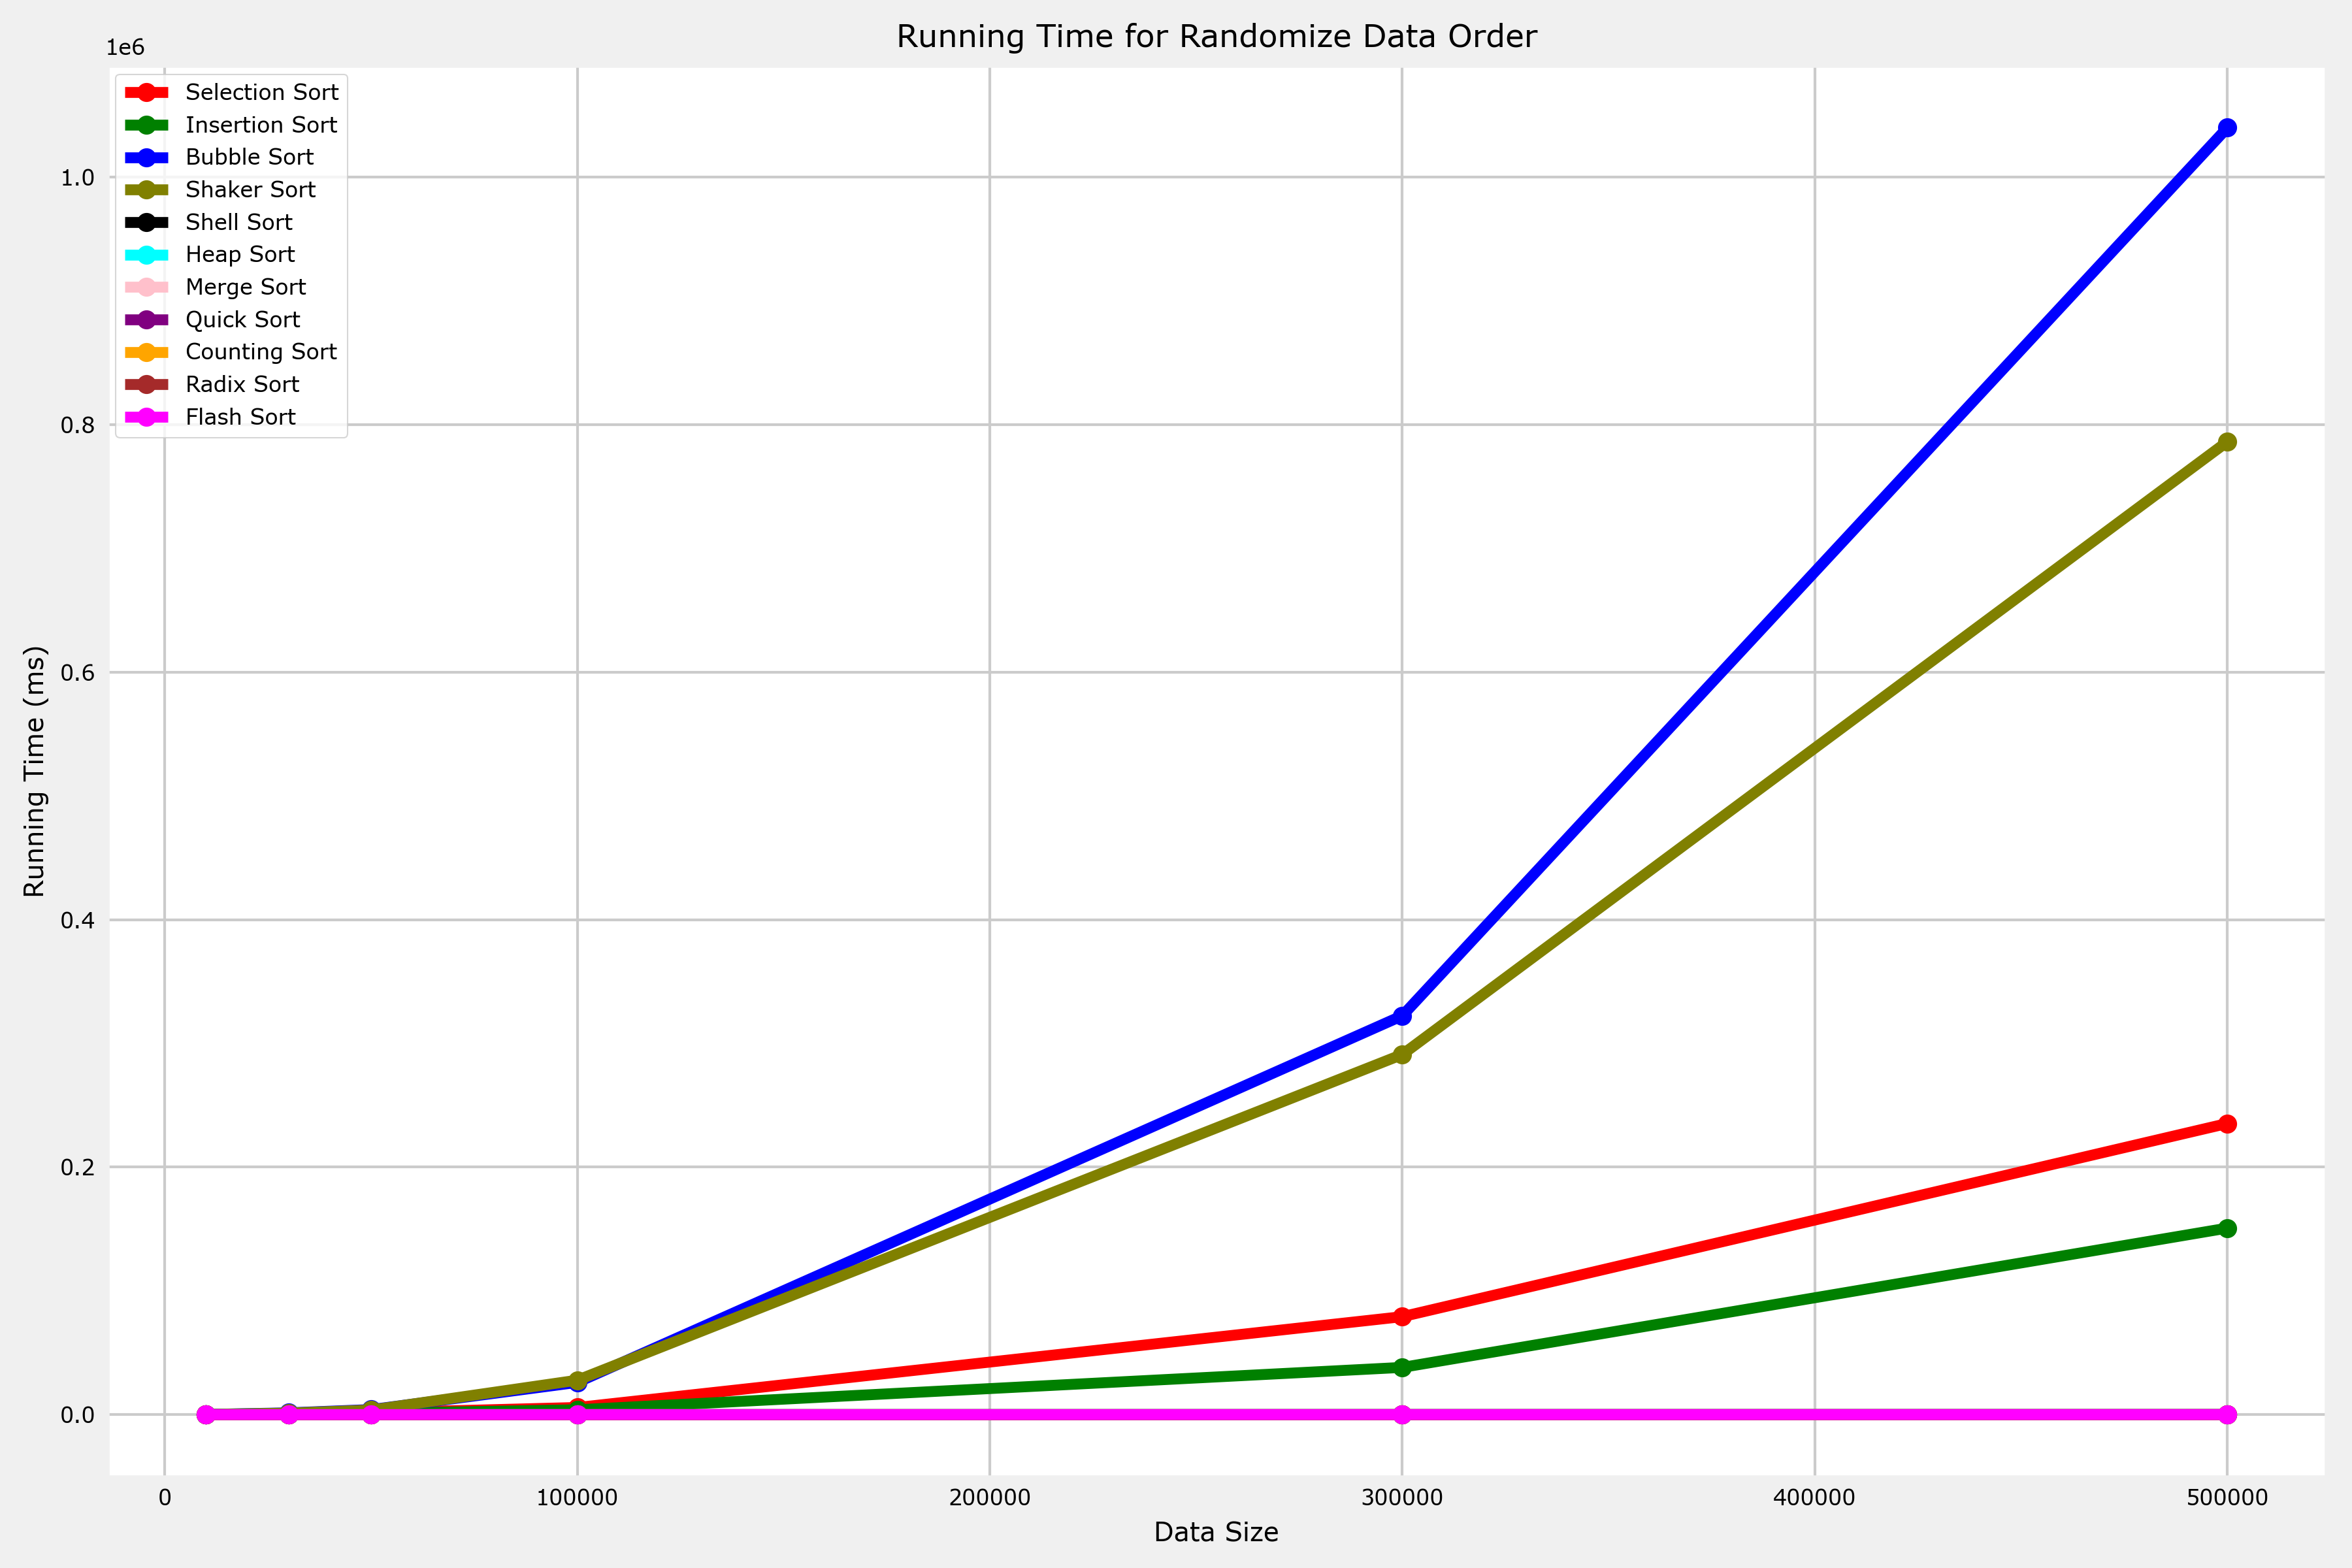
\includegraphics[width=0.8\textwidth]{img/results/randomize_running_time.png}
    \caption{Thời gian chạy của 11 thuật toán với dữ liệu ngẫu nhiên}
\end{figure}



\begin{figure}[H]
    \centering
    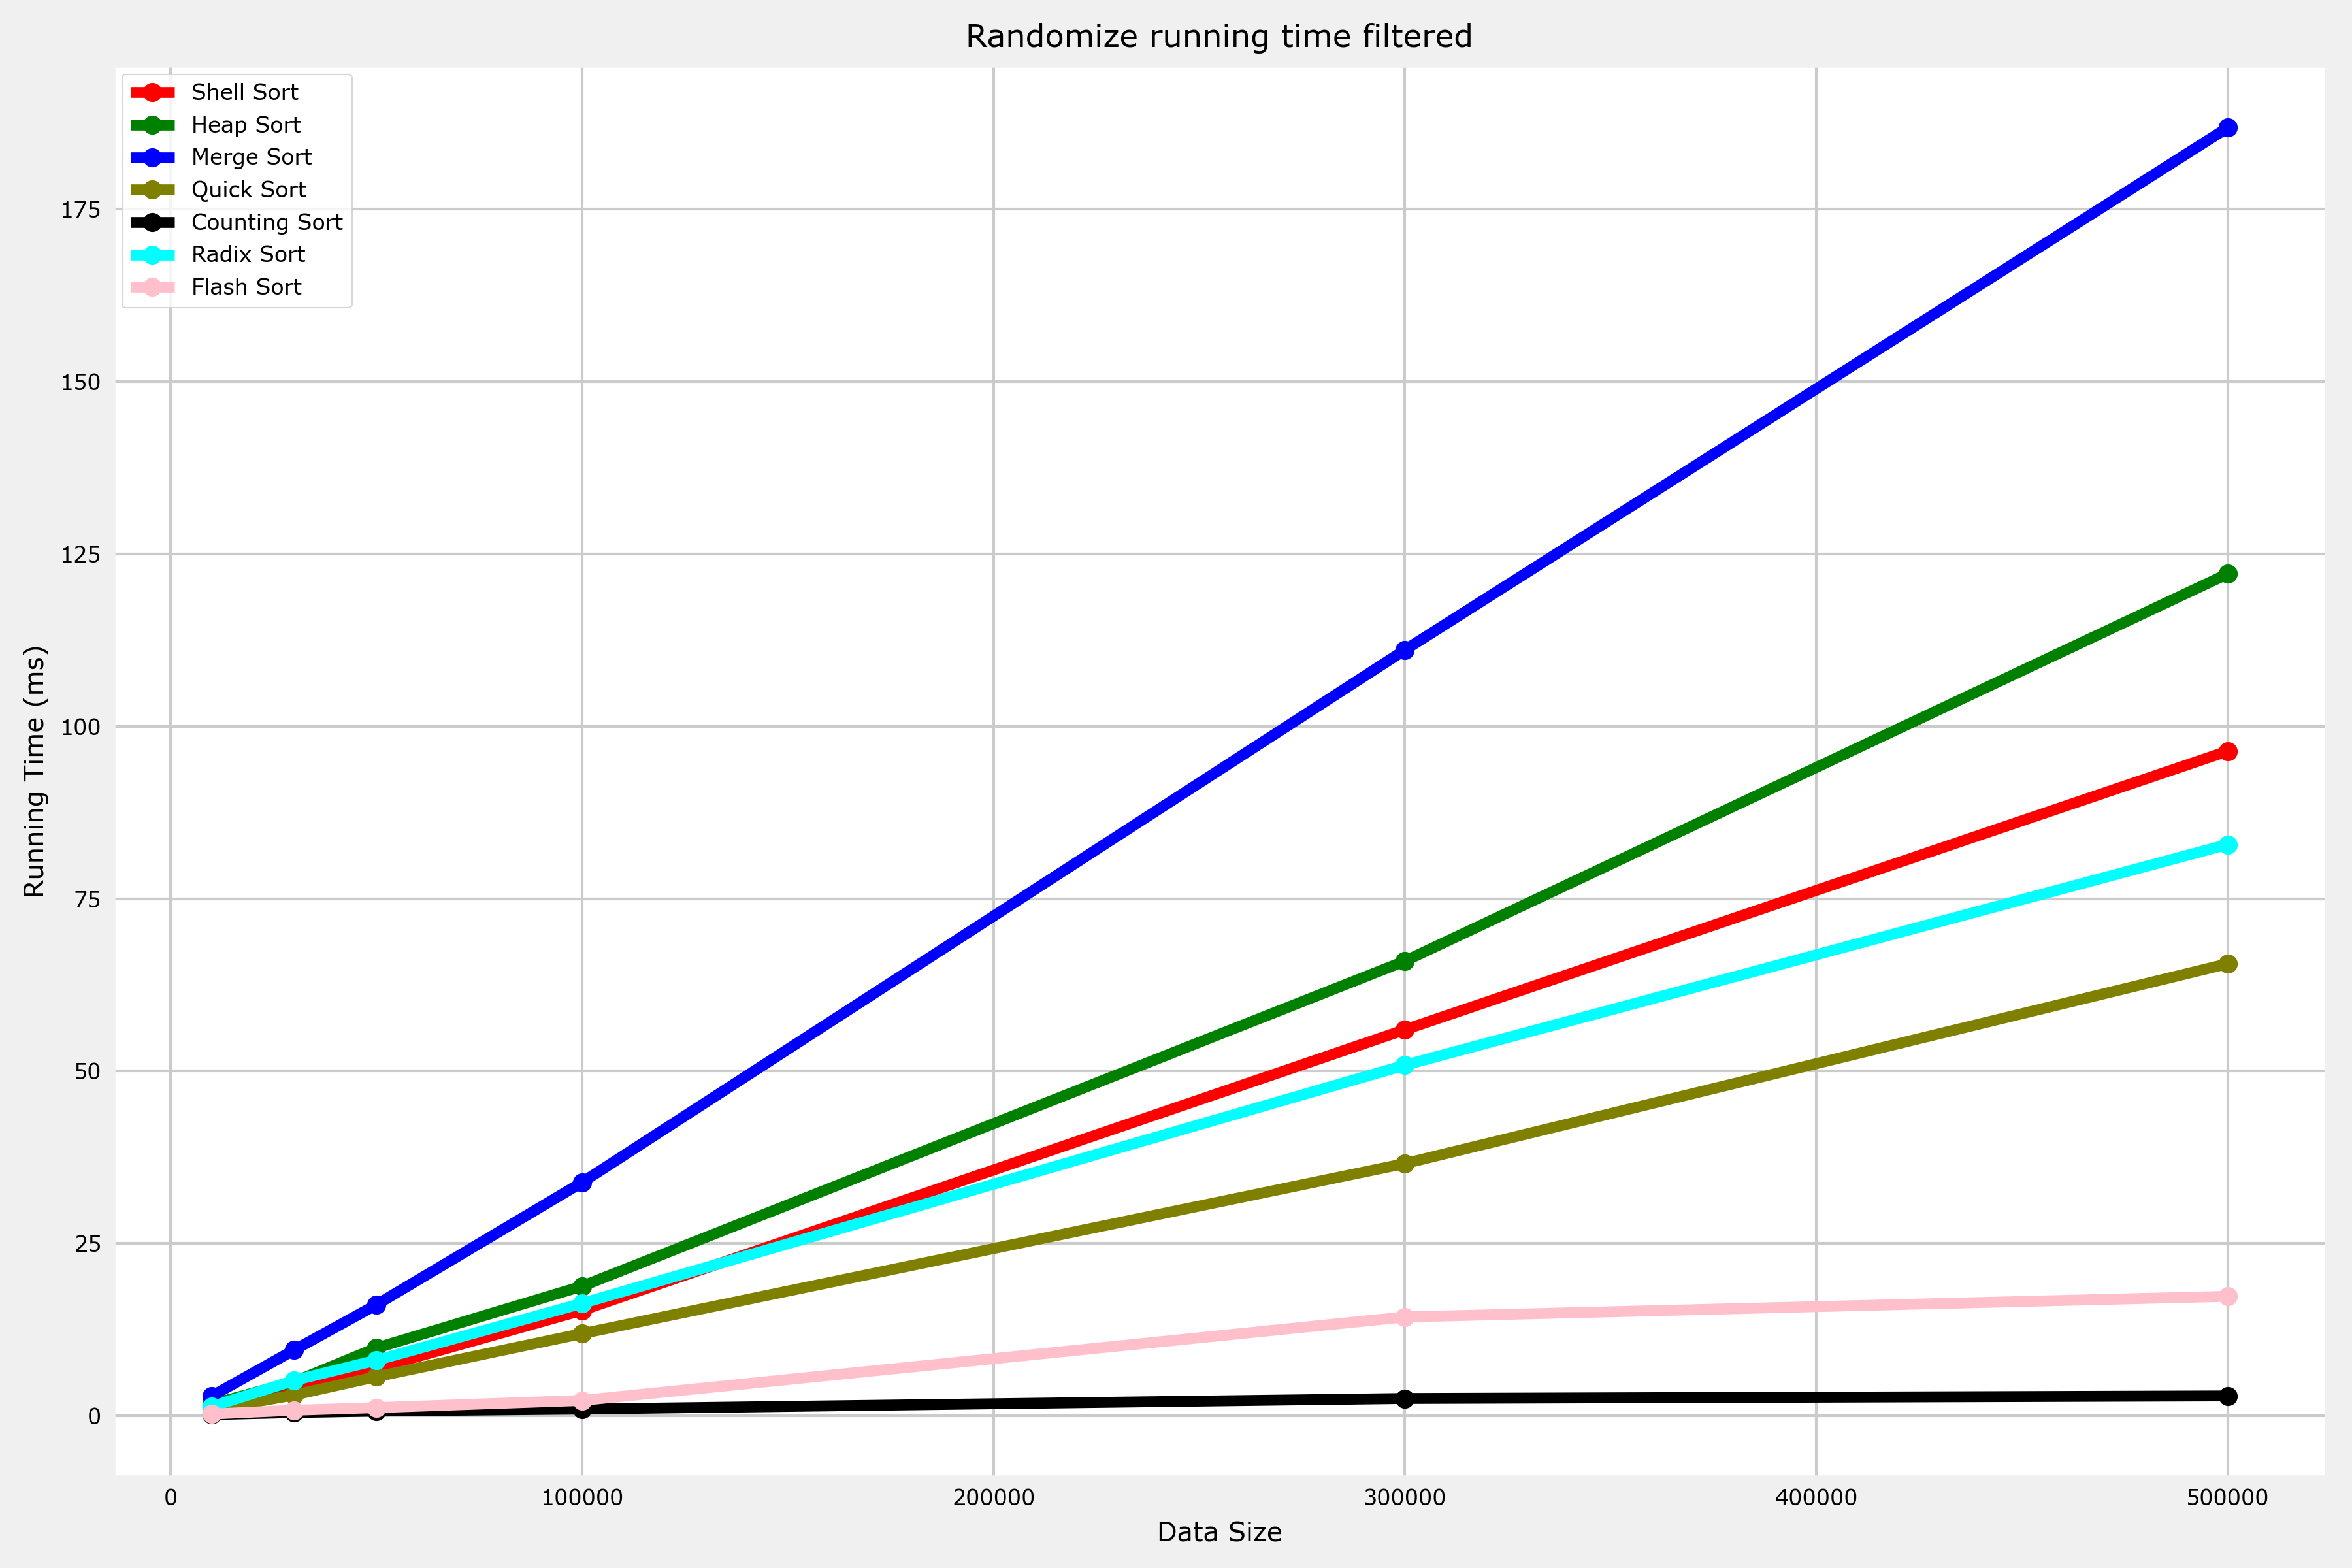
\includegraphics[width=0.8\textwidth]{img/results/randomize_running_time_filtered.png}
    \caption{Thời gian chạy của 11 thuật toán với dữ liệu ngẫu nhiên sau khi loại bỏ outlier}
\end{figure}



\paragraph{2. Dữ liệu gần sắp xếp hoàn chỉnh}
\begin{figure}[H]
    \centering
    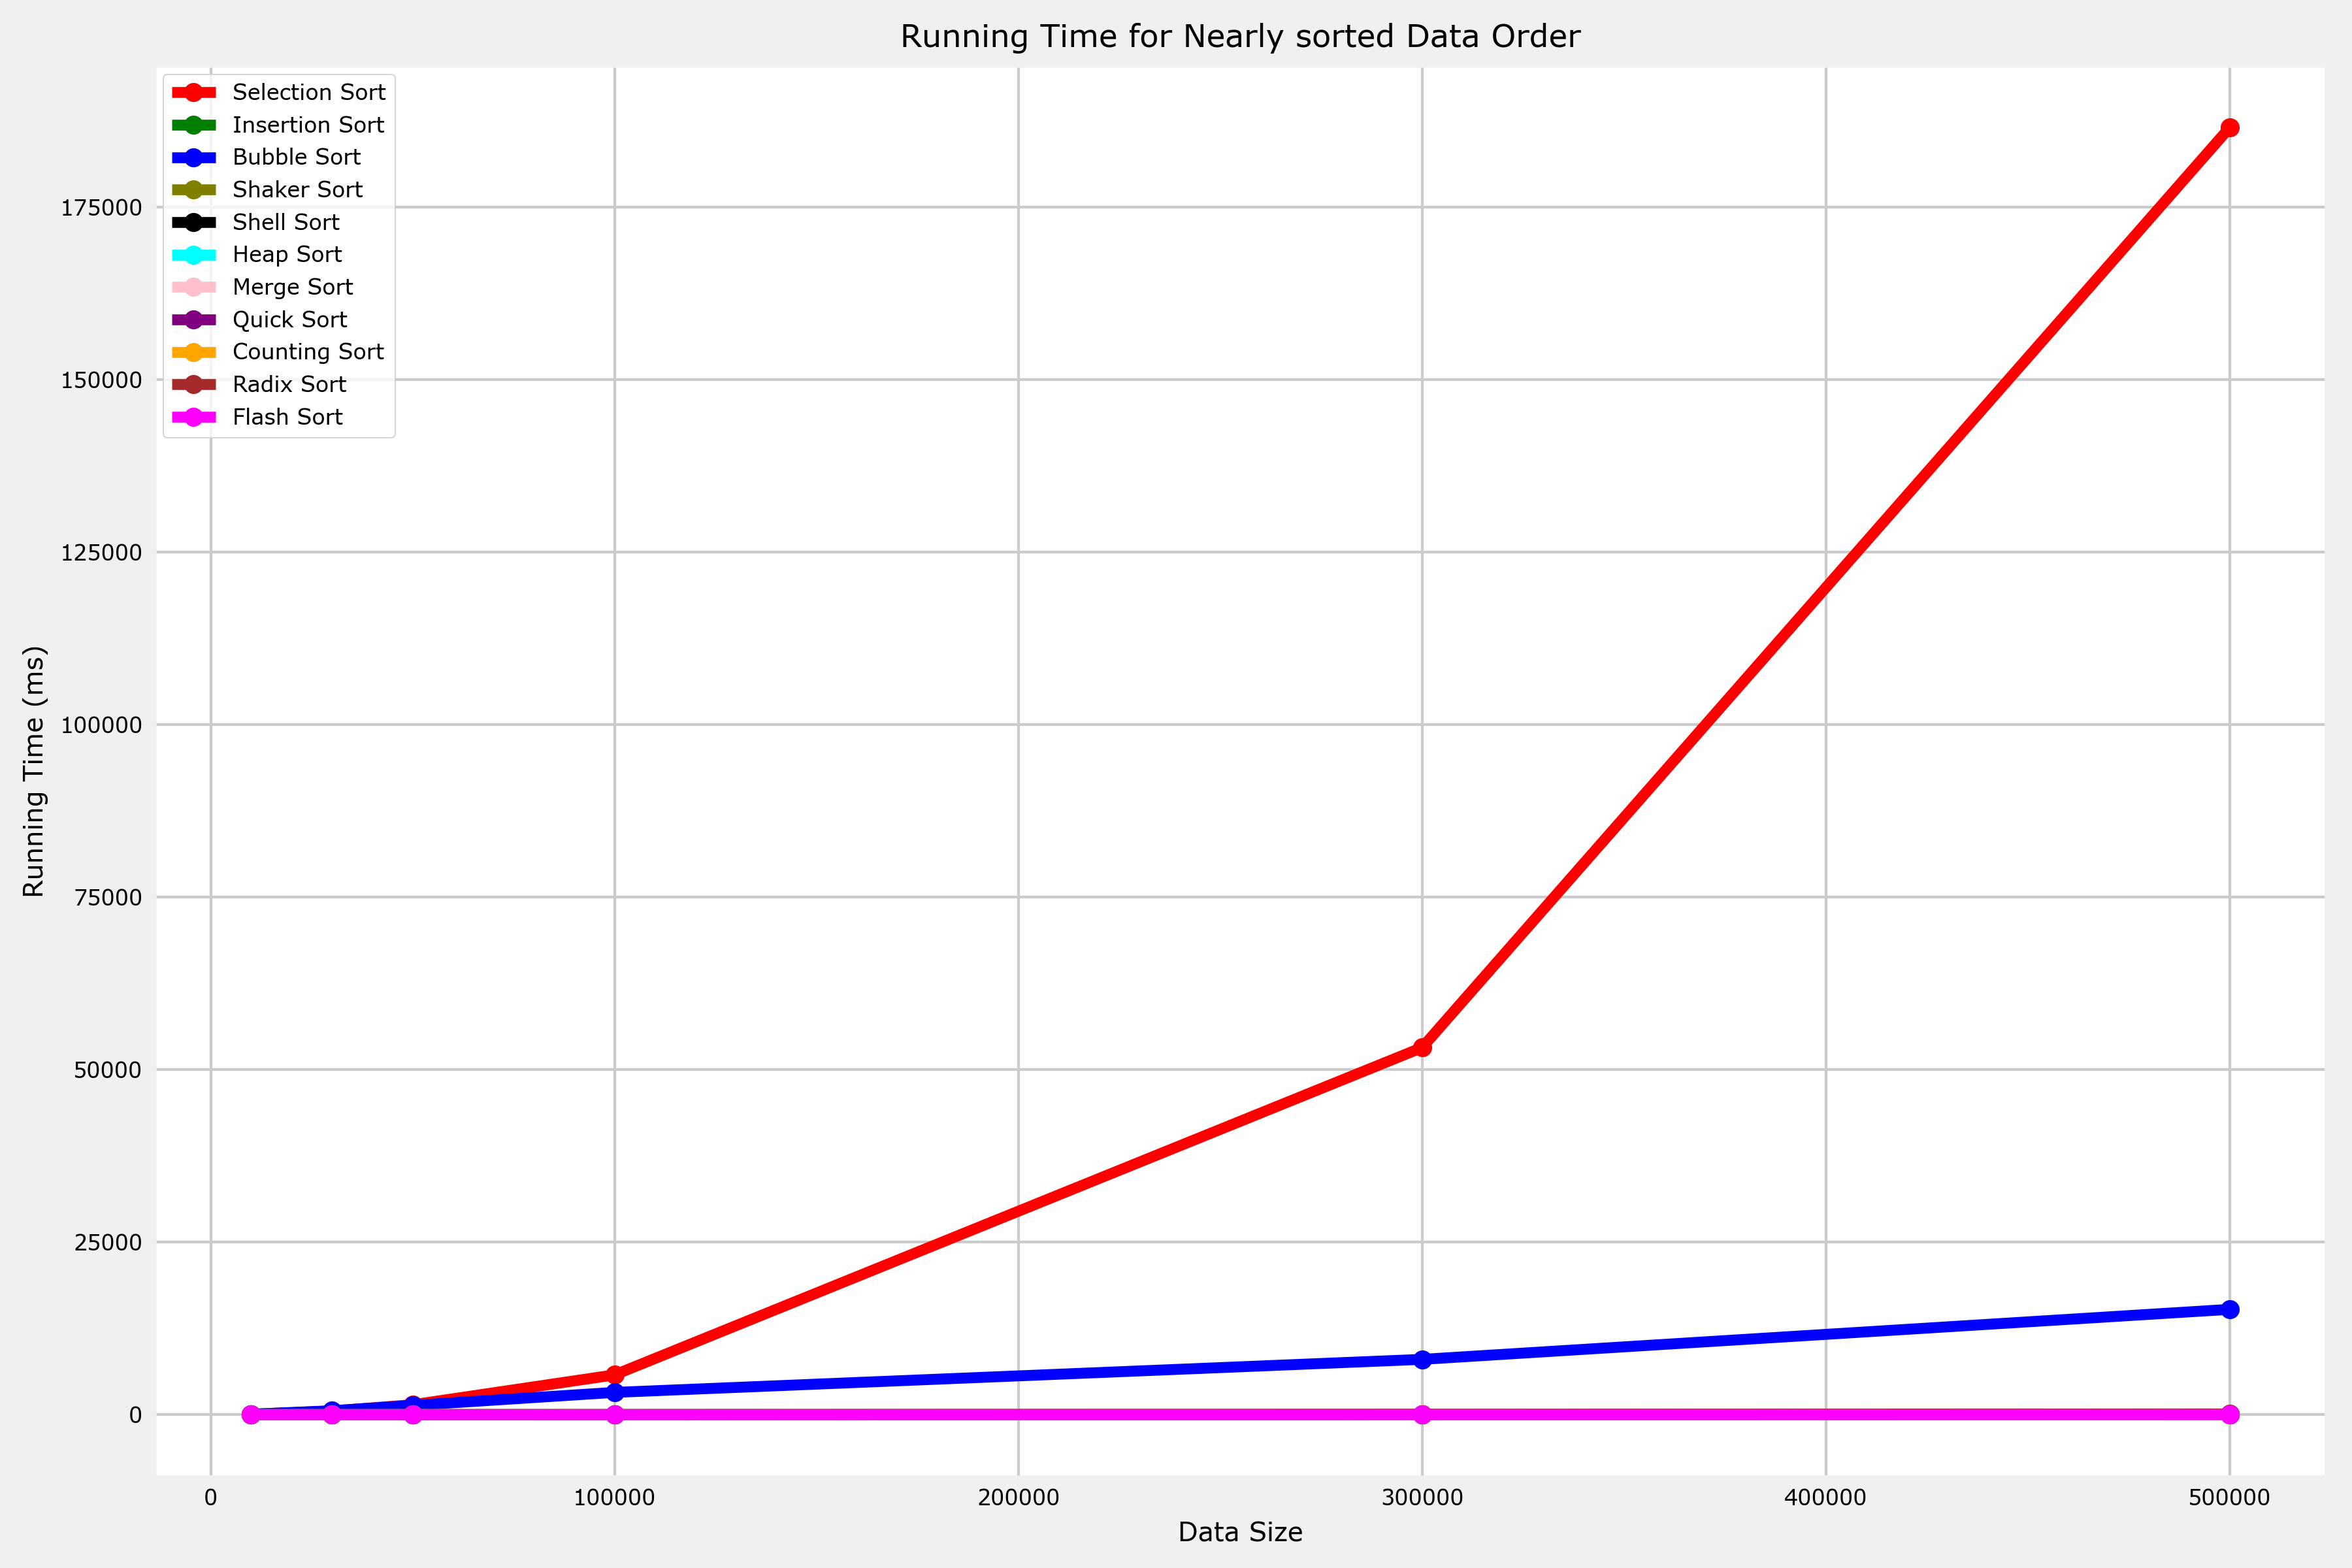
\includegraphics[width=0.8\textwidth]{img/results/nearly_sorted_running_time.png}
    \caption{Thời gian chạy của 11 thuật toán với dữ liệu gần sắp xếp hoàn chỉnh}
\end{figure}

\begin{figure}[H]
    \centering
    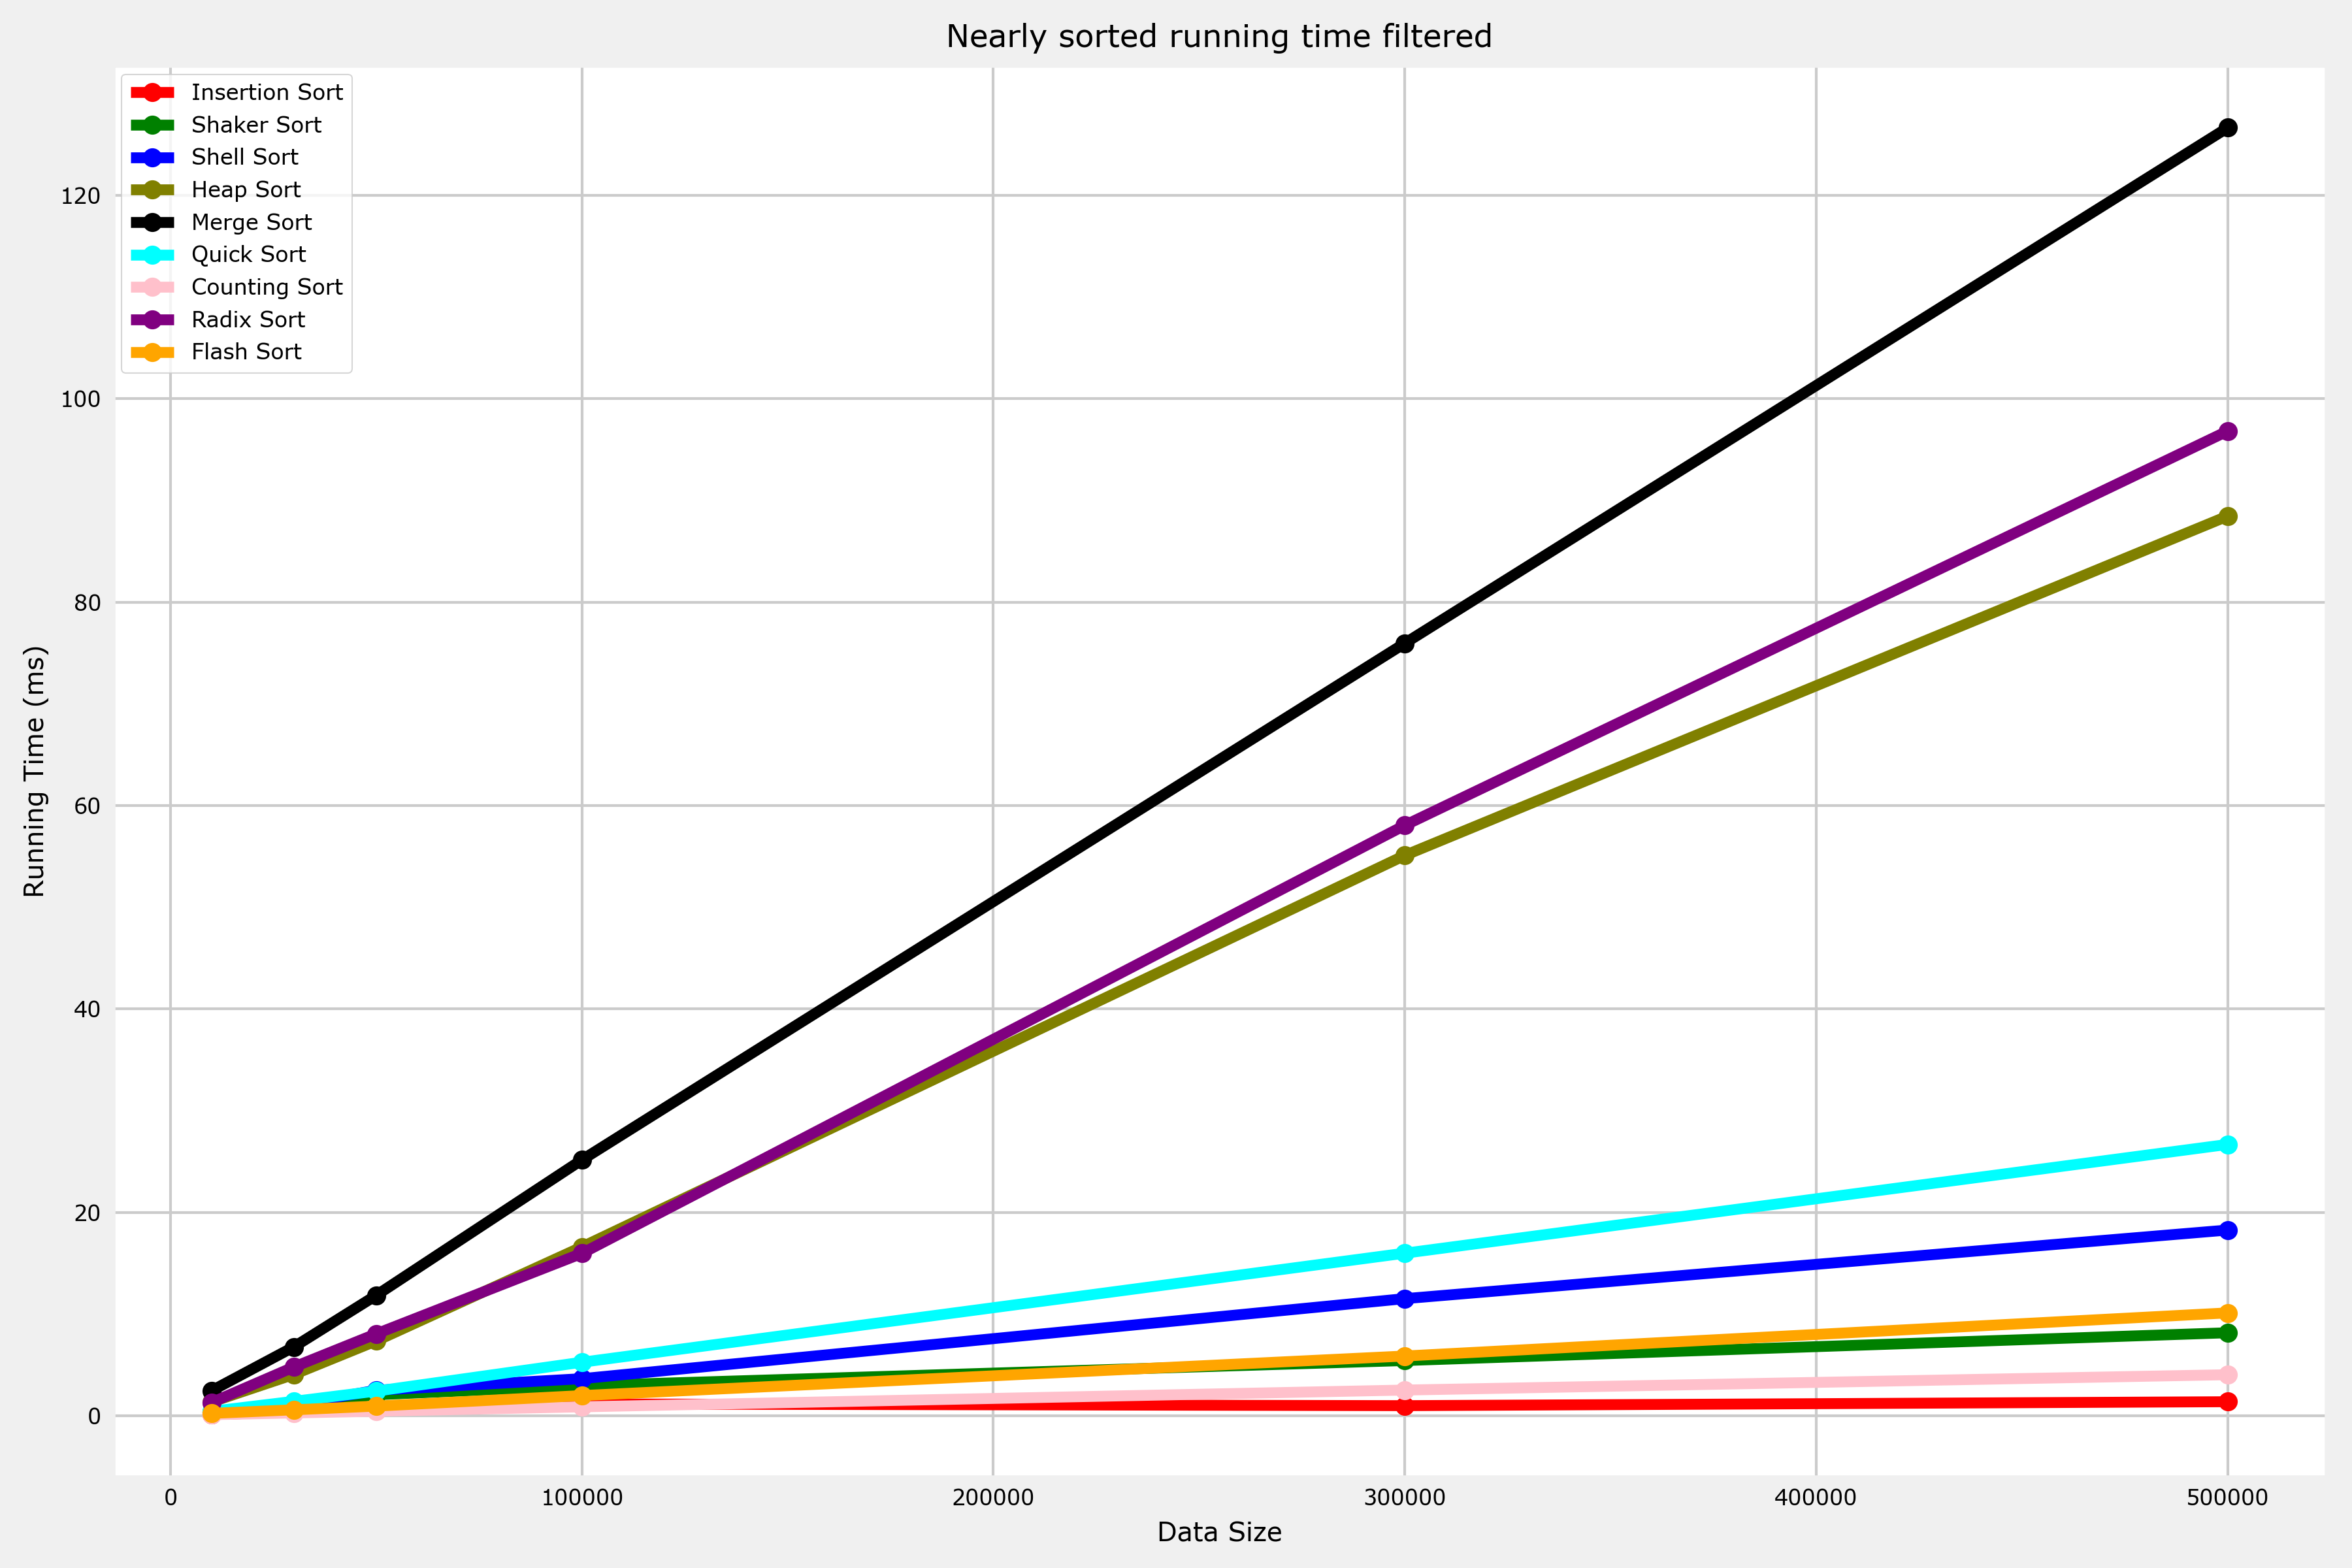
\includegraphics[width=0.8\textwidth]{img/results/nearly_sorted_running_time_filtered.png}
    \caption{Thời gian chạy của 11 thuật toán với dữ liệu gần sắp xếp hoàn chỉnh sau khi loại bỏ outlier}
\end{figure}


\paragraph{3. Dữ liệu được sắp xếp}
\begin{figure}[H]
    \centering
    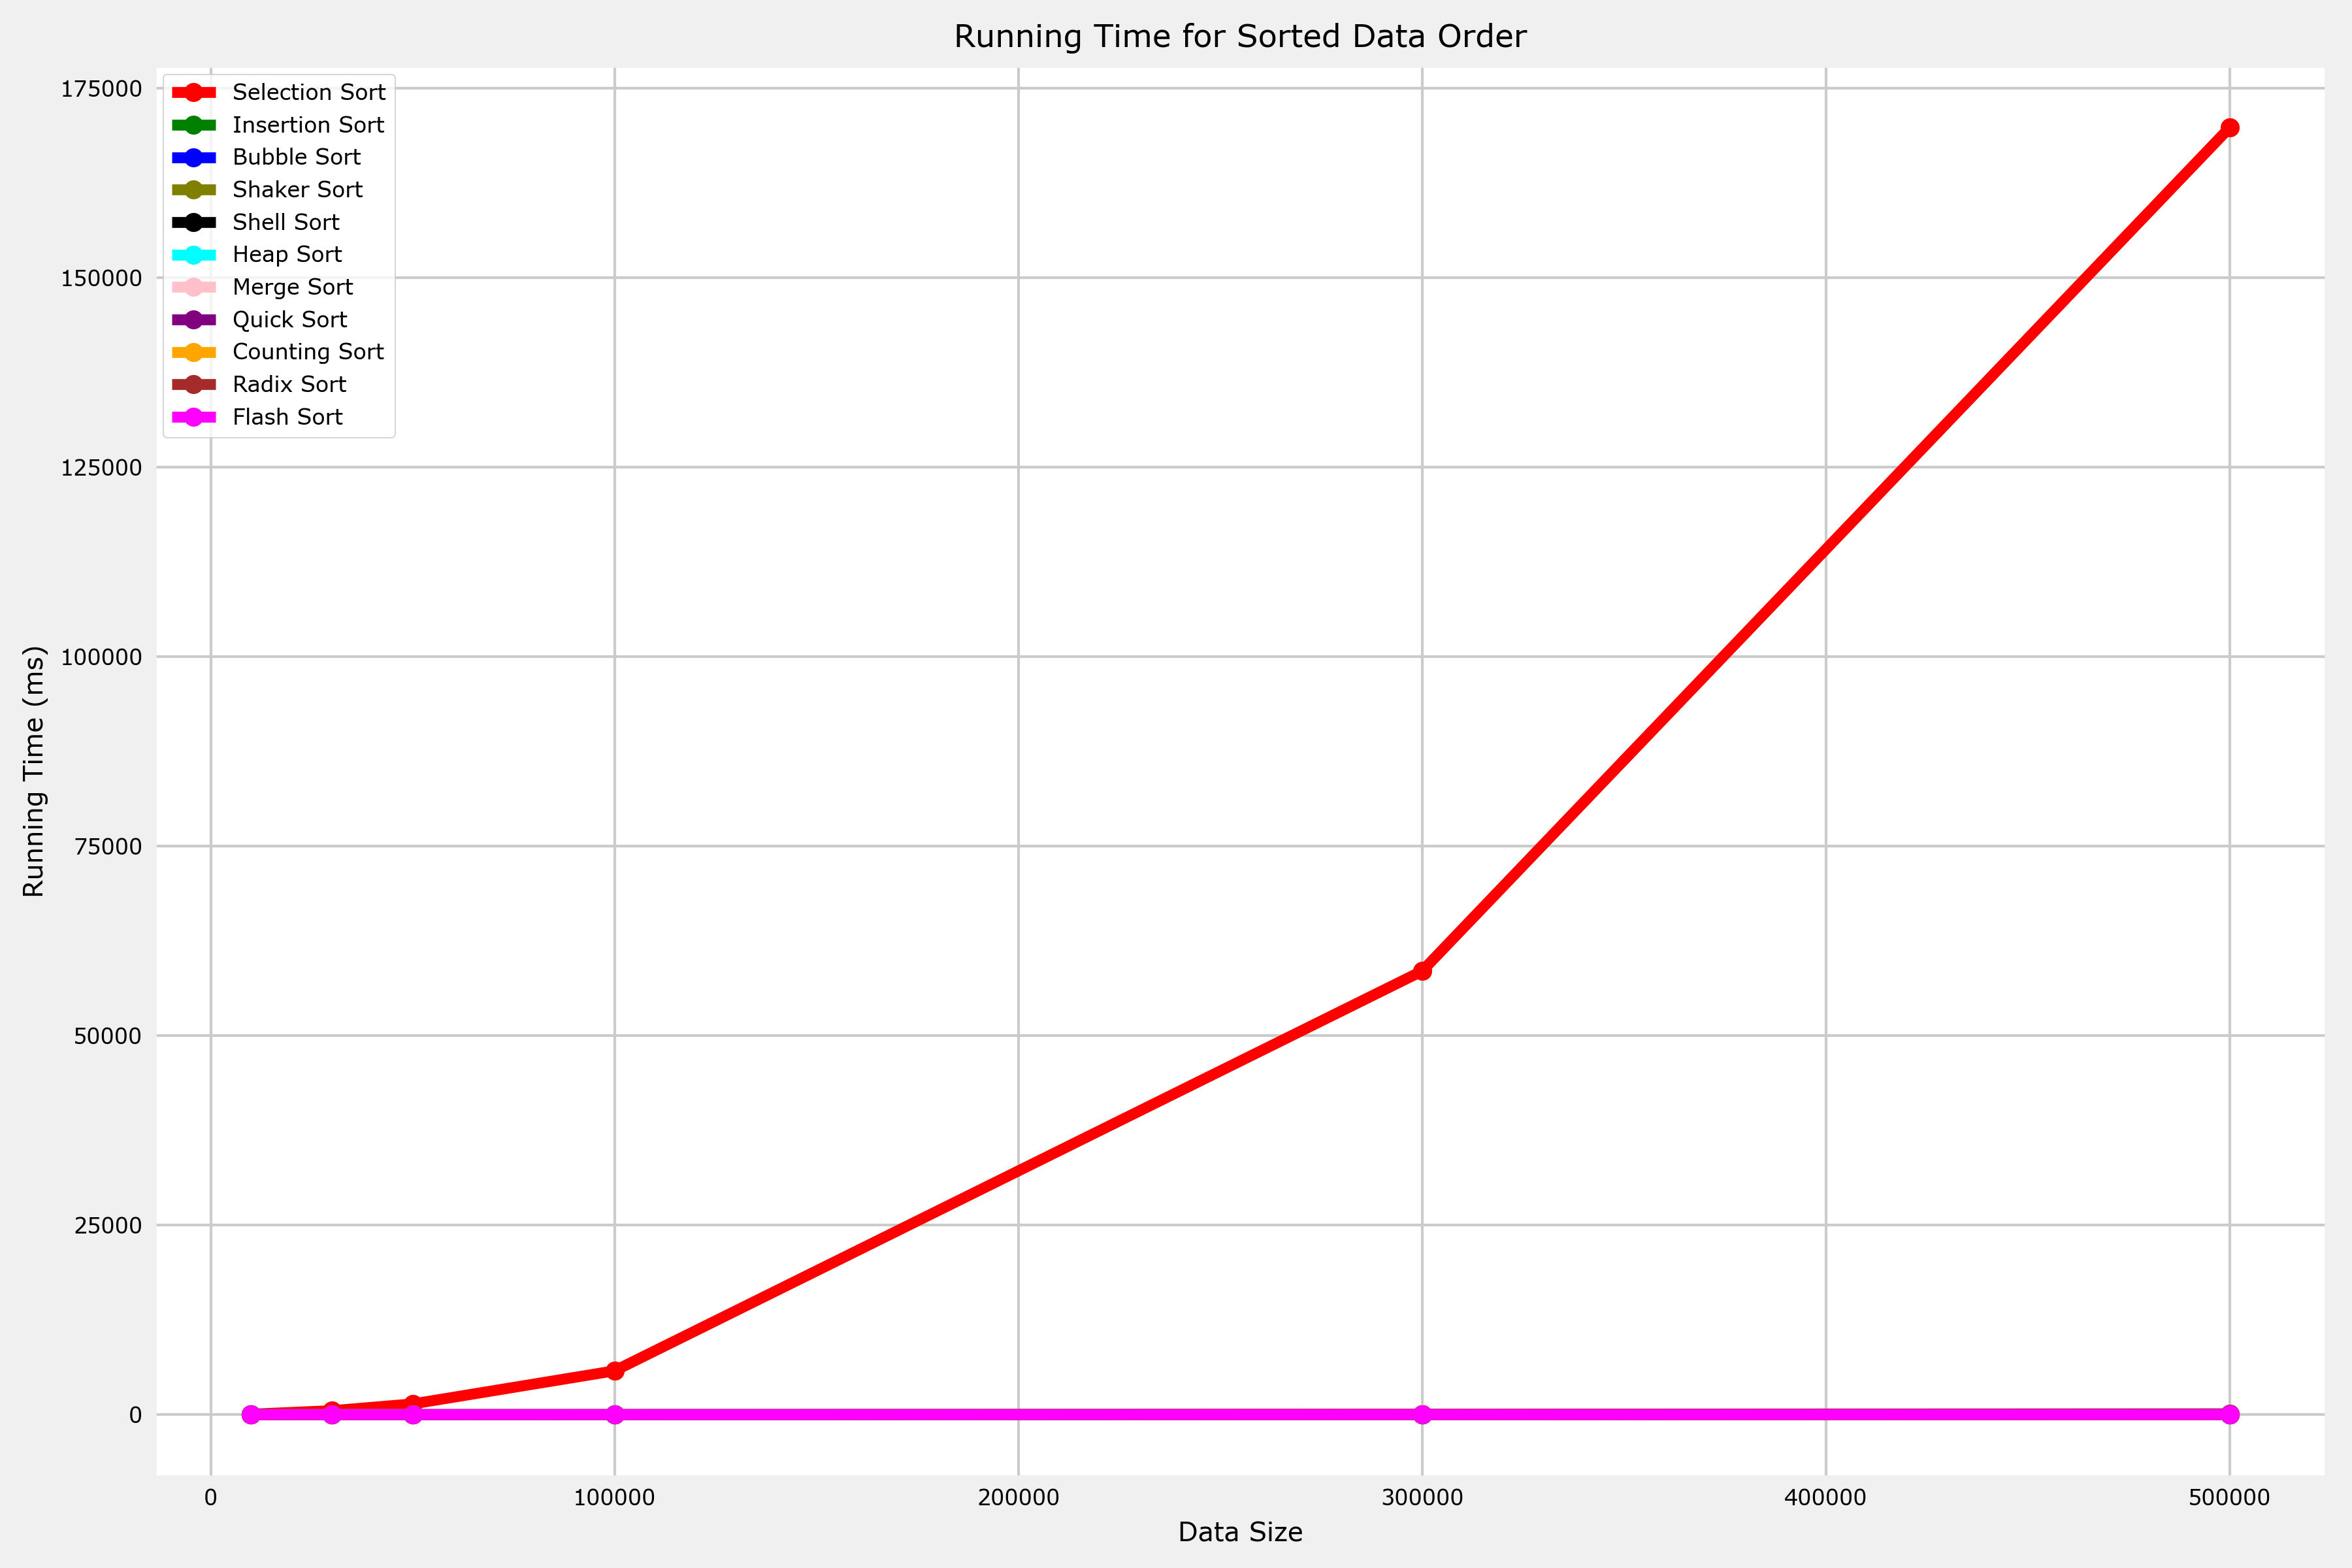
\includegraphics[width=0.8\textwidth]{img/results/sorted_running_time.png}
    \caption{Thời gian chạy của 11 thuật toán với dữ liệu được sắp xếp}
\end{figure}

\begin{figure}[H]
    \centering
    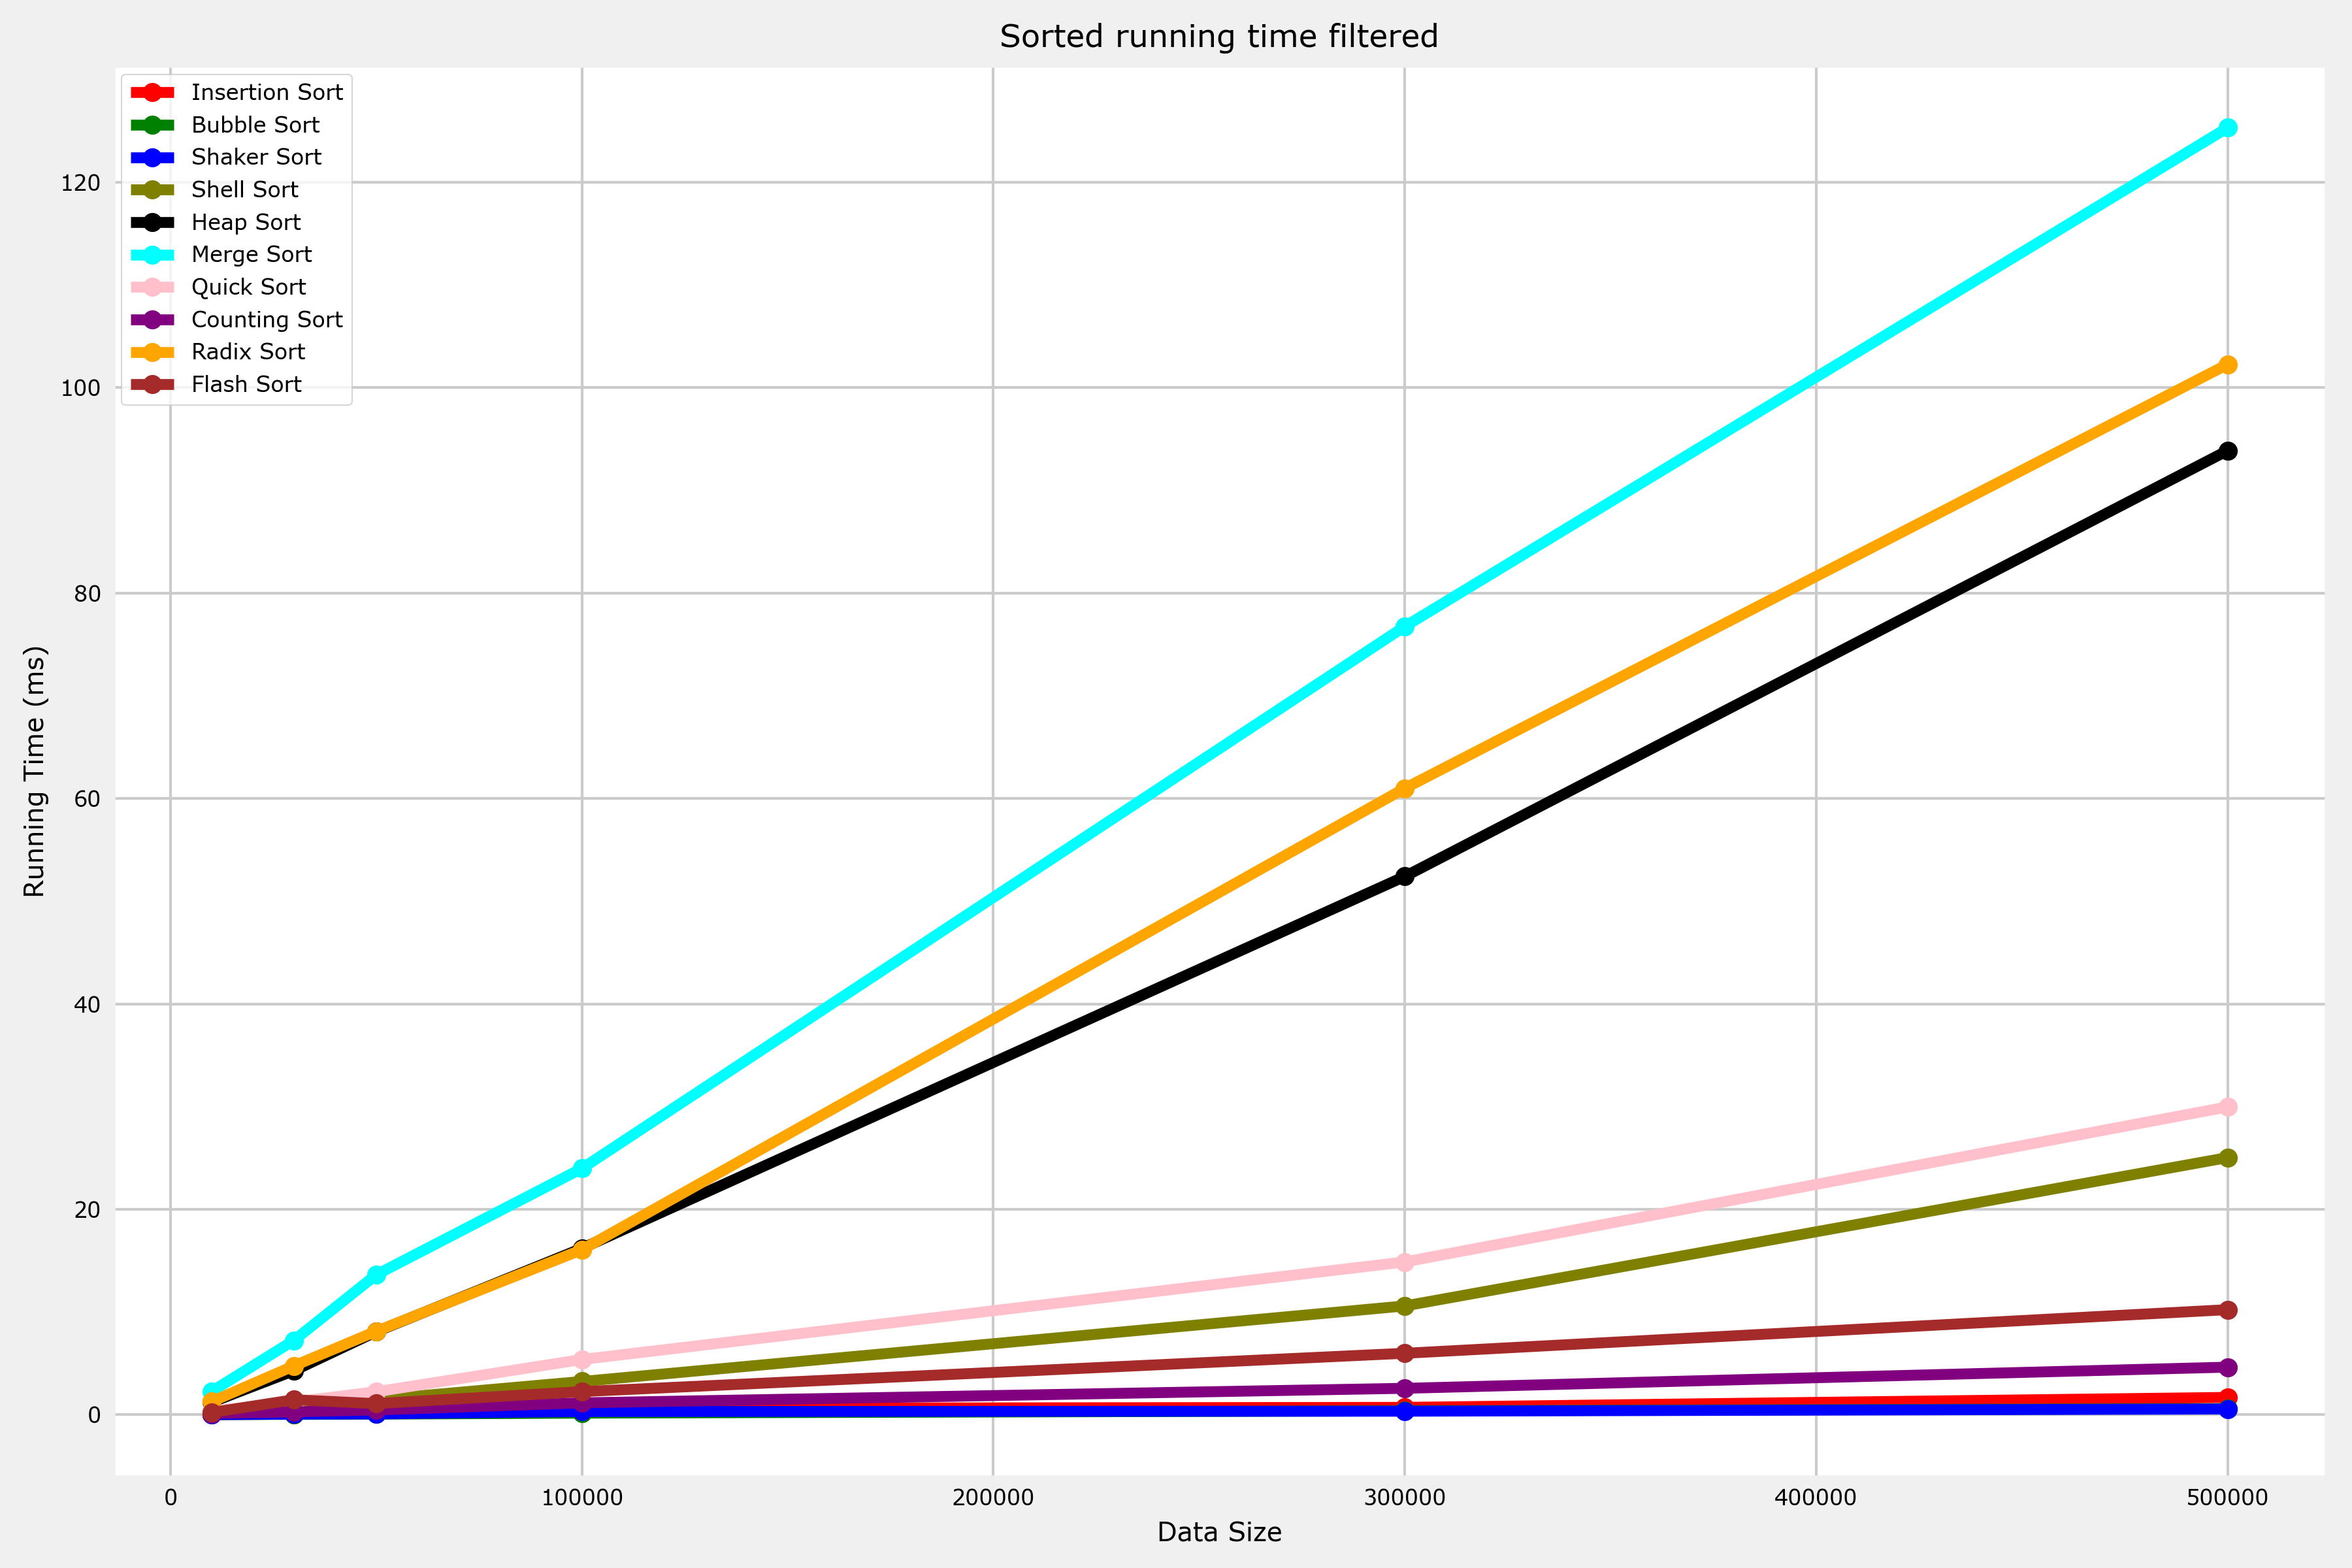
\includegraphics[width=0.8\textwidth]{img/results/sorted_running_time_filtered.png}
    \caption{Thời gian chạy của 11 thuật toán với dữ liệu được sắp xếp sau khi loại bỏ outlier}
\end{figure}




\paragraph{4. Dữ liệu đảo ngược}
\begin{figure}[H]
    \centering
    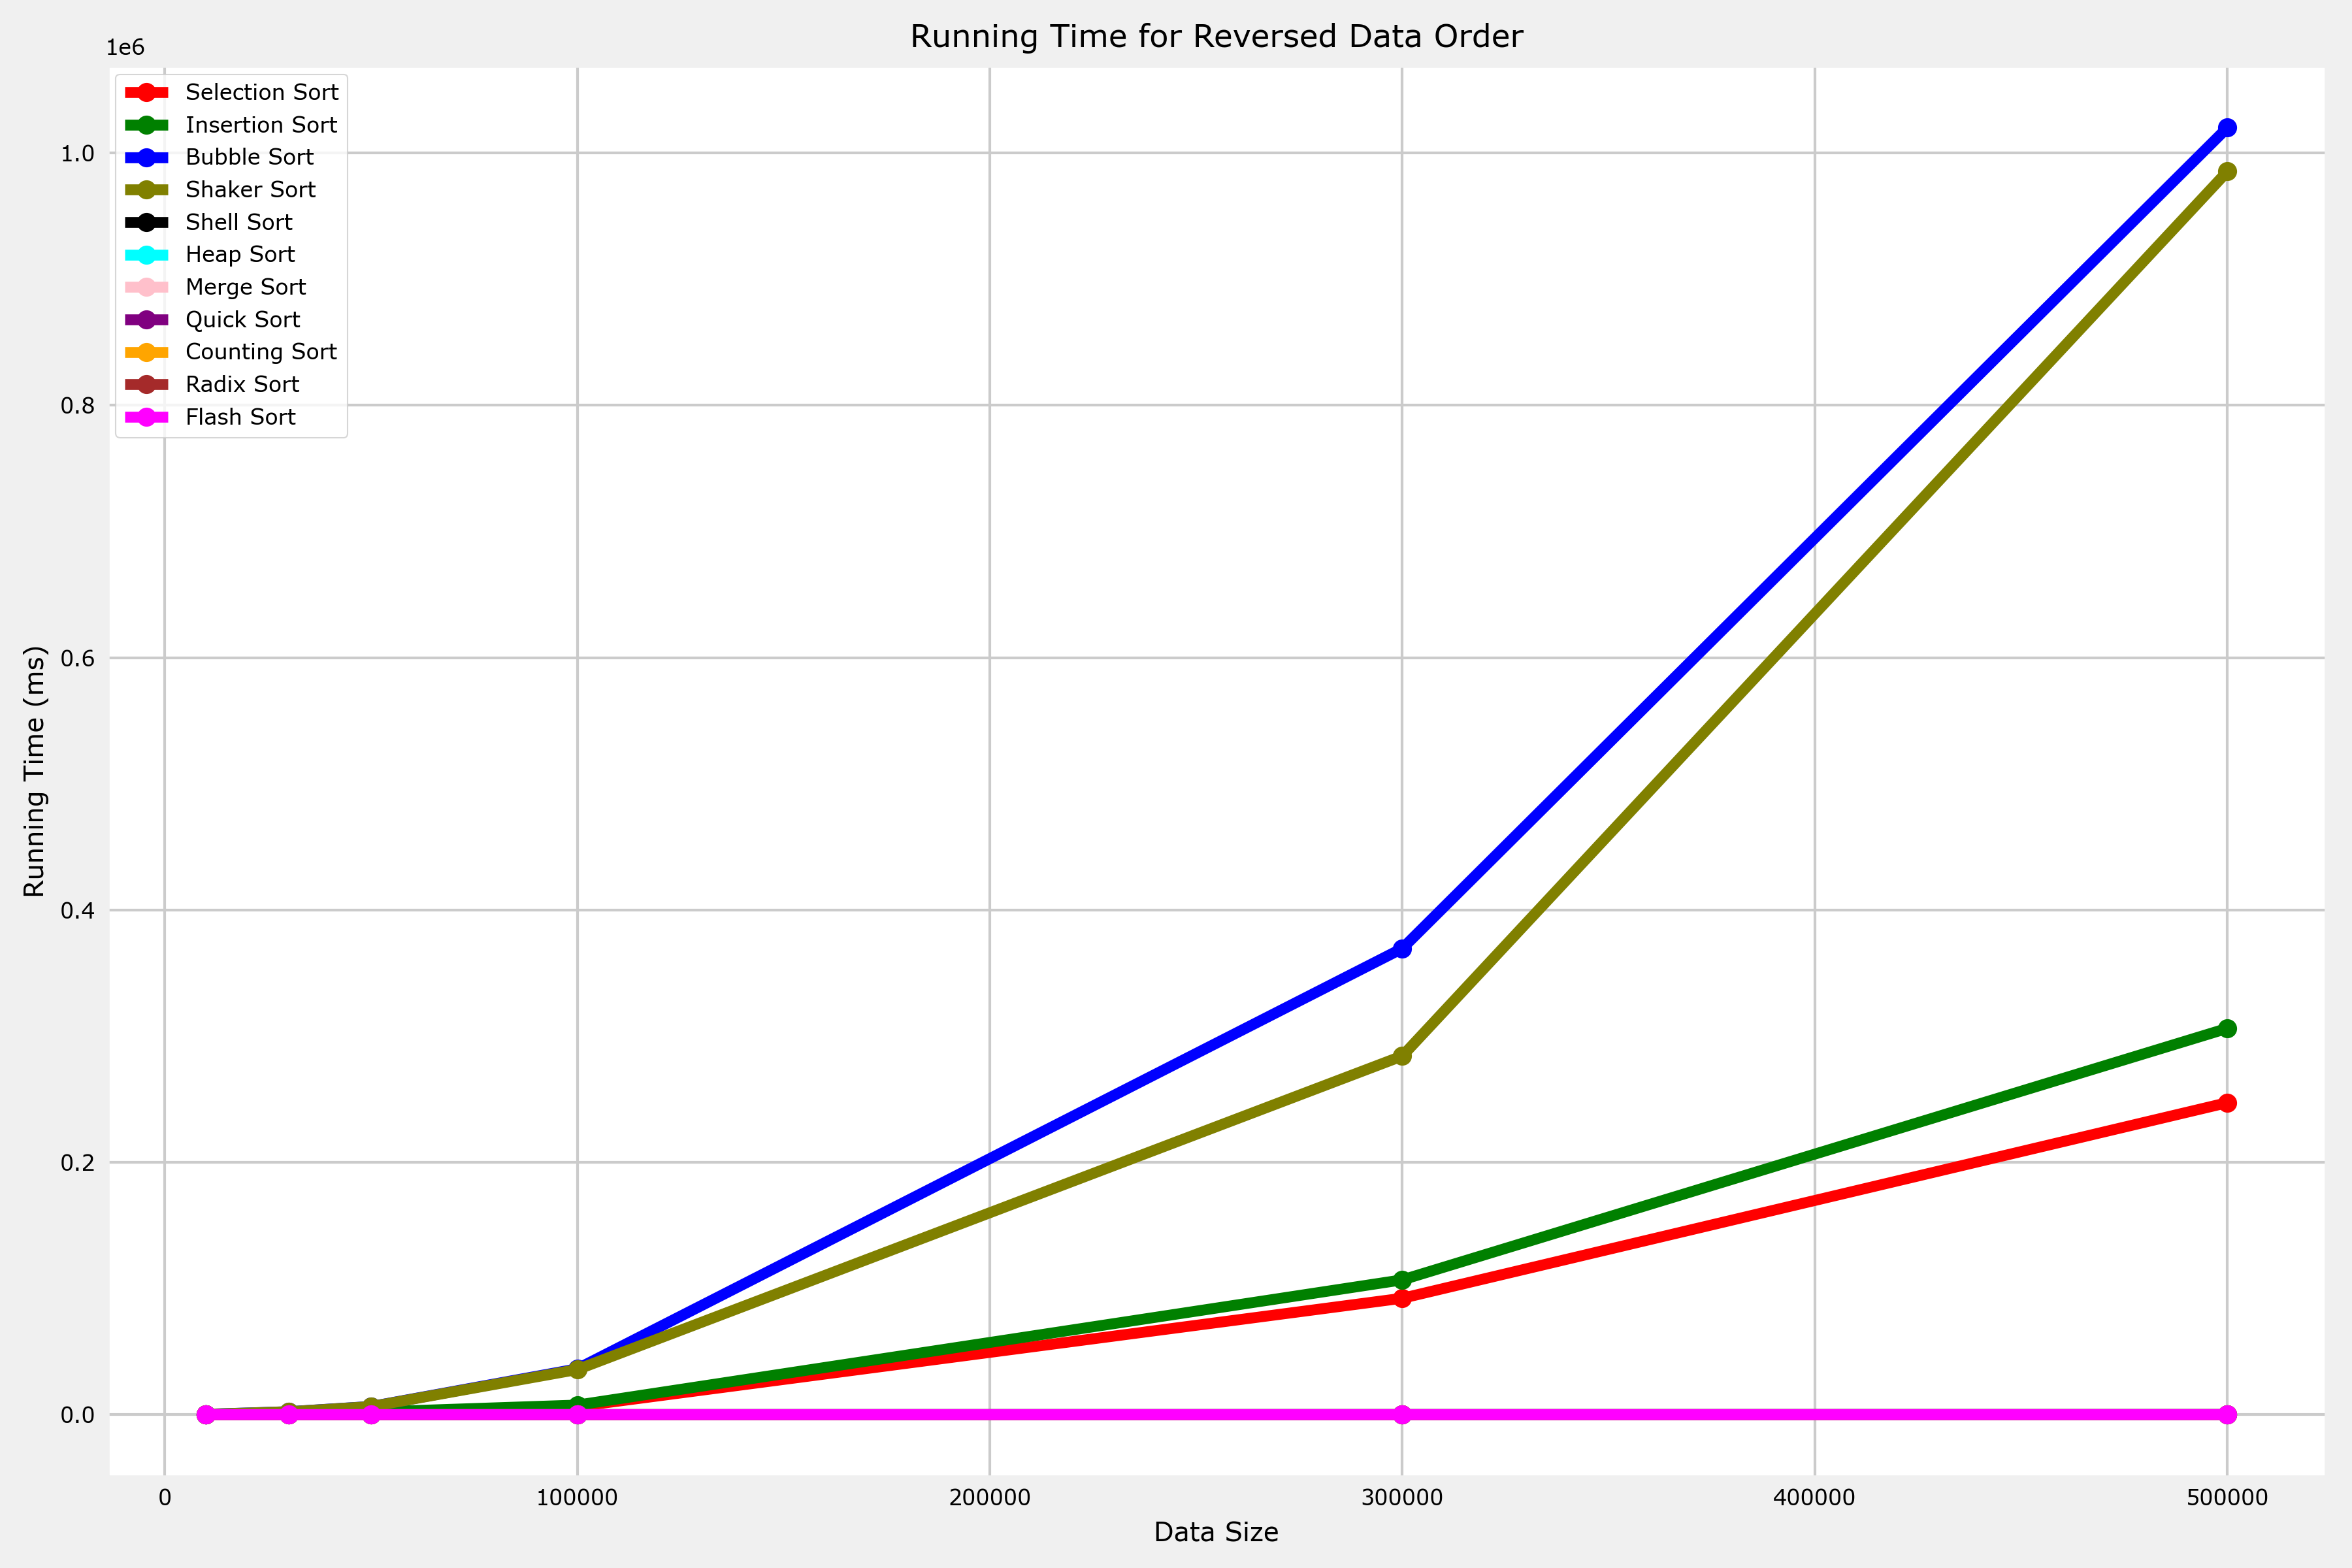
\includegraphics[width=0.8\textwidth]{img/results/reversed_running_time.png}
    \caption{Thời gian chạy của 11 thuật toán với dữ liệu đảo ngược}
\end{figure}

\begin{figure}[H]
    \centering
    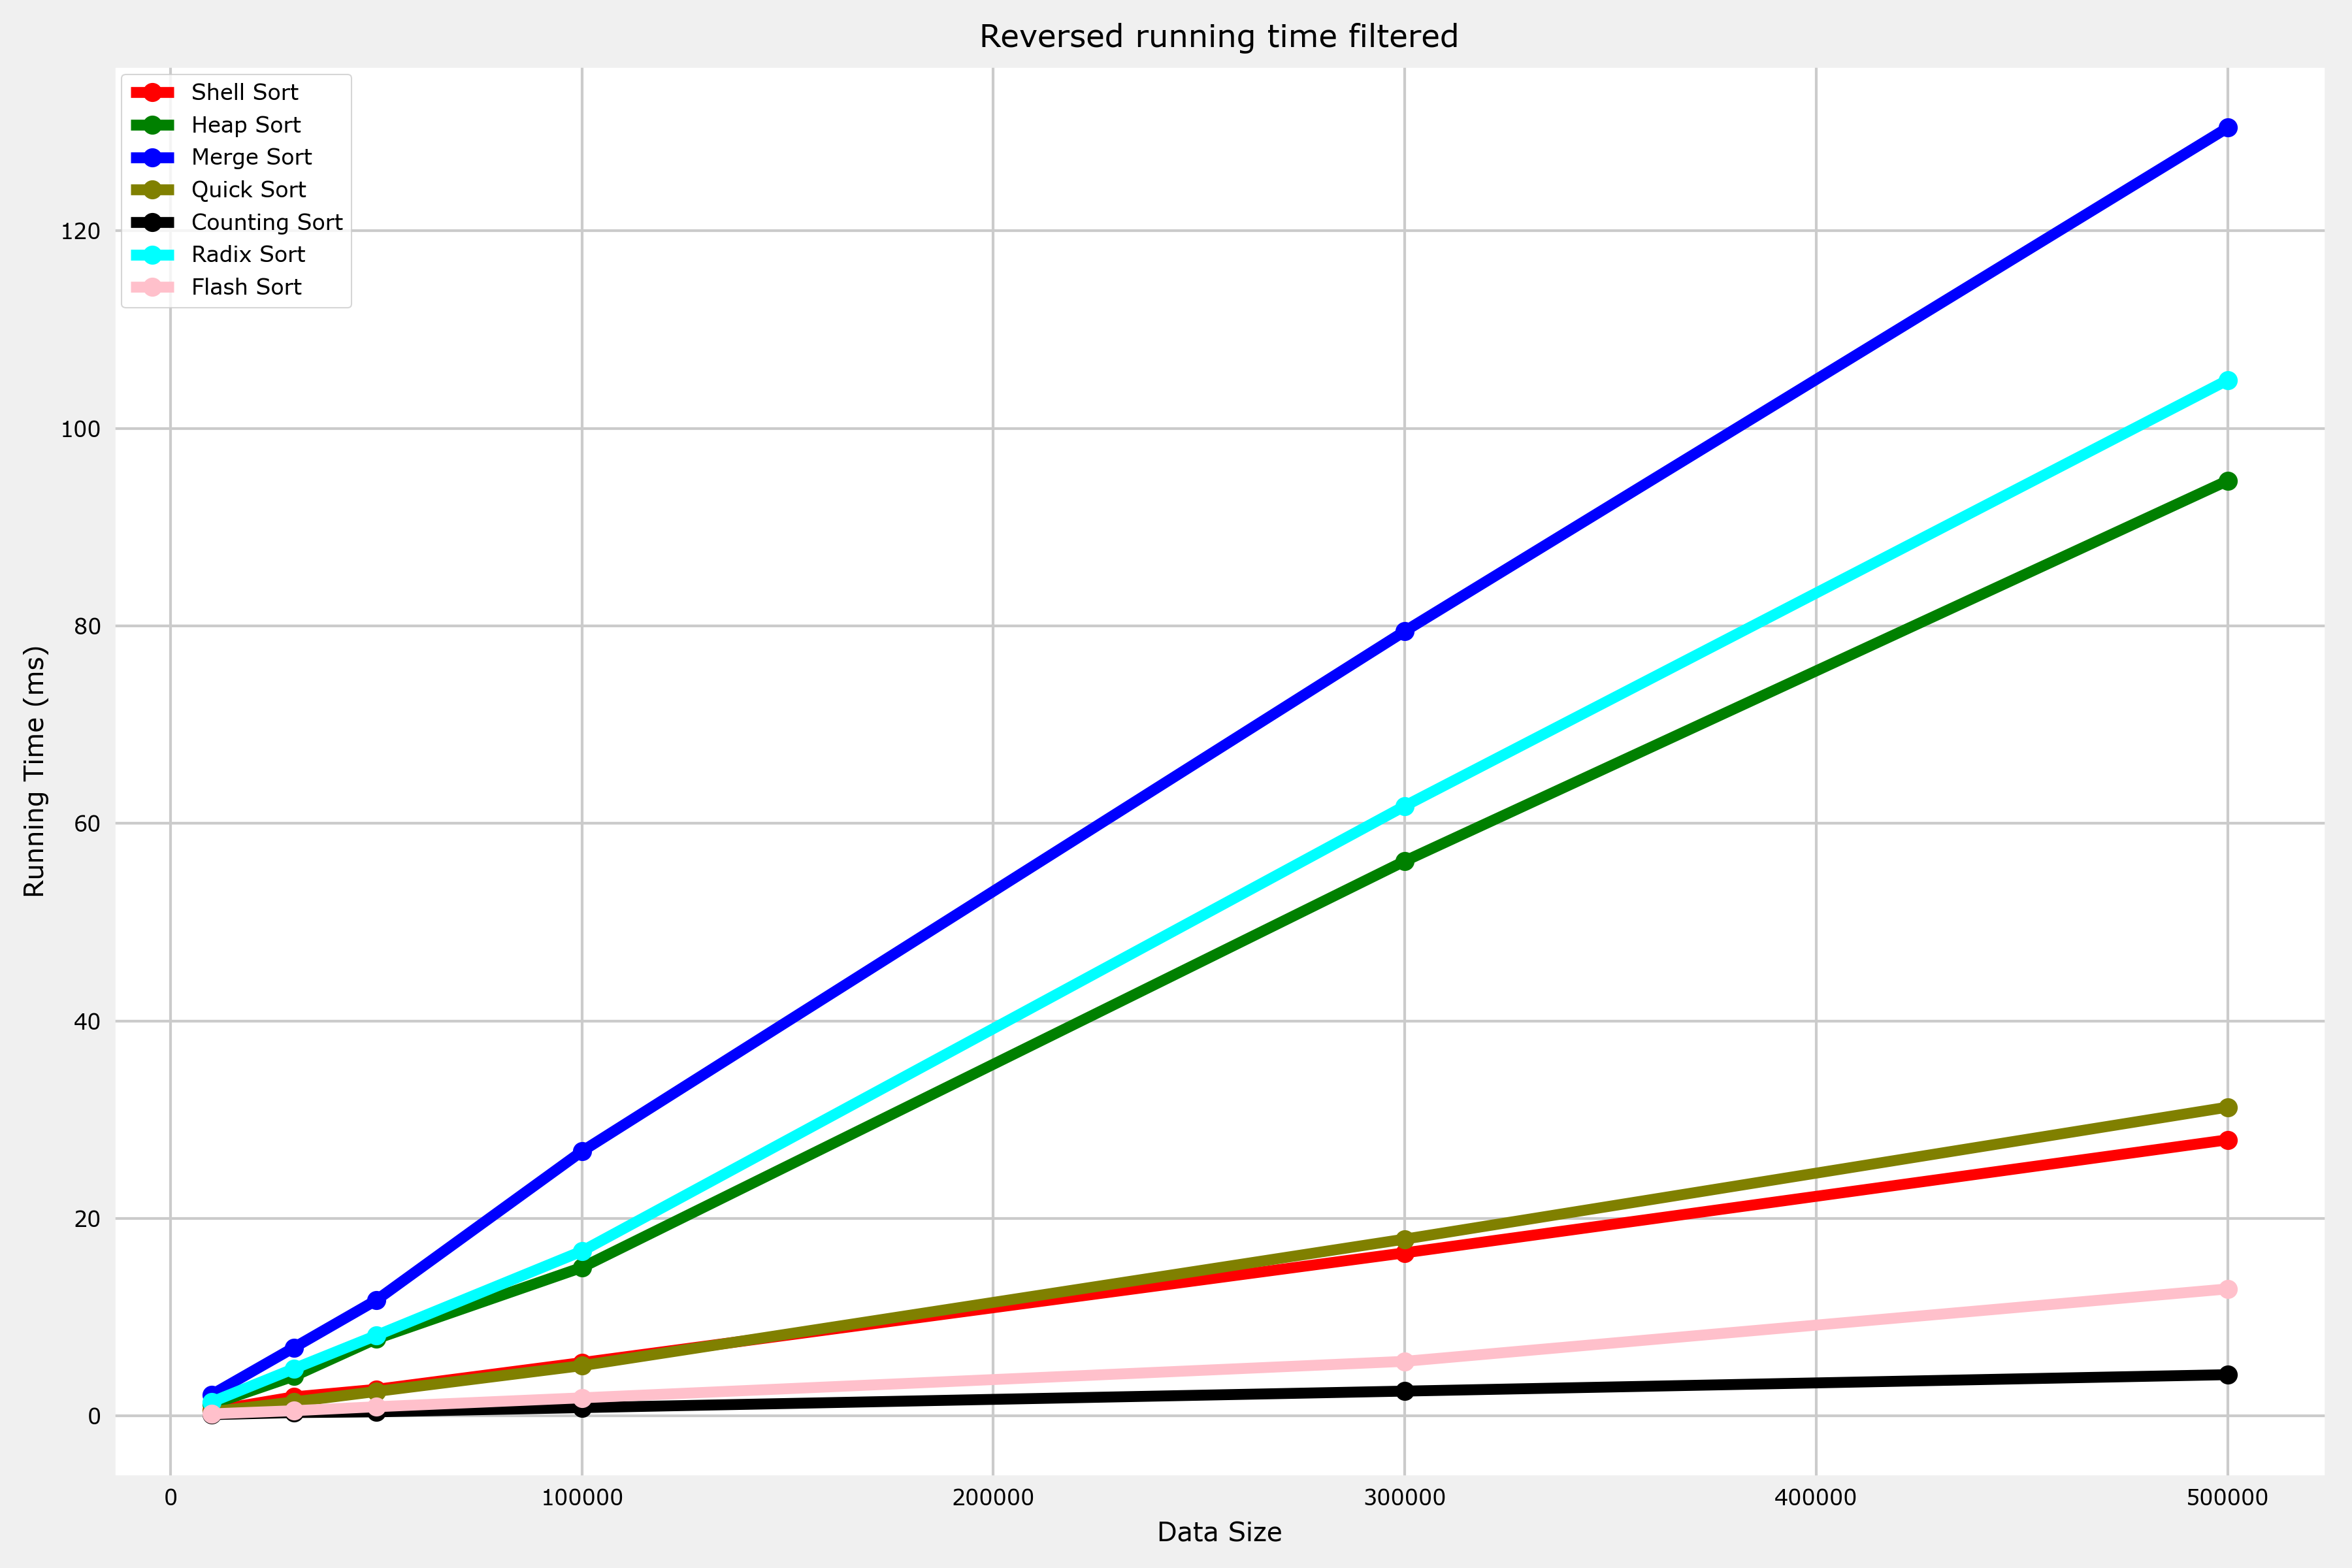
\includegraphics[width=0.8\textwidth]{img/results/reversed_running_time_filtered.png}
    \caption{
        Thời gian chạy của 11 thuật toán với dữ liệu đảo ngược sau khi loại bỏ outlier
    }
\end{figure}











\subsubsection{Biểu đồ số phép so sánh}


\paragraph{1. Dữ liệu ngẫu nhiên}
\begin{figure}[H]
    \centering
    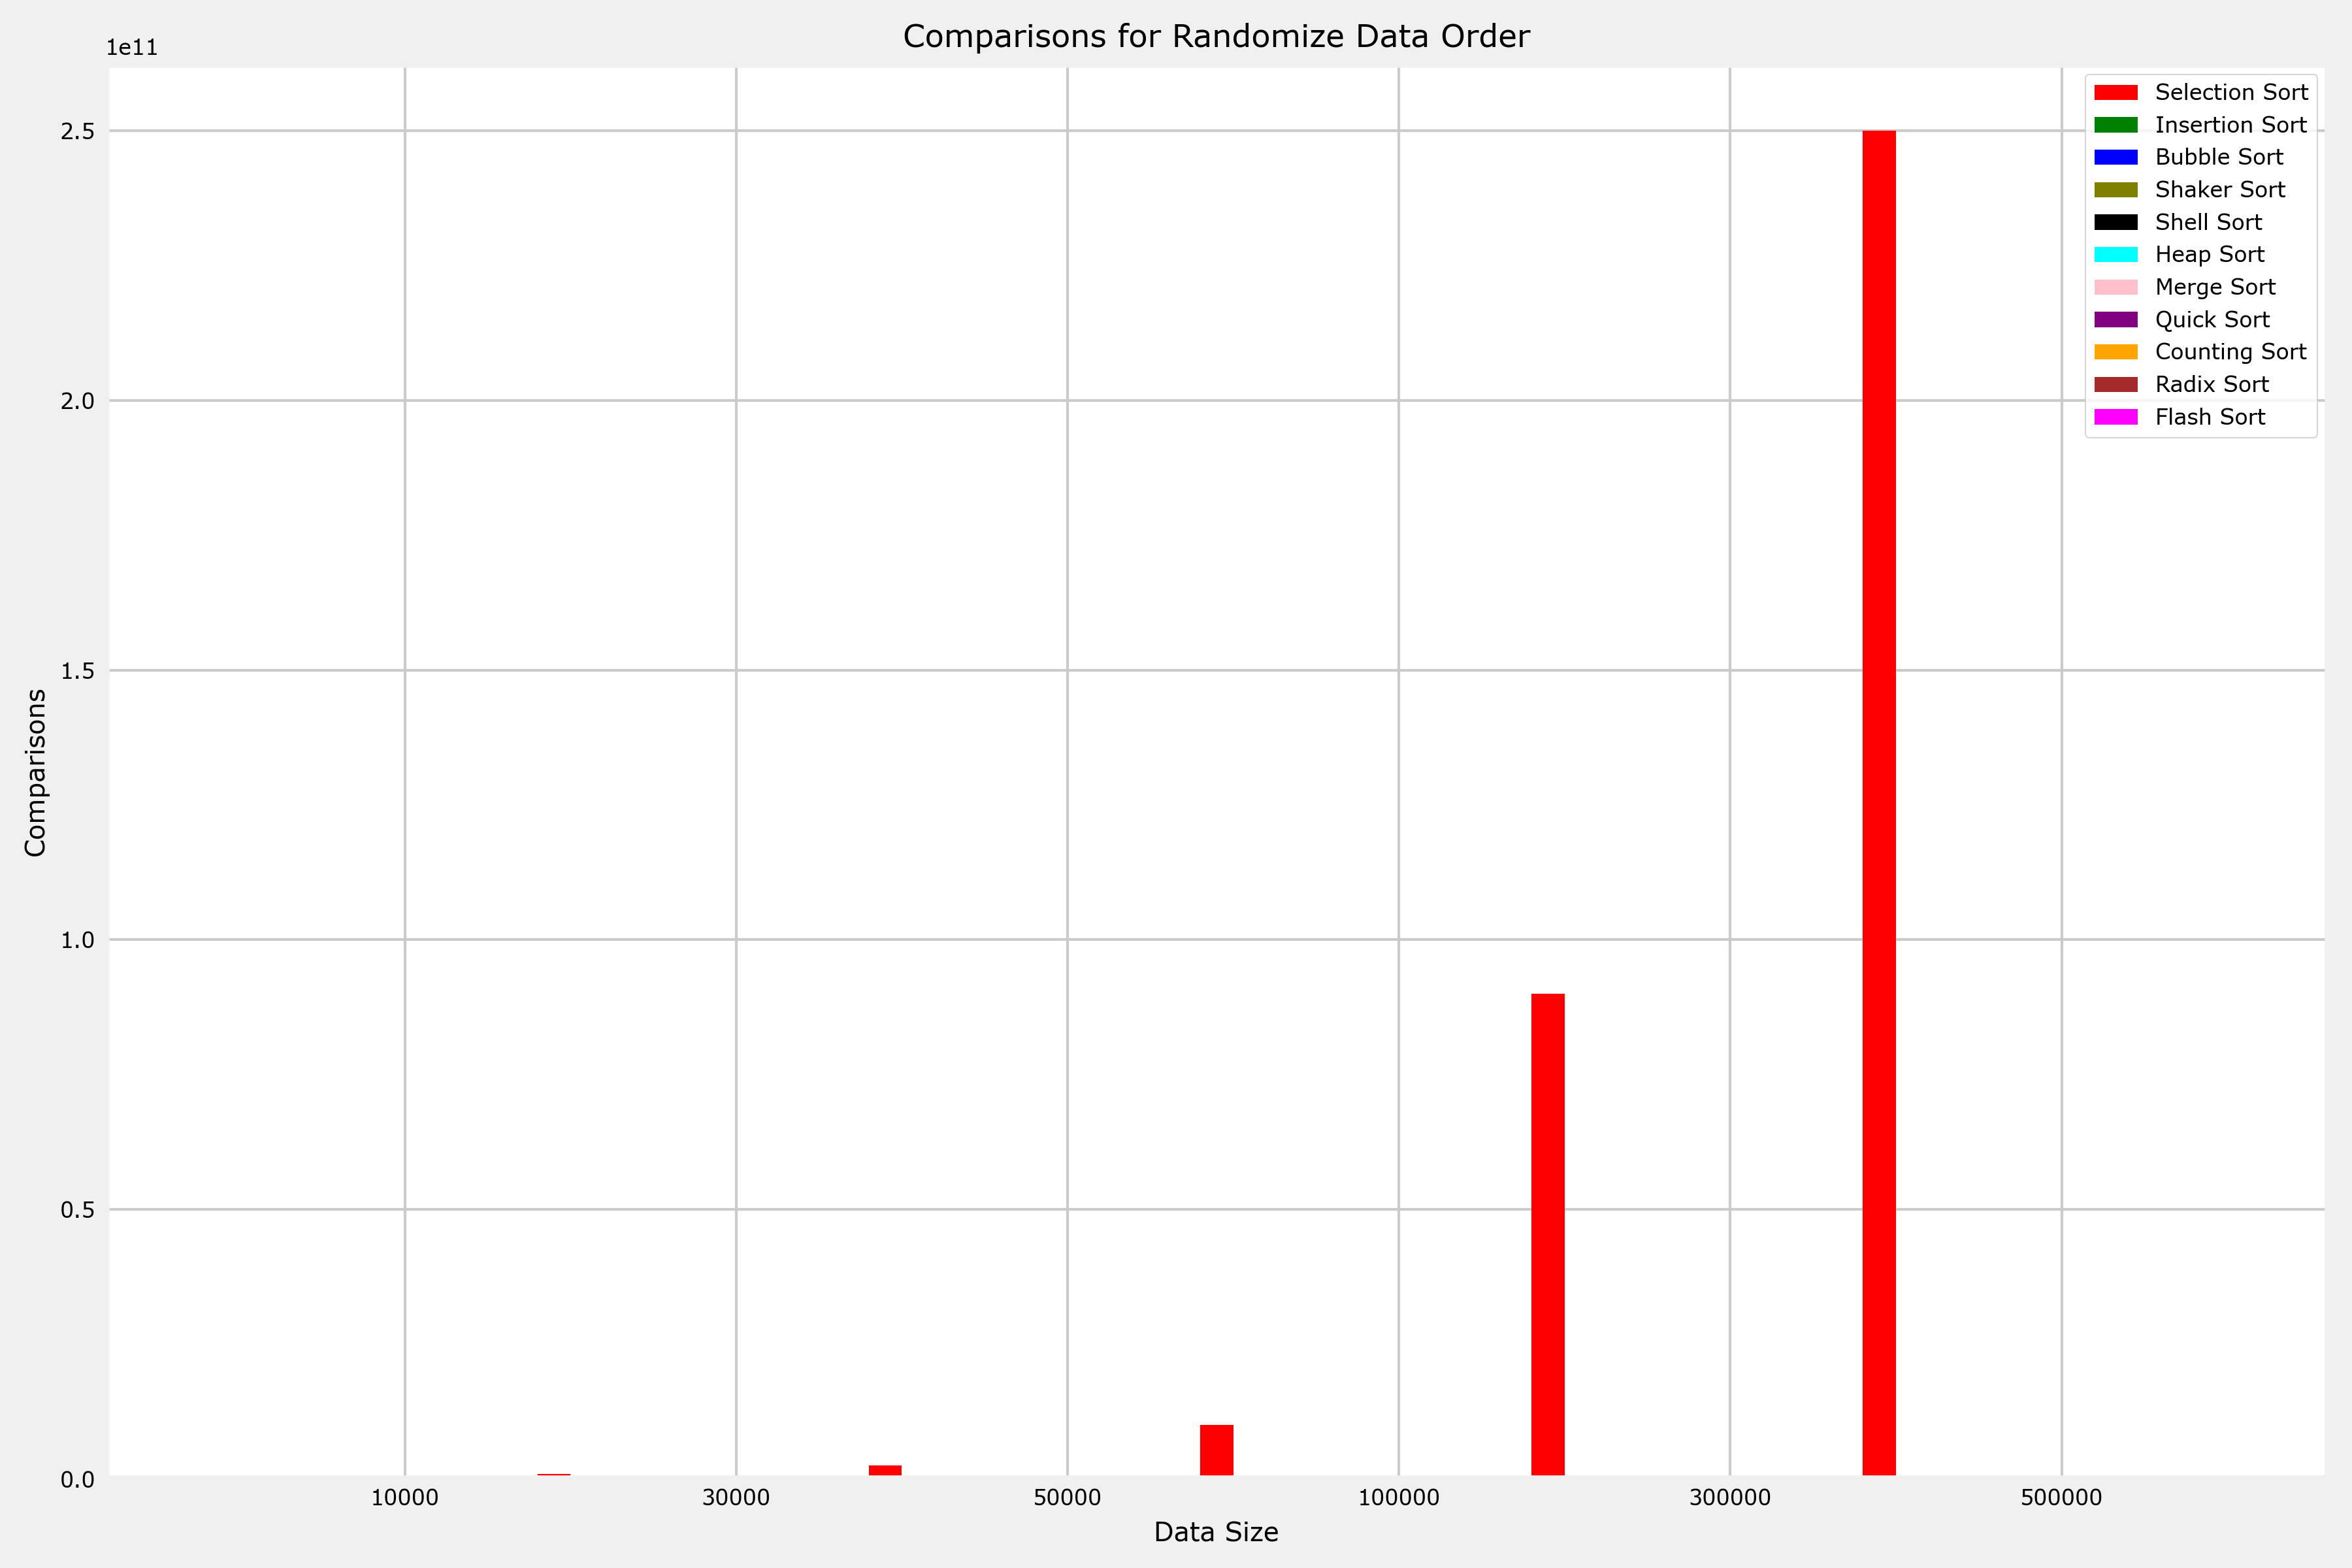
\includegraphics[width=0.8\textwidth]{img/results/randomize_comparisons.png}
    \caption{Số phép so sánh của 11 thuật toán với dữ liệu ngẫu nhiên}
\end{figure}

\begin{figure}[H]
    \centering
    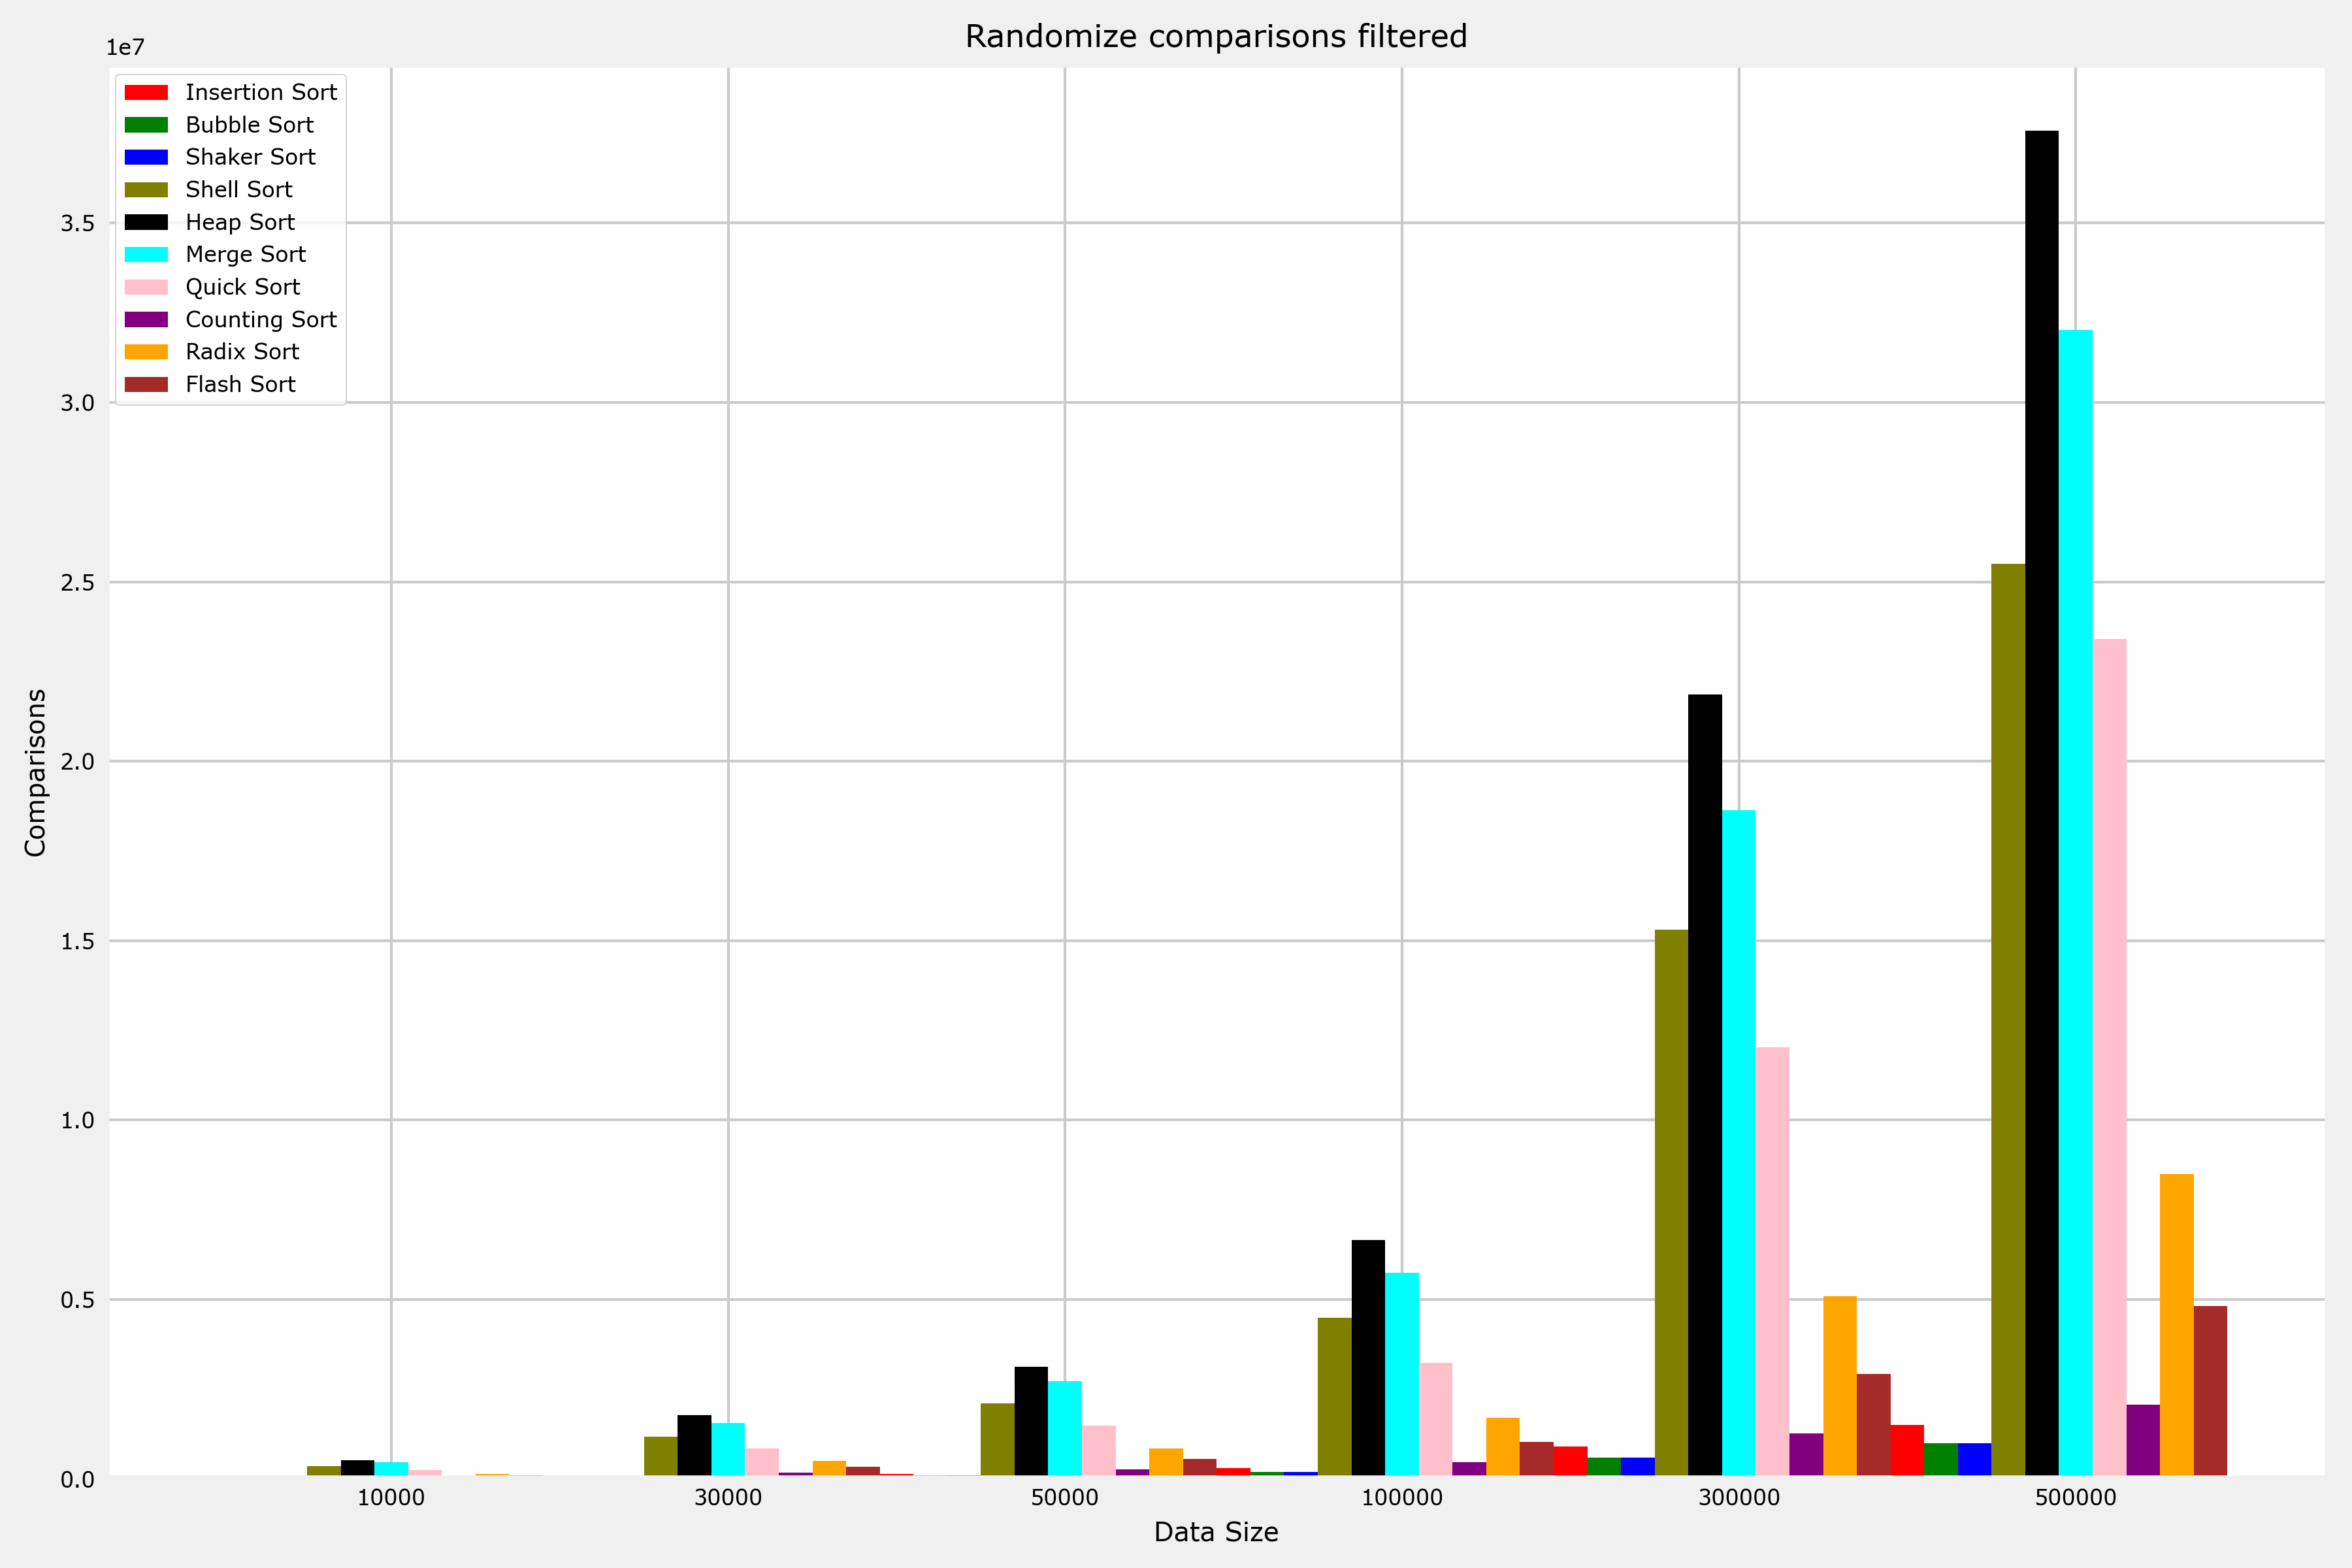
\includegraphics[width=0.8\textwidth]{img/results/randomize_comparisons_filtered.png}
    \caption{Số phép so sánh của 11 thuật toán với dữ liệu ngẫu nhiên sau khi loại bỏ outlier}
\end{figure}



\paragraph{2. Dữ liệu gần sắp xếp hoàn chỉnh}
\begin{figure}[H]
    \centering
    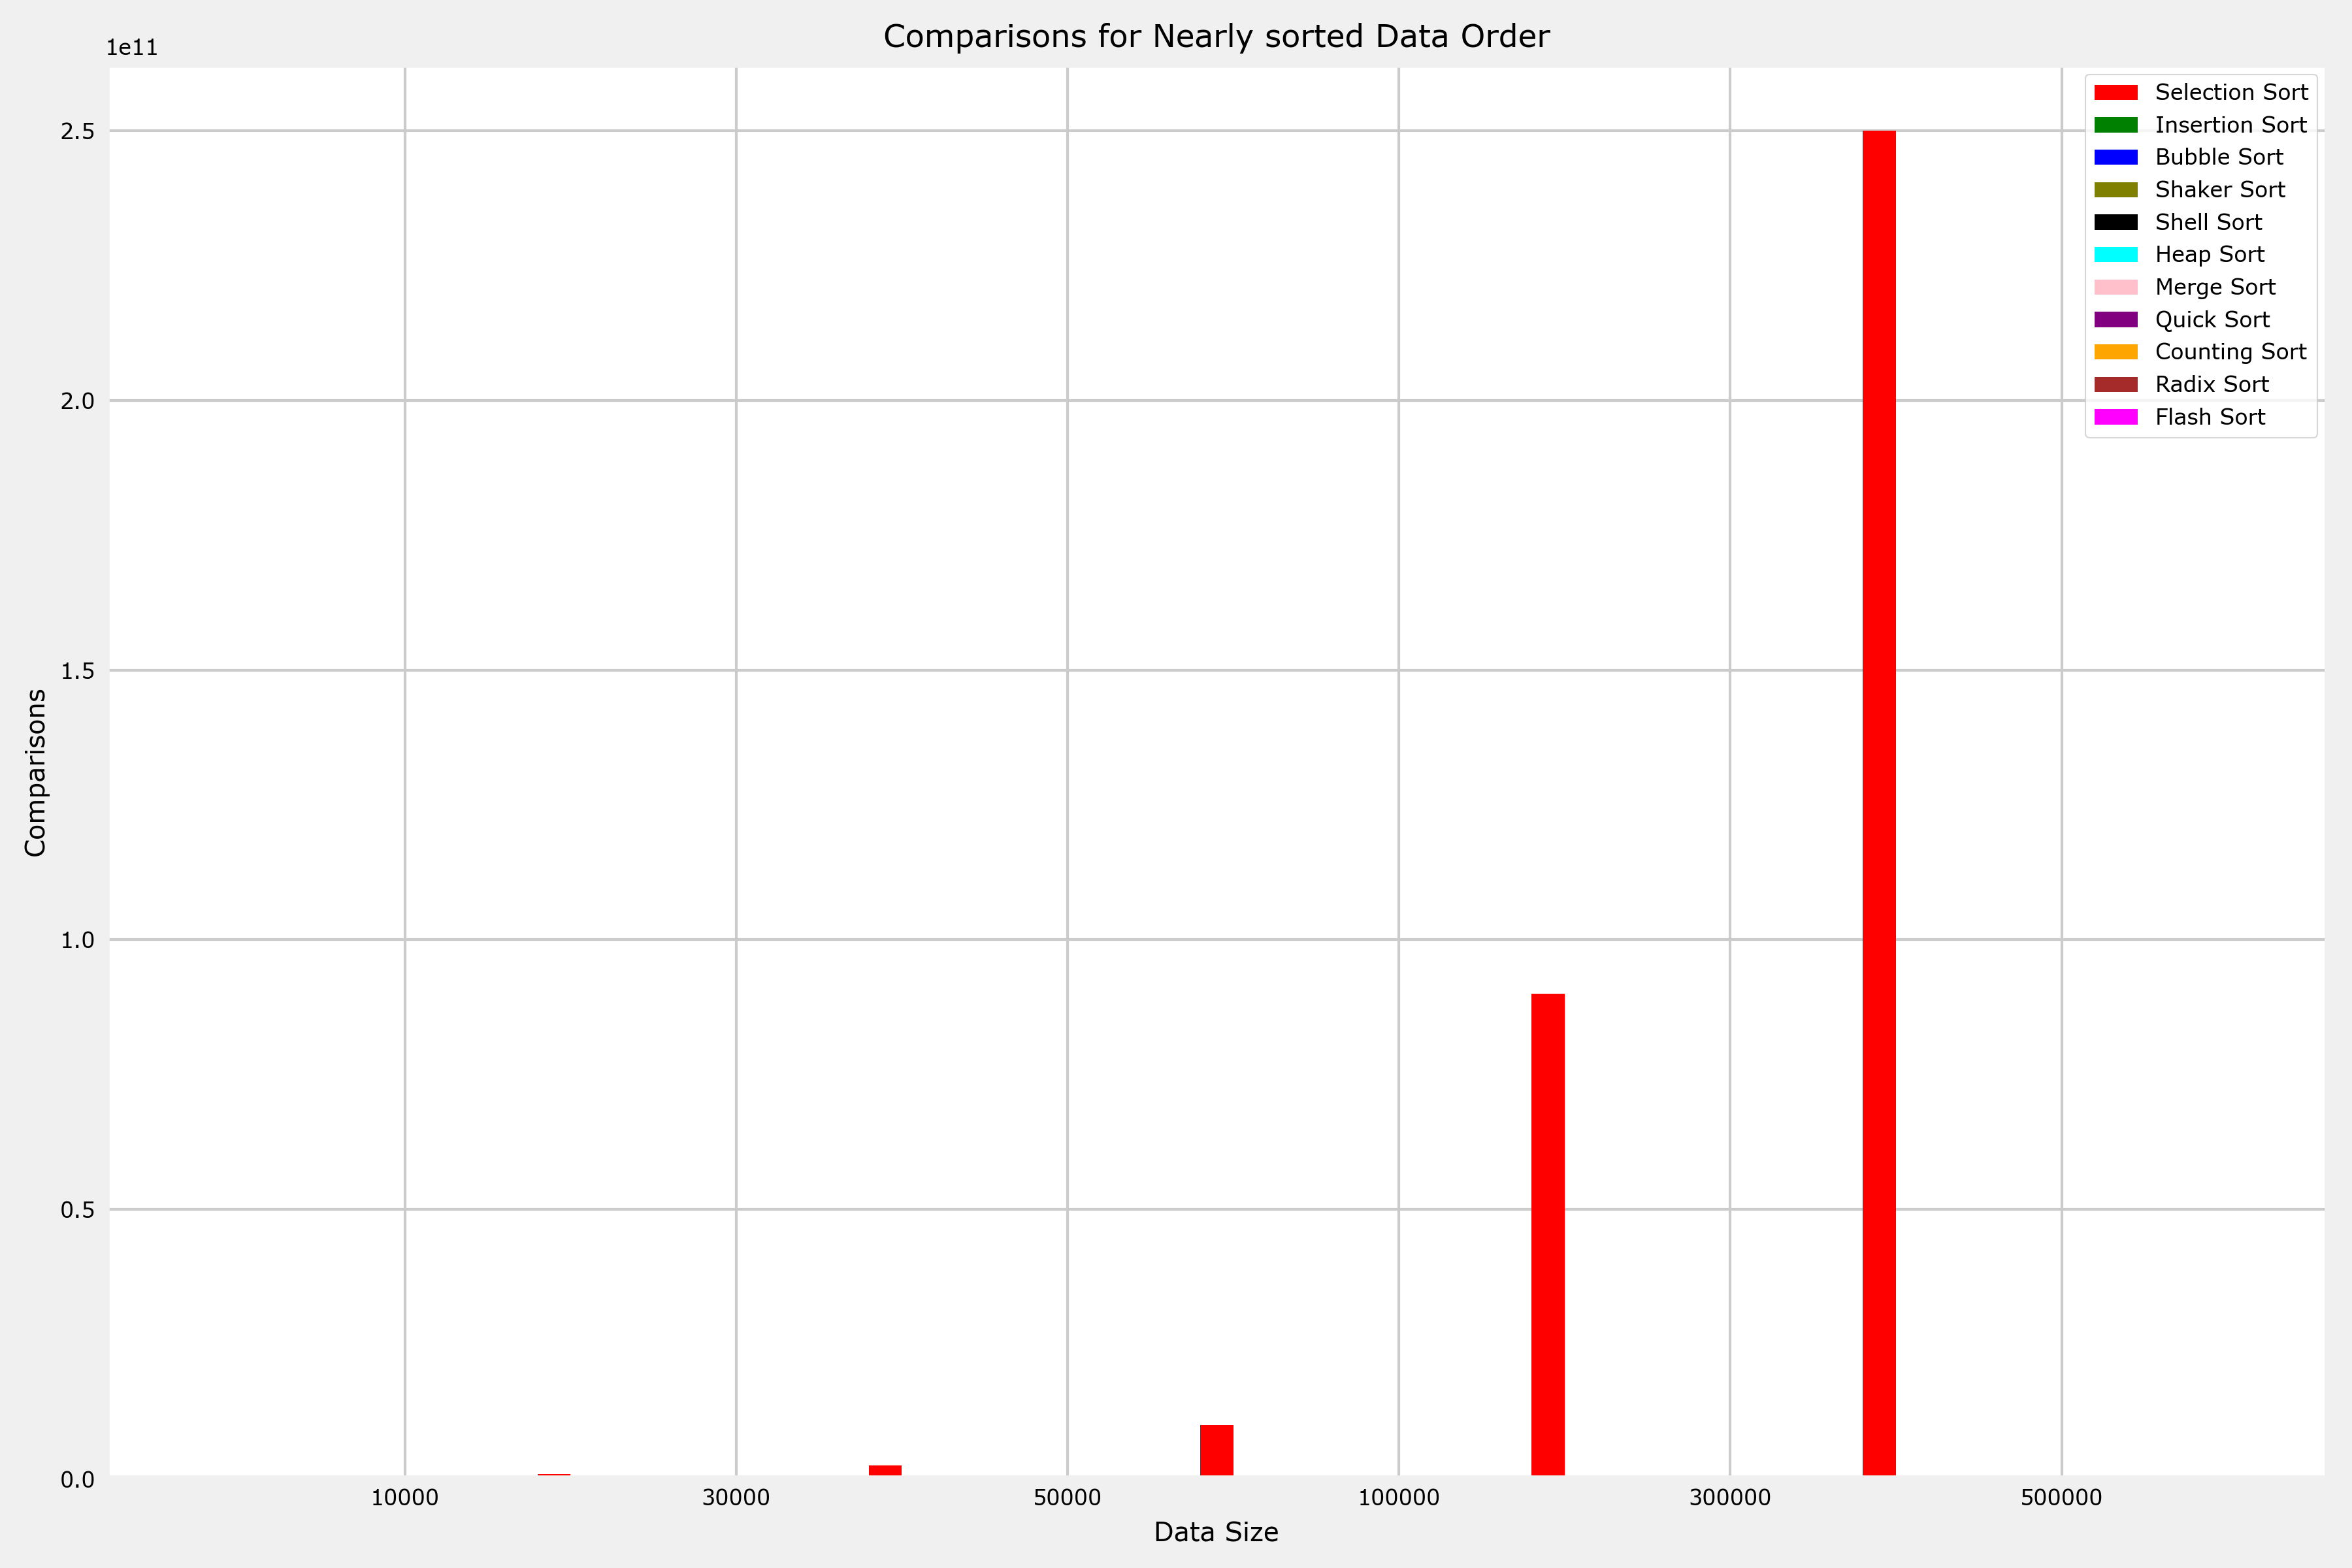
\includegraphics[width=0.8\textwidth]{img/results/nearly_sorted_comparisons.png}
    \caption{Số phép so sánh của 11 thuật toán với dữ liệu gần sắp xếp hoàn chỉnh}
\end{figure}

\begin{figure}[H]
    \centering
    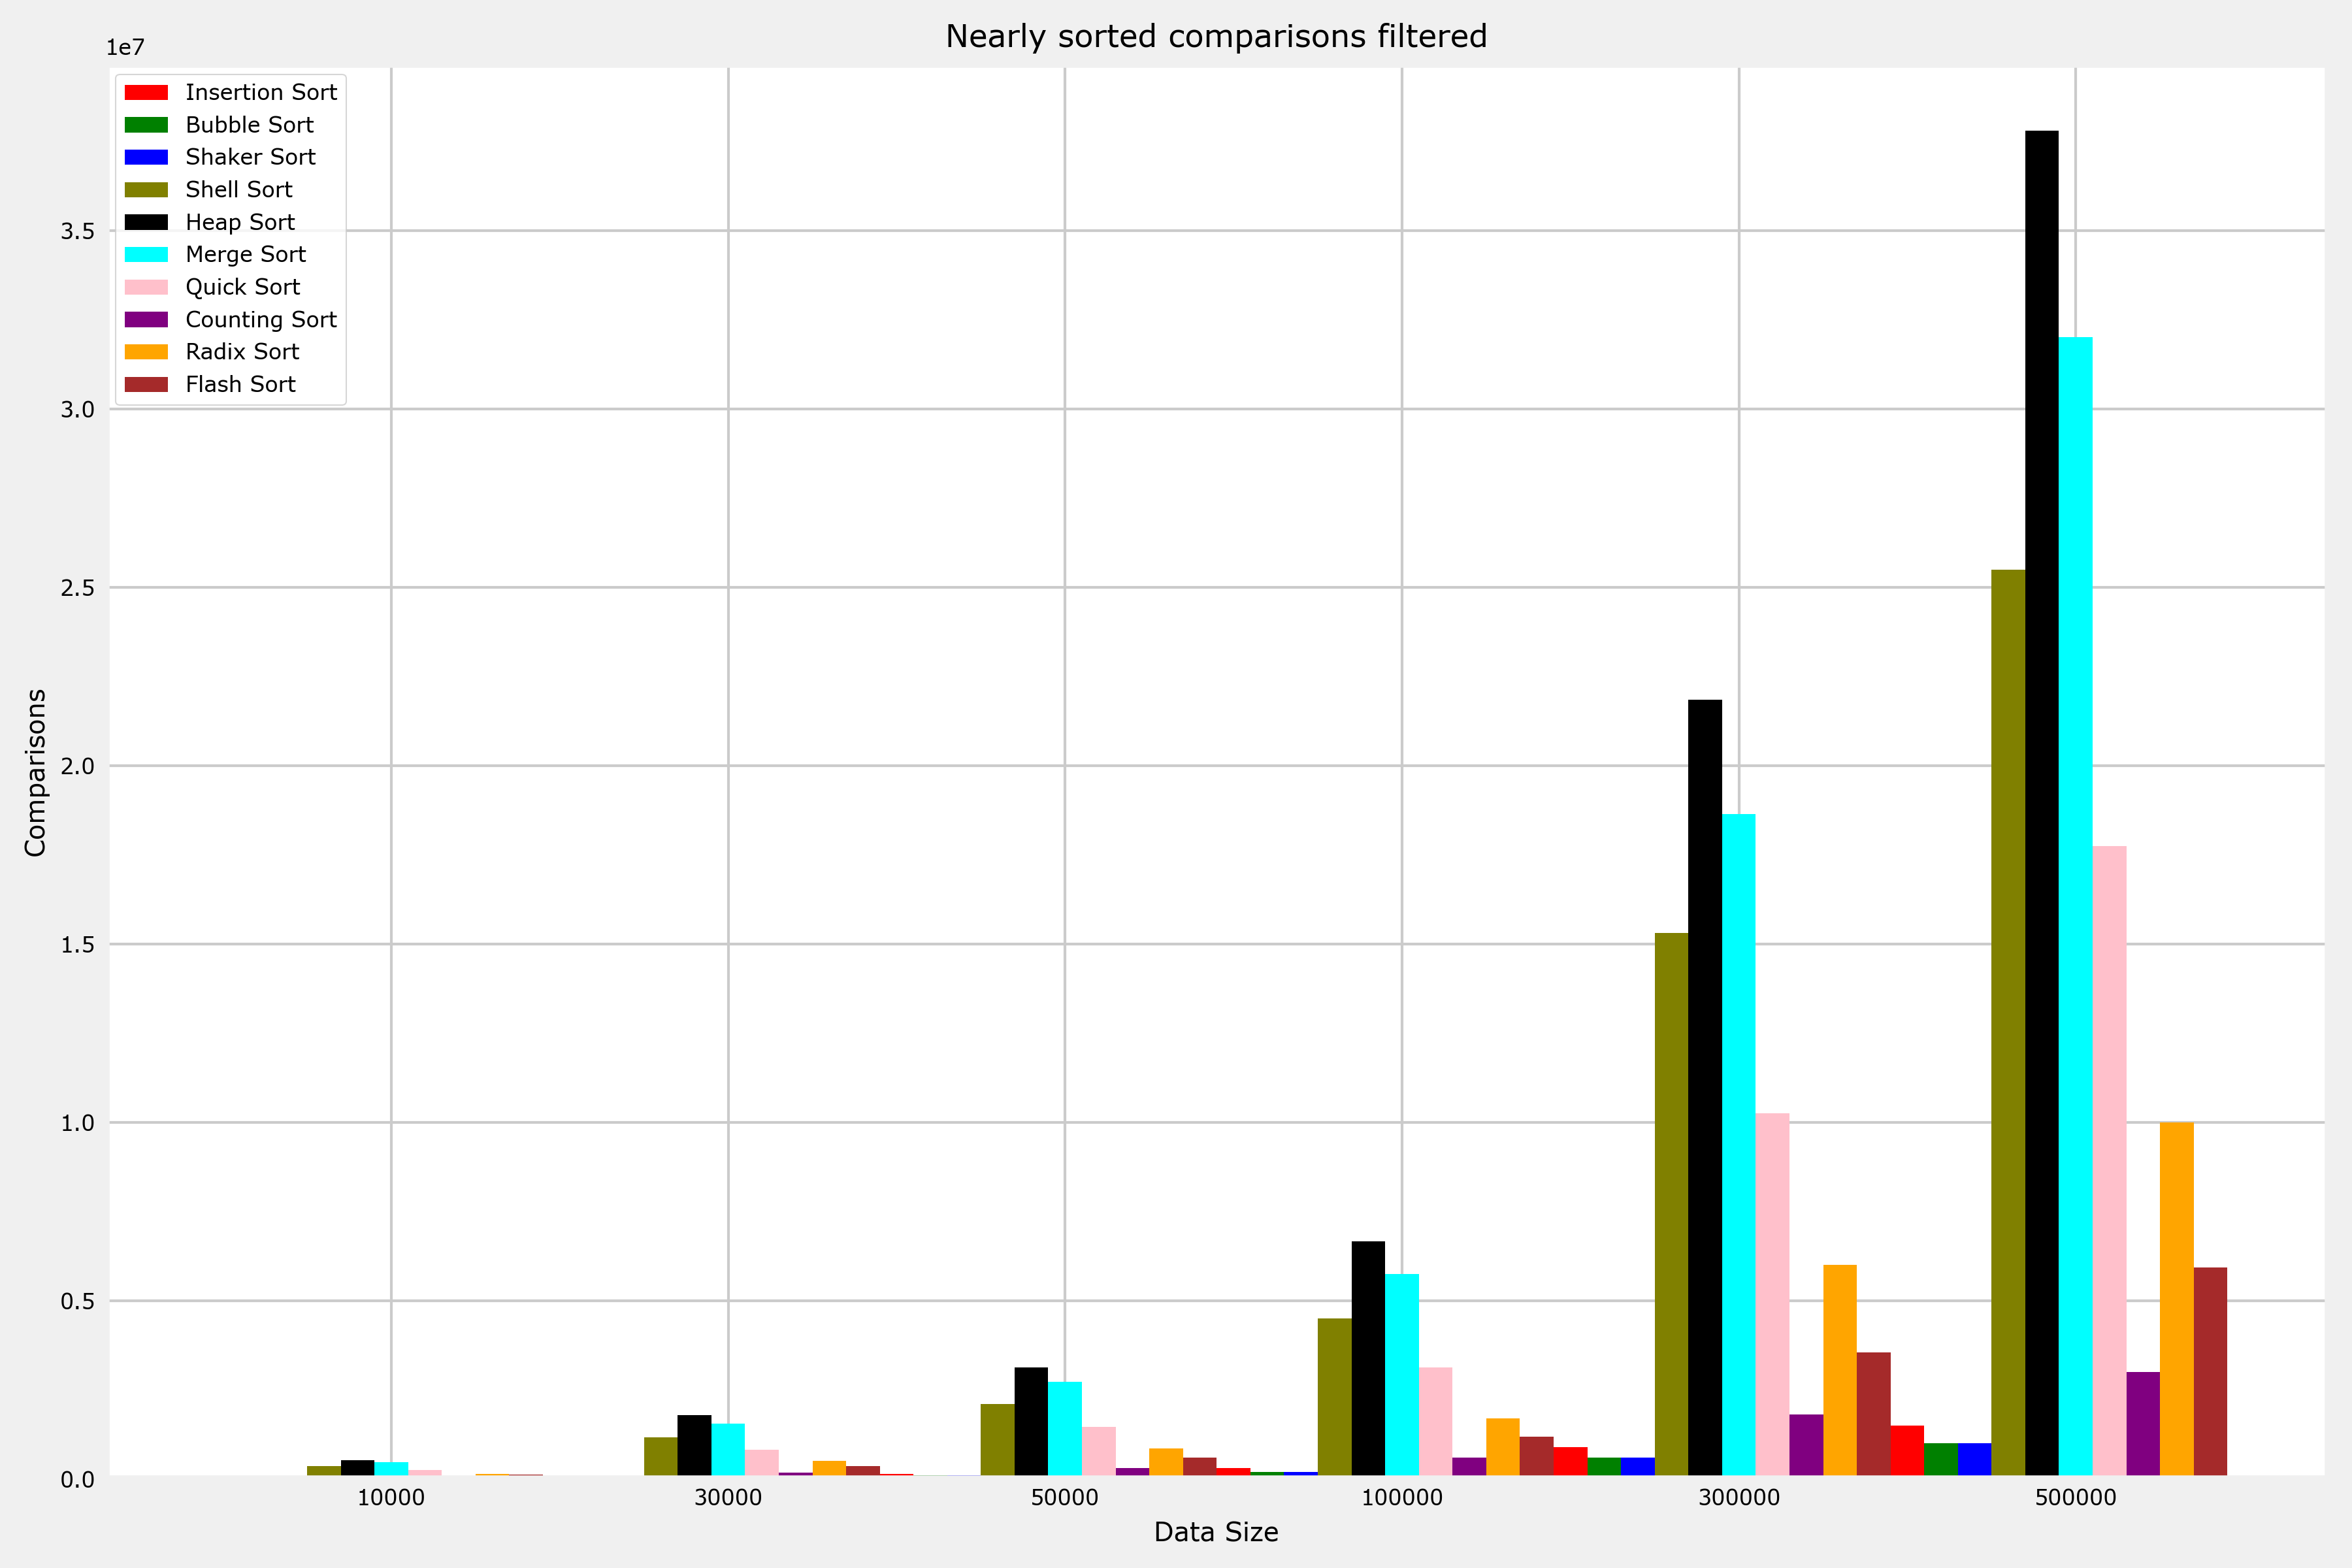
\includegraphics[width=0.8\textwidth]{img/results/nearly_sorted_comparisons_filtered.png}
    \caption{Số phép so sánh của 11 thuật toán với dữ liệu gần sắp xếp hoàn chỉnh sau khi loại bỏ outlier}
\end{figure}


\paragraph{3. Dữ liệu được sắp xếp}
\begin{figure}[H]
    \centering
    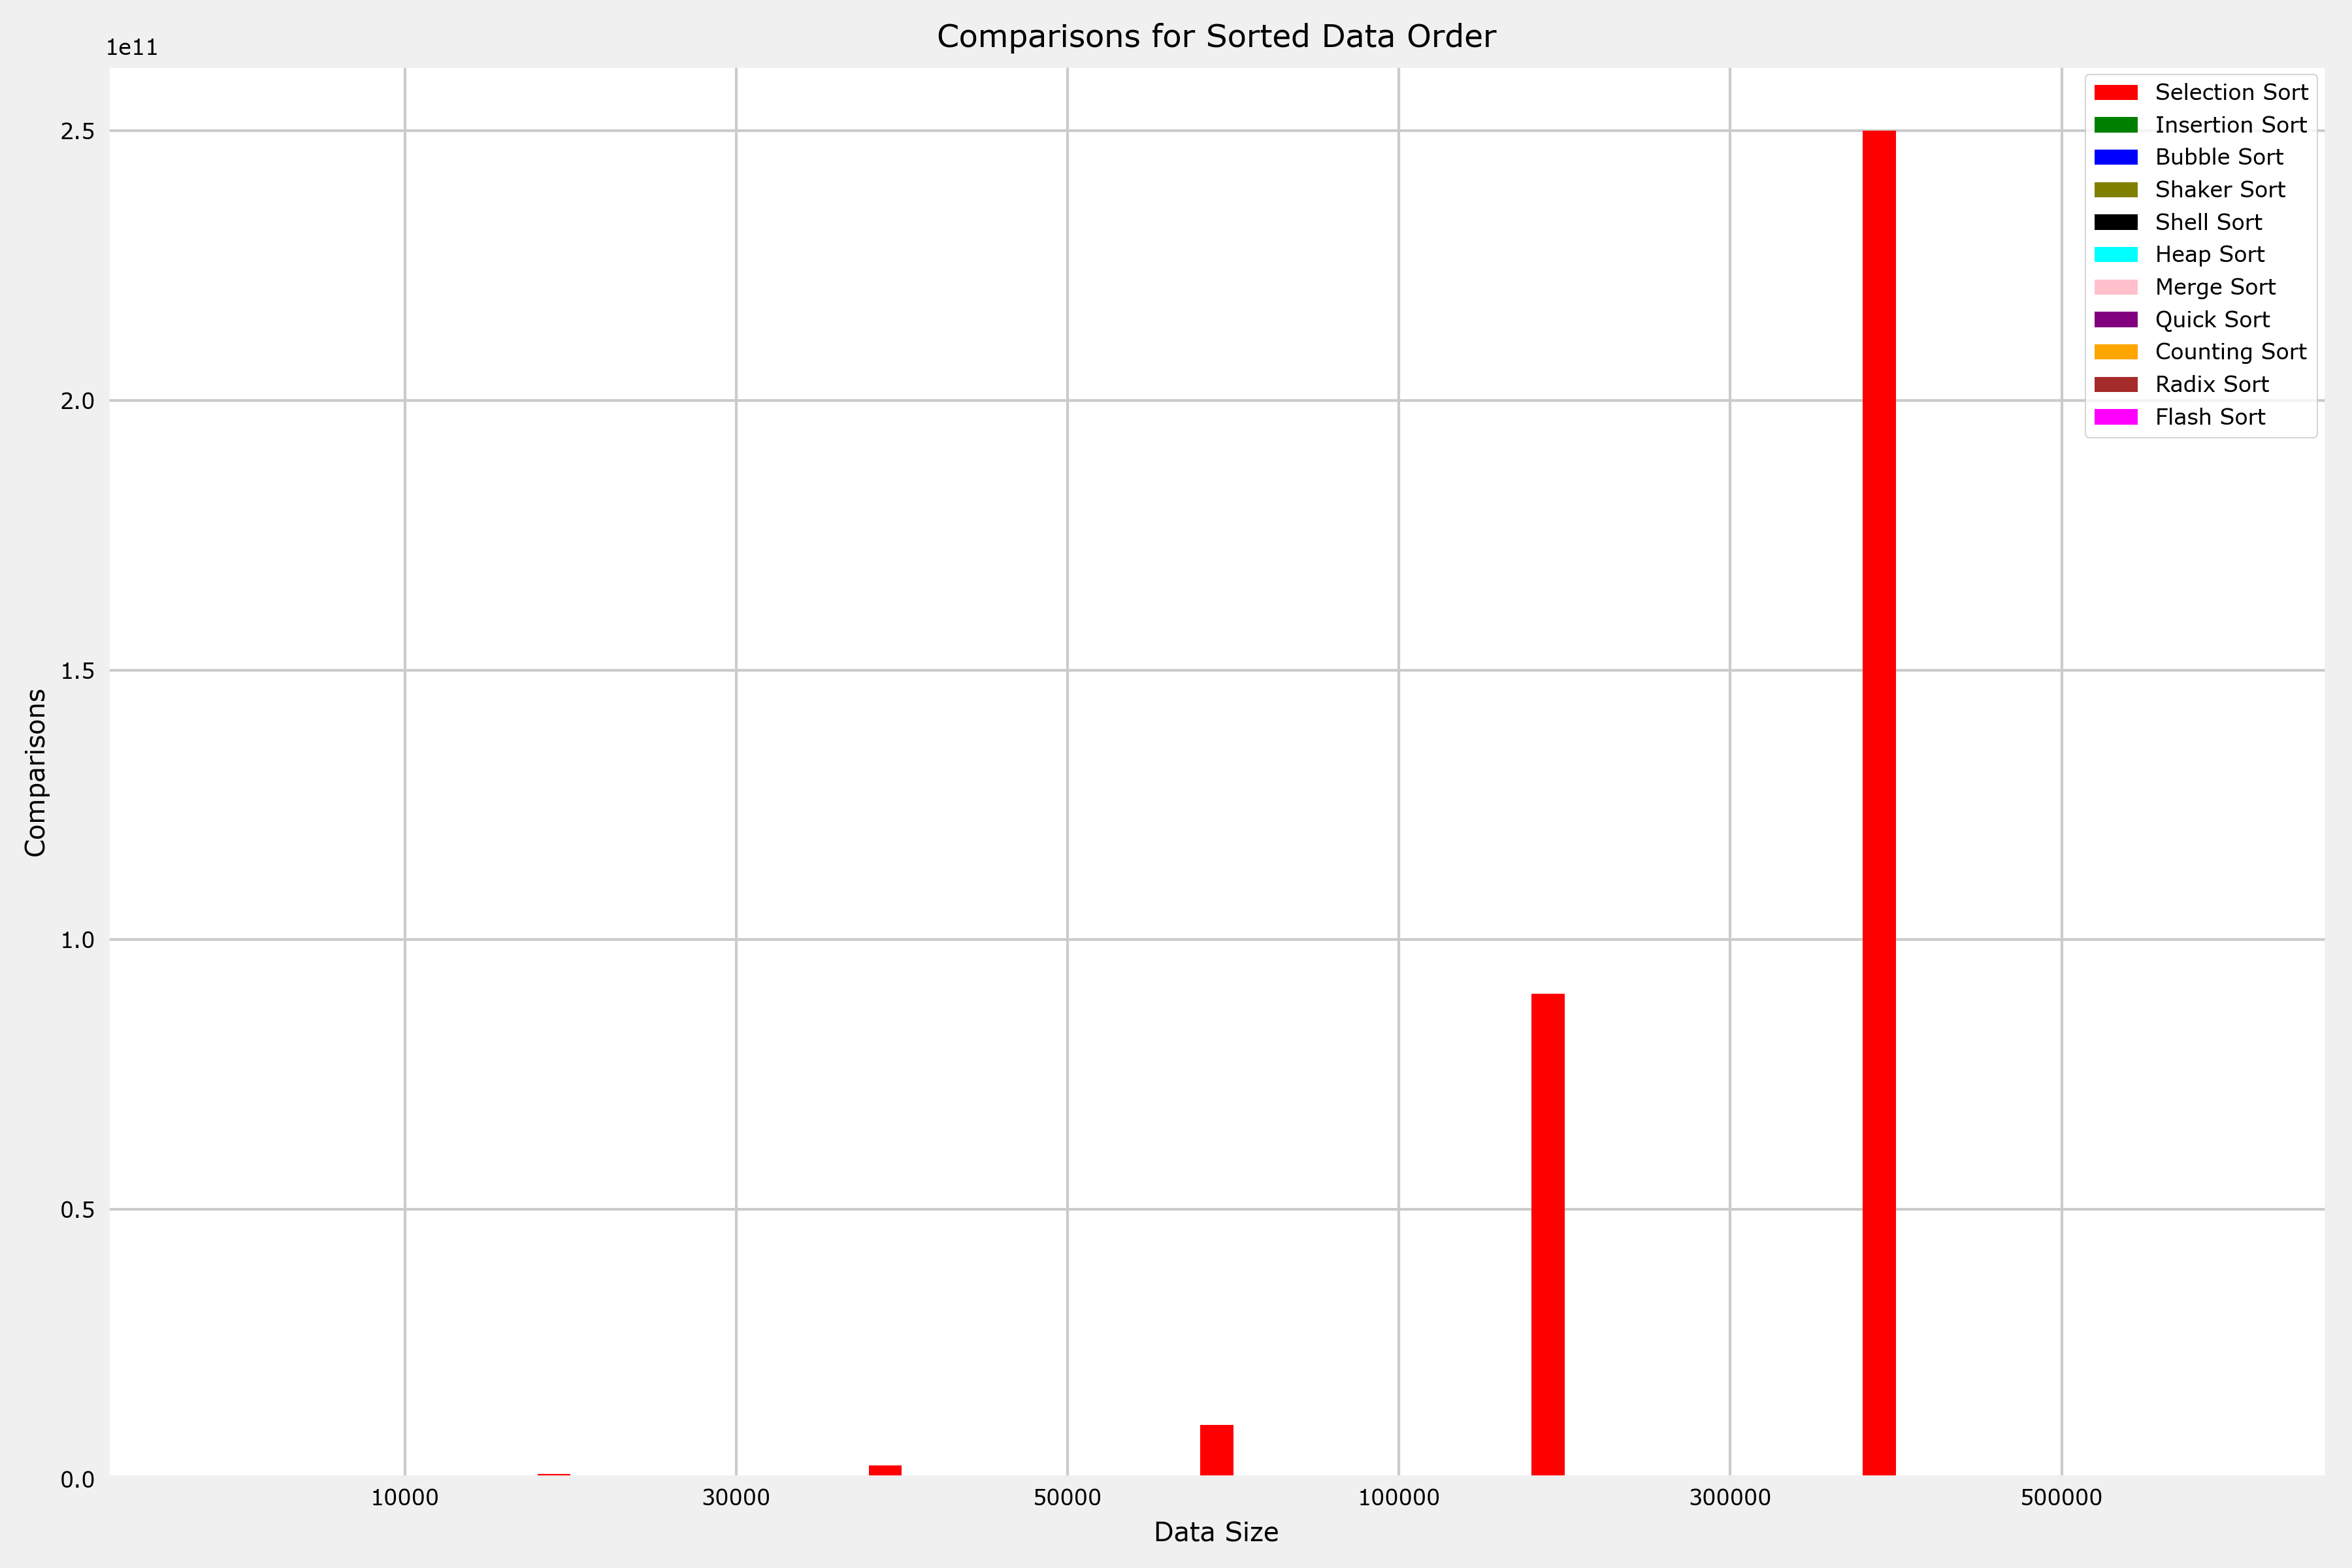
\includegraphics[width=0.8\textwidth]{img/results/sorted_comparisons.png}
    \caption{Số phép so sánh của 11 thuật toán với dữ liệu được sắp xếp}
\end{figure}

\begin{figure}[H]
    \centering
    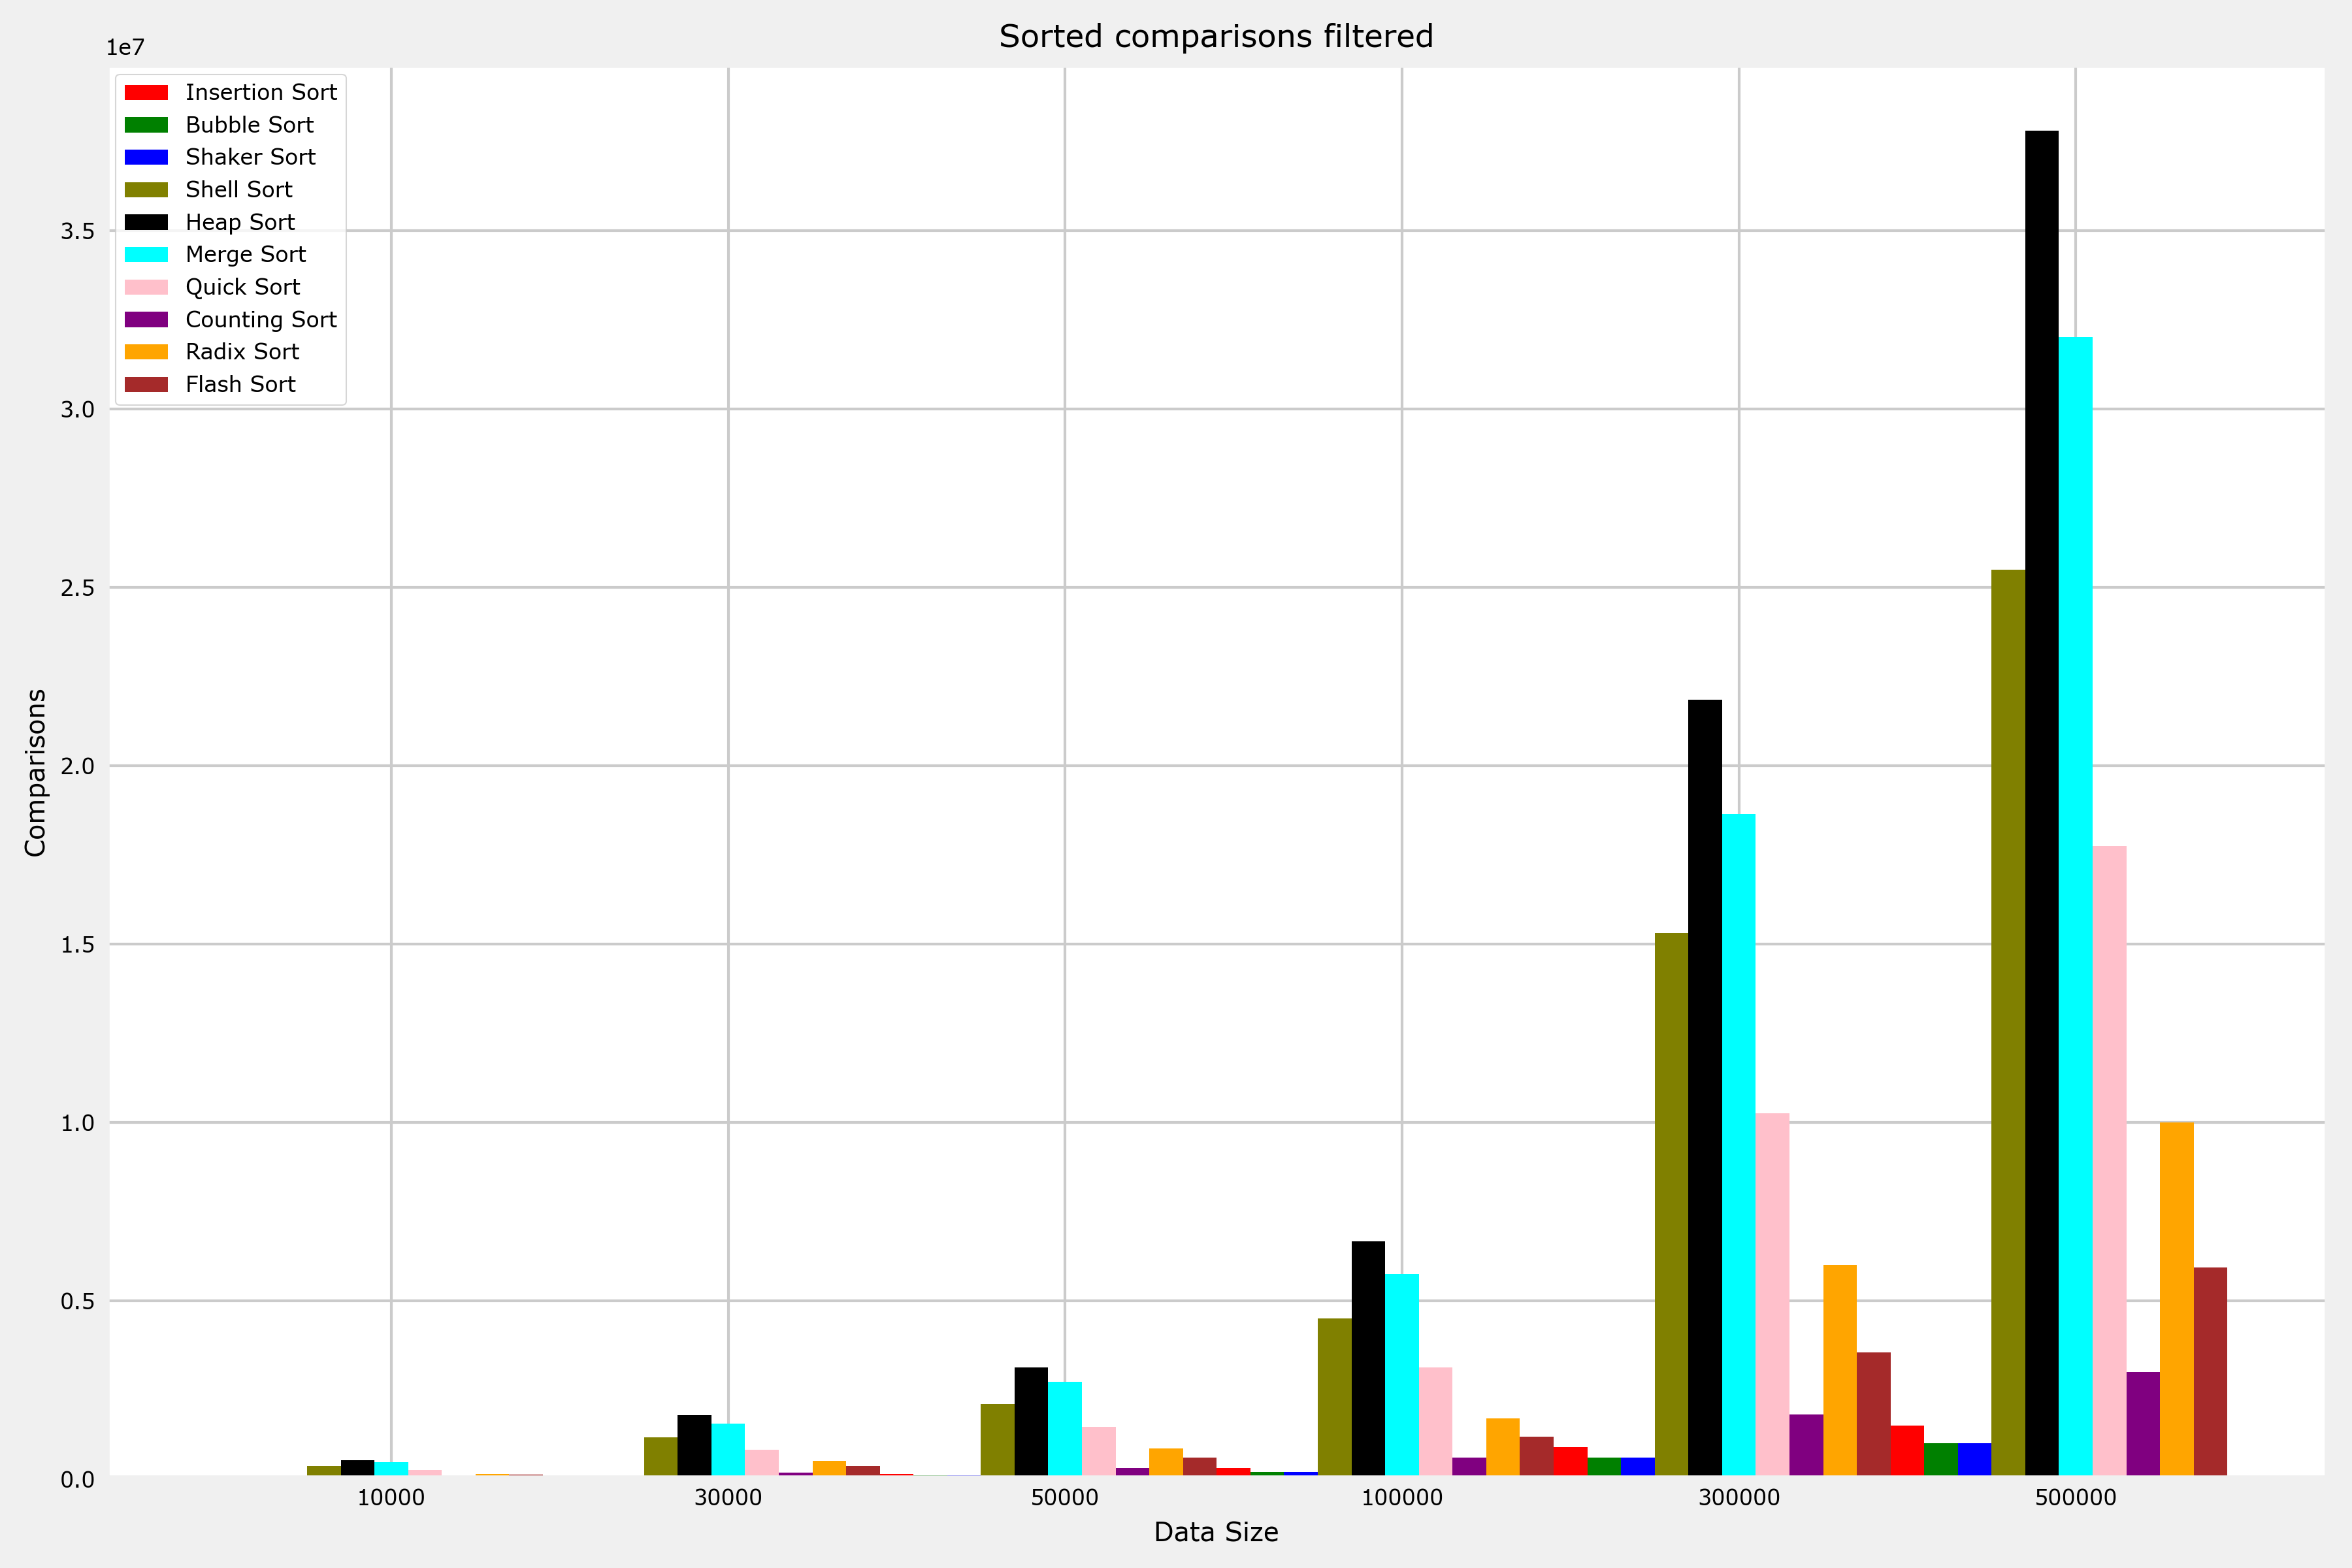
\includegraphics[width=0.8\textwidth]{img/results/sorted_comparisons_filtered.png}
    \caption{Số phép so sánh của 11 thuật toán với dữ liệu được sắp xếp sau khi loại bỏ outlier}
\end{figure}




\paragraph{4. Dữ liệu đảo ngược}
\begin{figure}[H]
    \centering
    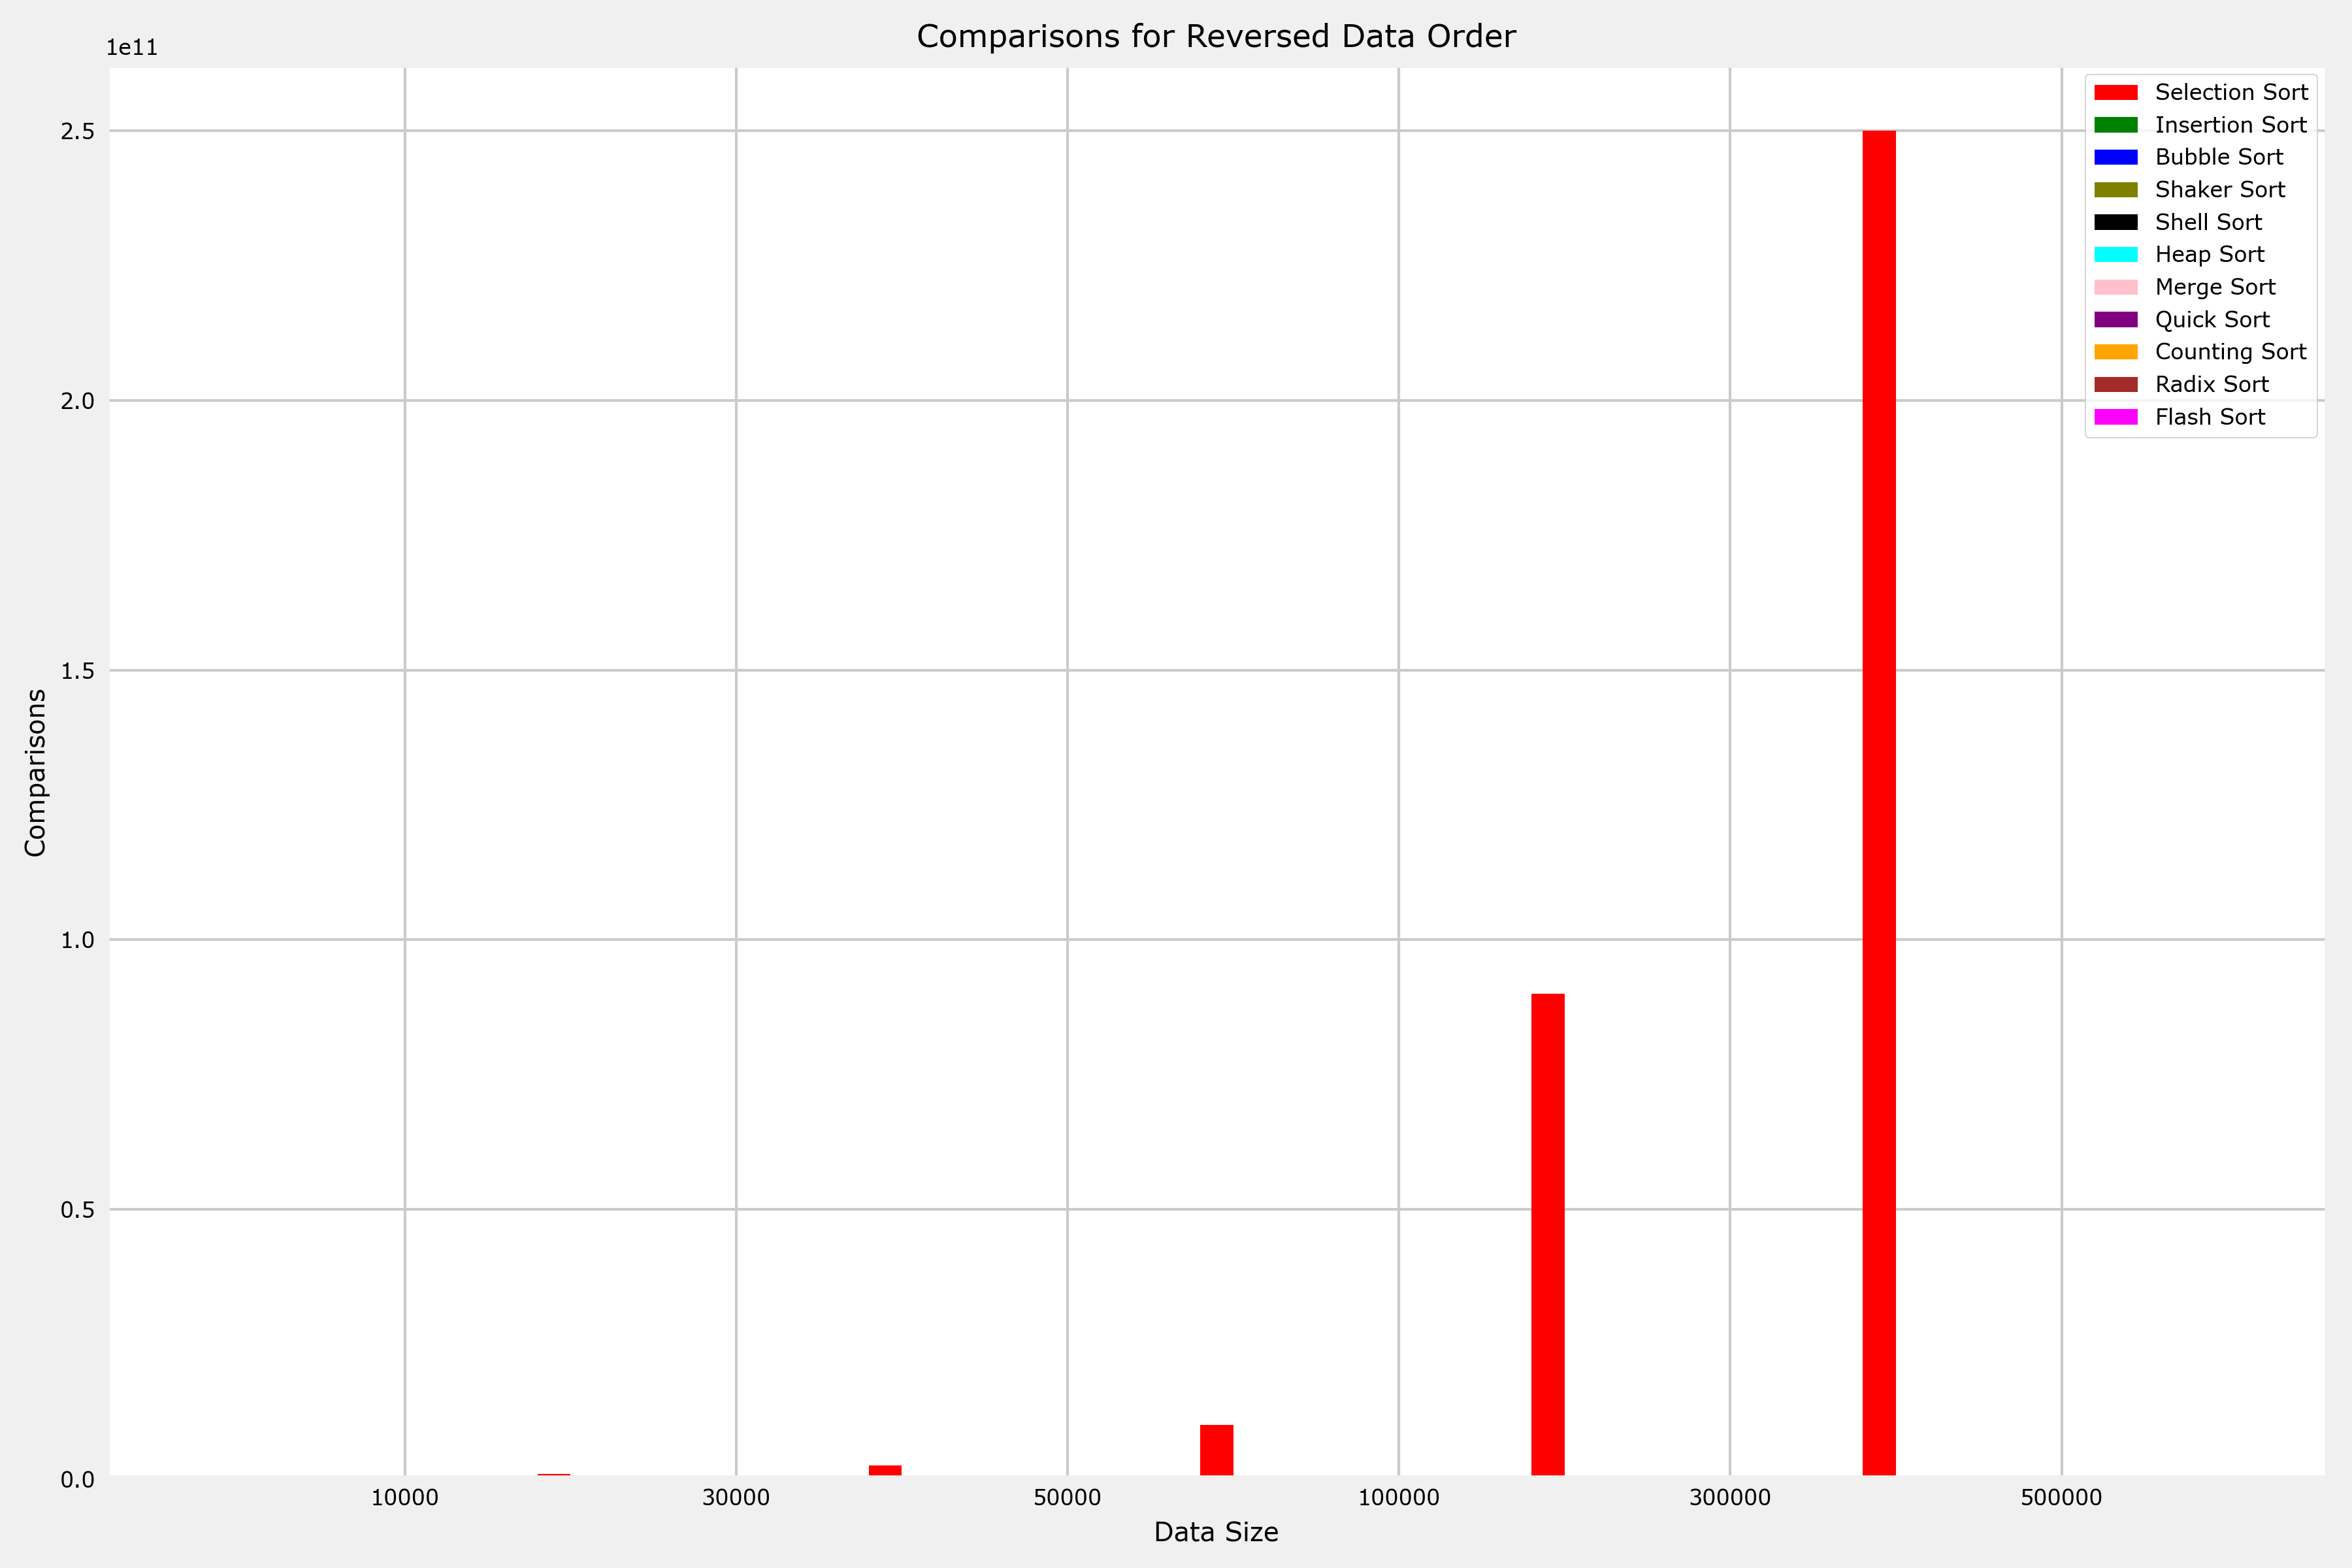
\includegraphics[width=0.8\textwidth]{img/results/reversed_comparisons.png}
    \caption{Số phép so sánh của 11 thuật toán với dữ liệu đảo ngược}
\end{figure}

\begin{figure}[H]
    \centering
    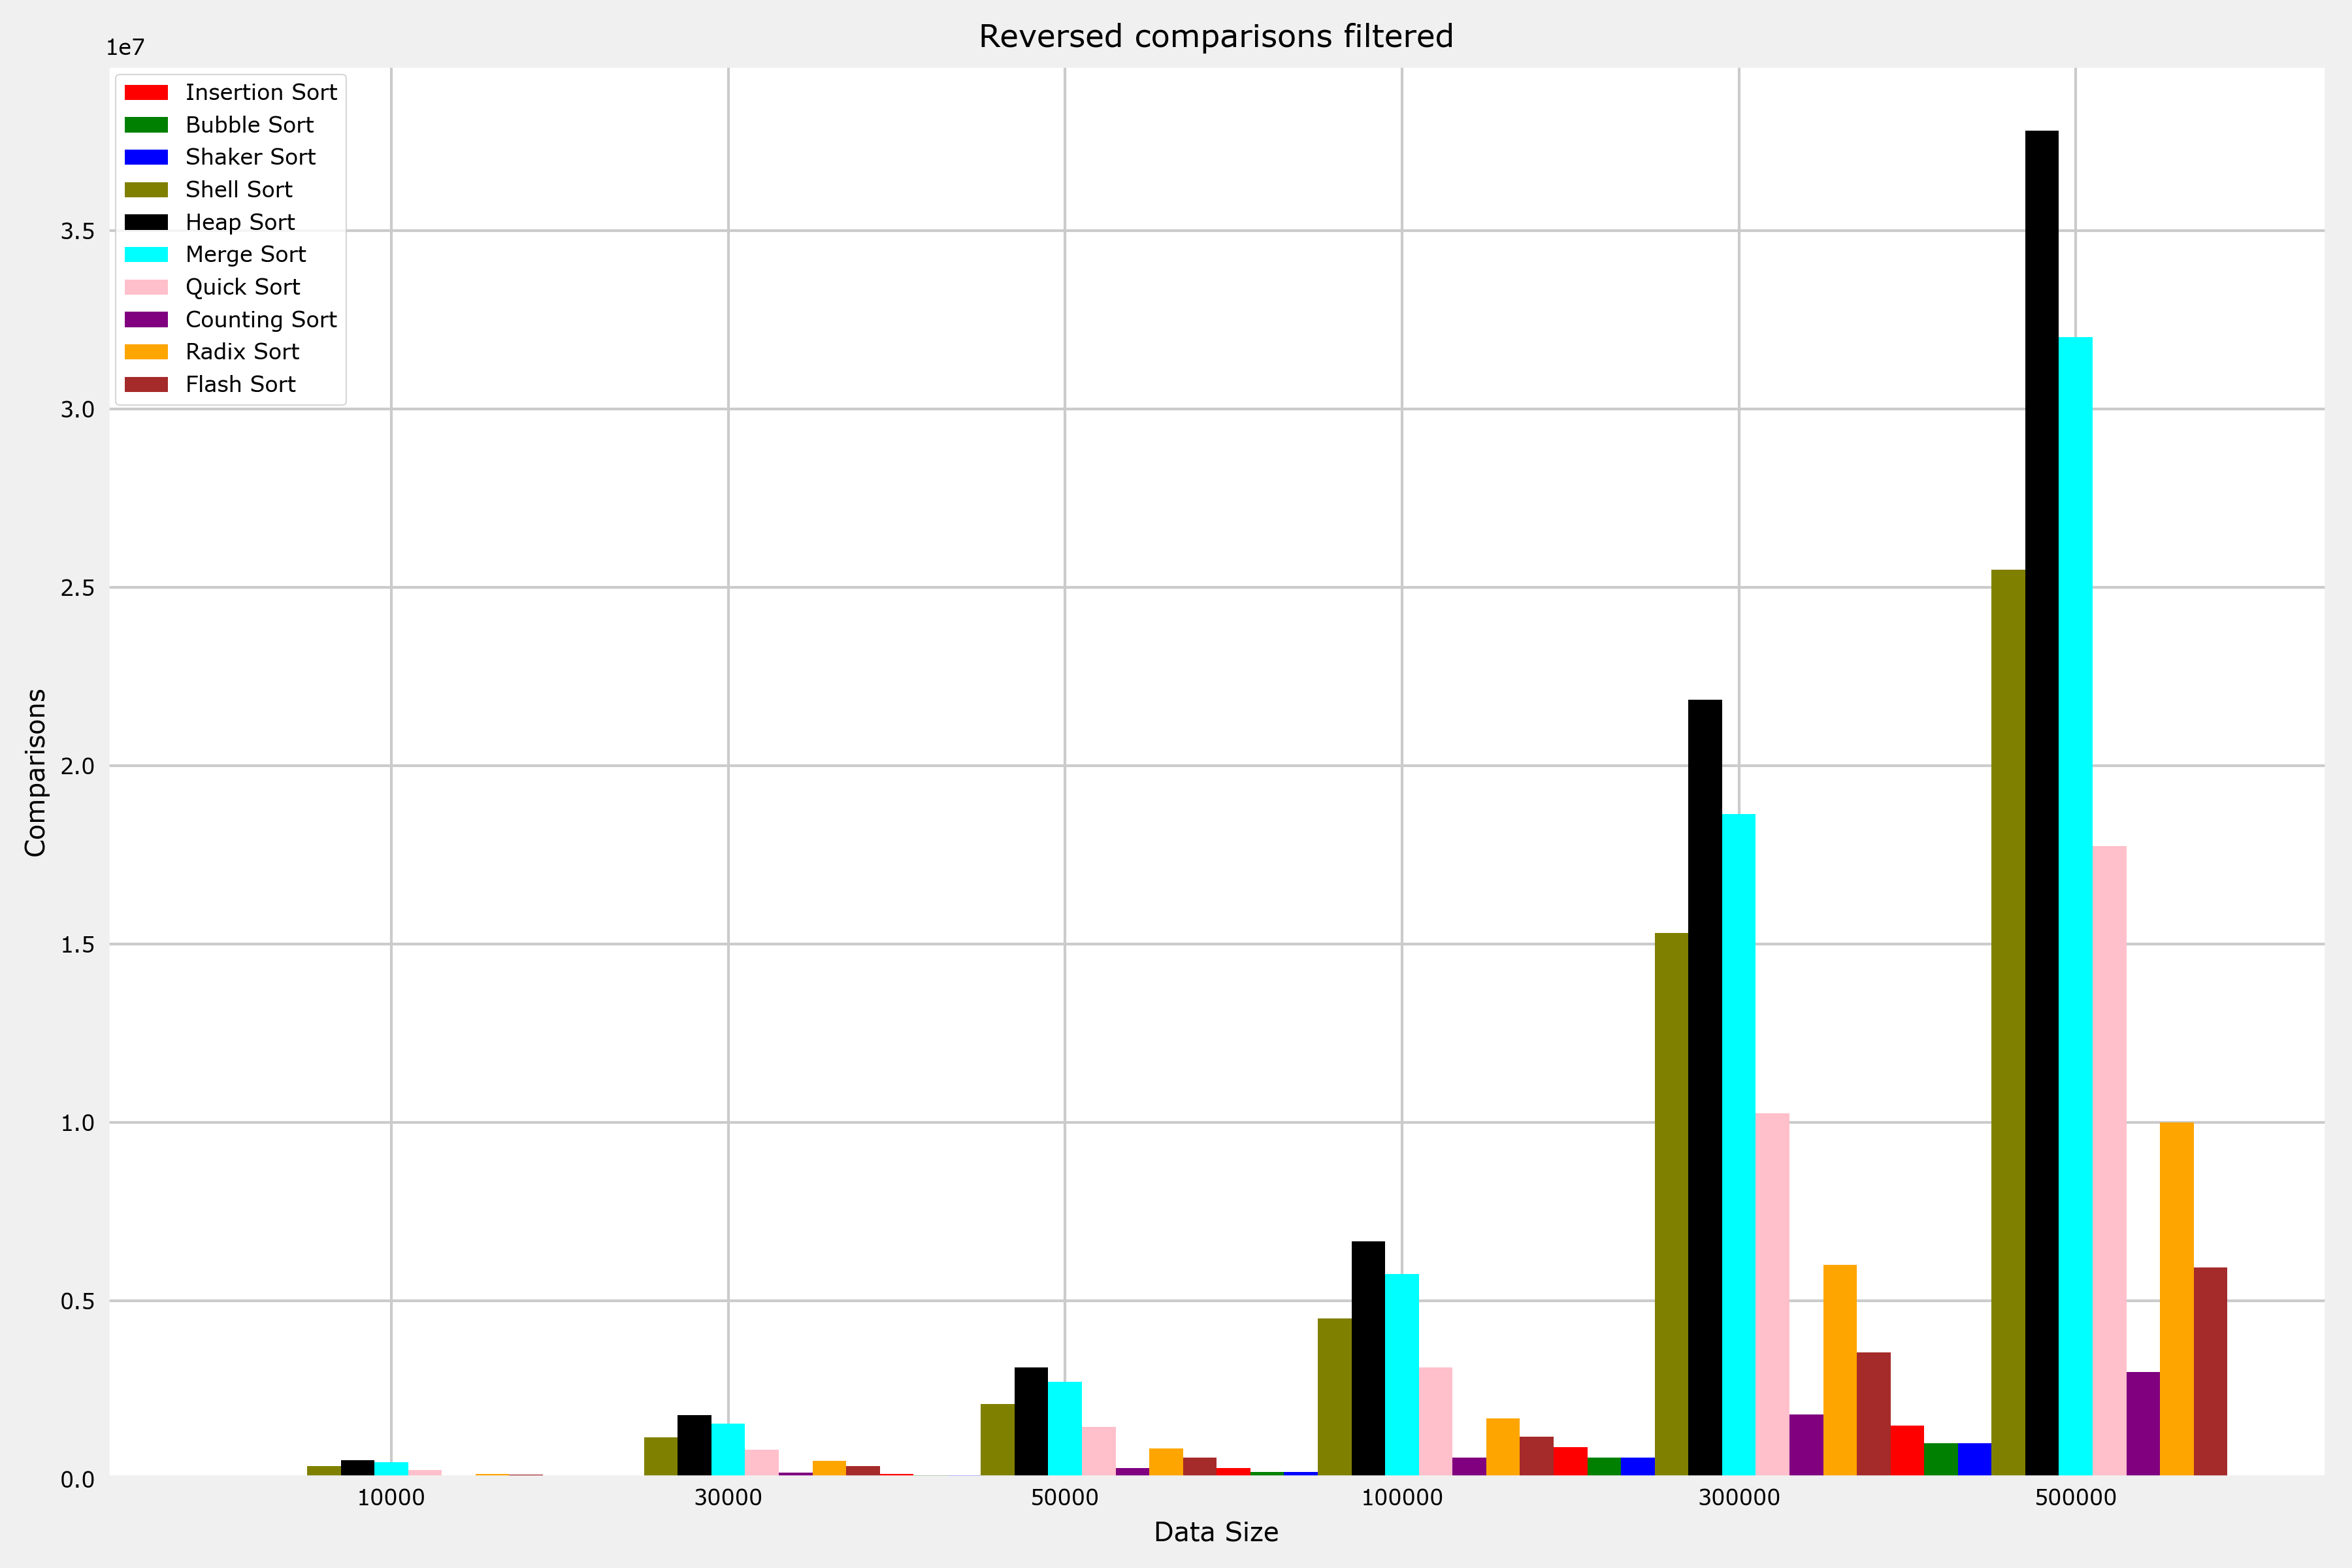
\includegraphics[width=0.8\textwidth]{img/results/reversed_comparisons_filtered.png}
    \caption{
        Số phép so sánh của 11 thuật toán với dữ liệu đảo ngược sau khi loại bỏ outlier
    }
\end{figure}

\textbf{Nhận xét chung}

Các biểu đồ và hình ảnh trong phần kết quả thực nghiệm cho thấy sự khác biệt rõ rệt về hiệu suất của các thuật toán sắp xếp khi áp dụng trên các bộ dữ liệu khác nhau. 

1. **Dữ liệu ngẫu nhiên**: Các thuật toán cơ bản như Bubble Sort và Shaker Sort có thời gian chạy lớn hơn rất nhiều so với các thuật toán khác, thể hiện rõ độ phức tạp $O(n^2)$. Trong khi đó, các thuật toán như Counting Sort và Flash Sort có thời gian chạy rất nhỏ và ổn định.

2. **Dữ liệu gần sắp xếp hoàn chỉnh**: Insertion Sort có thời gian thực thi nhanh nhất, phù hợp với trường hợp tốt nhất của nó. Các thuật toán cải tiến và không so sánh như Heap Sort, Radix Sort, Merge Sort vẫn giữ được tính ổn định.

3. **Dữ liệu được sắp xếp**: Shaker Sort và Insertion Sort là hai thuật toán nhanh nhất, phù hợp với độ phức tạp thời gian $\Theta(n)$ trong trường hợp tốt nhất. Các thuật toán khác như Heap Sort, Radix Sort, Merge Sort vẫn giữ được tính ổn định.

4. **Dữ liệu đảo ngược**: Shaker Sort có thời gian chạy chậm hơn Bubble Sort, trong khi Selection Sort và Insertion Sort có thời gian thực thi tương đối giống nhau. Các thuật toán như Heap Sort, Radix Sort, Merge Sort vẫn thể hiện được tính ổn định.

5. **Số phép so sánh**: Selection Sort có số lượng phép so sánh vượt trội, đạt đến 2500049999 phép so sánh. Các thuật toán khác được chia thành ba nhóm chính: Nhóm 1 (Insertion Sort, Bubble Sort, Shaker Sort) có số lượng phép so sánh ít nhất, Nhóm 2 (Shell Sort, Heap Sort, Merge Sort, Quick Sort) có số phép so sánh nhiều nhất, và Nhóm 3 (Counting Sort, Radix Sort, Flash Sort) có số phép so sánh ổn định và thấp nhất.

Nhìn chung, các thuật toán cải tiến và không so sánh như Counting Sort, Flash Sort, Heap Sort, Radix Sort, Merge Sort thể hiện hiệu suất tốt và ổn định hơn so với các thuật toán cơ bản như Bubble Sort, Shaker Sort, và Selection Sort.